\documentclass[encoding=utf8,british]{template/thesis}
\usepackage[OT1]{fontenc}

\usepackage{algorithm}
\usepackage{algpseudocode}
\renewcommand{\algorithmicrequire}{\textbf{Input:}}
\renewcommand{\algorithmicensure}{\textbf{Output:}}

\usepgfplotslibrary{external}
\tikzexternalize

\subject{Abschlussarbeit im Masterstudiengang Physik der Kondensierten Materie}
\title{Entwicklung eines diagonalen isometrischen Tensor Netzwerk Algorithmus}
\subtitle{Development of a diagonal isometric Tensor Network Algorithm}
\author{Benjamin Sappler}
\date{18.~April 2024}

\mathtoolsset{showonlyrefs}

\lowertitleback{Erstgutachter (Themensteller): Prof.\ F.~Pollmann\\
	Zweitgutachter: Unknown}

\makeatletter
\renewcommand*\subcaption@label{%
	\caption@withoptargs\subcaption@@label}
\makeatother

% For aligning subfigures vertically
\newsavebox{\largestimage}
\newsavebox{\largestimagea}
\newsavebox{\largestimageb}
\newsavebox{\largestimagec}

\captionsetup[figure]{font=small}

% axis style, ticks, etc
\pgfplotsset{every axis/.append style={
		label style={font=\small},
		tick label style={font=\small}
}}

\begin{document}
	\frontmatter
	\maketitle
	
	\newpage
	\thispagestyle{empty}
	
	\null\vfill
	\raggedright\noindent
	I hereby declare that this thesis is entirely the result of my own work except where otherwise indicated. I have only used the resources given in the list of references. \par
	\vspace{2cm}
	\noindent
	\rlap{Munich, 99.99.2099}{%
		\hspace{.5\textwidth}Benjamin Sappler}\par
	
	\newpage
	\thispagestyle{empty}
	
	\section*{Abstract}
	The numerical simulation of strongly interacting quantum many-body systems is a challenging problem. In the last decades, Tensor Networks have emerged as the standard method for tackling this problem in one dimensional systems in the form of Matrix Product States (MPS). Tensor Networks have also been generalized for the highly relevant problem of two and more spatial dimensions. However, these so-called Projected Entangled Pair States (PEPS) are typically plagued by high computational complexity or drastic approximations. Recently, a new class of Tensor Networks, called isometric Tensor Networks, have been proposed for the simulation of two-dimensional quantum systems. This new class of Tensor Networks can be understood as a generalization of the one-dimensional Matrix Product States to higher dimensions. While isometric Tensor Networks generally capture only a subspace of the total Hilbert space, there are already promising results. In this work, we develop a new class of isometric Tensor Networks that has some key differences to the existing one. We show first numerical results for finding ground states of the Transverse Field Ising model.
	
	\section*{Zusammenfassung}
	\todo{Übersetzung!}
	
	\tableofcontents
	
	\mainmatter
	
	\chapter{Introduction}
	
	\chapter{Tensors and Tensor Networks}
	In the following, a brief introduction to tensors, tensor networks, and tensor network algorithms is given. We start by defining the conventions and notation used in this thesis in Section \ref{sec:tensors_and_tensor_networks_conventions_and_notation}. In Section \ref{sec:tensors_and_tensor_networks_tensor_decompositions} we introduce important tensor decompositions that are used extensively in tensor network algorithms. In Section \ref{sec:tensors_and_tensor_networks_isometric_tensor_networks} we define isometric tensor networks and discuss their properties. Lastly, we give examples for physical states being represented in terms of isometric tensor networks, namely the popular Matrix Product States (MPS) in Section \ref{sec:tensors_and_tensor_networks_matrix_product_states} and the recently developed isometric tensor product states in 2D (isoTPS) in Section \ref{sec:tensors_and_tensor_networks_isometric_tensor_product_states_in_2D}.

\section{Conventions and Notation}
\label{sec:tensors_and_tensor_networks_conventions_and_notation}
For the purpose of this thesis we define a \textit{tensor} $T$ \textit{of rank} $n$ as an $n$-dimensional array of complex numbers
\begin{equation}
	\label{eq:general_tensor_rank_n}
	T \in \mathbb{C}^{\chi_1\times\chi_2\times\dots\times\chi_n}, \quad \chi_i \in \{1, 2, \dots\}
\end{equation}
with entries
\begin{equation}
	T_{i_1i_2\dots i_n} \in \mathbb{C}, \quad i_j \in \{1, 2, \dots, \chi_j\}.
\end{equation}
For example, a rank-0 tensor is a scalar, a rank-1 tensor is a vector, and a tensor of rank-2 is a matrix. It is convenient to use a diagrammatic notation, drawing tensors as shapes and tensor indices as lines (legs) emerging from these shapes. As an example we draw a few simple tensors in tensor diagram notation in Figure \figref{fig:basic_tensor_diagrams}. \par
\begin{figure}[h]
	\centering
	% Store largest image in a box
	\savebox{\largestimage}{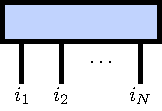
\includegraphics[scale=1]{figures/tikz/Tensor_Networks/basic_diagrams/basic_diagrams_d.pdf}}
	\subcaptionbox{\label{fig:basic_tensor_diagrams_scalar}}
	{%
		\raisebox{\dimexpr.5\ht\largestimage-.5\height}
		{%
			
\includegraphics[scale=1]{figures/tikz/Tensor_Networks/basic_diagrams/basic_diagrams_a.pdf}
		}
	}
	\quad\quad
	\subcaptionbox{\label{fig:basic_tensor_diagrams_vector}}
	{%
		\raisebox{\dimexpr.5\ht\largestimage-.5\height}
		{%
			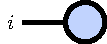
\includegraphics[scale=1]{figures/tikz/Tensor_Networks/basic_diagrams/basic_diagrams_b.pdf}
		}
	}
	\quad\quad
	\subcaptionbox{\label{fig:basic_tensor_diagrams_matrix}}
	{%
		\raisebox{\dimexpr.5\ht\largestimage-.5\height}
		{%
			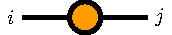
\includegraphics[scale=1]{figures/tikz/Tensor_Networks/basic_diagrams/basic_diagrams_c.pdf}
		}
	}
	\quad\quad
	\subcaptionbox{\label{fig:basic_tensor_diagrams_rank_n_tensor}}
	{%
		\usebox{\largestimage}
	}
\caption{Tensors of different ranks are shown in diagrammatic notation. (a) A scalar, (b) a vector, (c) a matrix, (d) a general tensor of rank $n$ as defined in Equation \eqref{eq:general_tensor_rank_n}.}
\label{fig:basic_tensor_diagrams}
\end{figure}
An \textit{index contraction} between two or more tensors is the linear operation that is performed by summing over a given set of indices. For example, the scalar product of two vectors $A\in\mathbb{C^\chi}$ and $B\in\mathbb{C^\chi}$,
\begin{equation}
	\label{eq:example_tensor_network_scalar_product}
	c = \sum_{\alpha=1}^{\chi}A_\alpha B_\alpha,\quad c\in\mathbb{C},
\end{equation}
and the matrix product of two matrices $A\in\mathbb{C}^{\chi_1\times\chi_2}$, $B\in\mathbb{C}^{\chi_2\times\chi_3}$,
\begin{equation}
	\label{eq:example_tensor_network_matrix_product}
	C_{ij} = \sum_{\alpha=1}^{\chi_2} A_{i\alpha} B_{\alpha j},\quad C\in\mathbb{C}^{\chi_1\times\chi_3}
\end{equation}
constitute index contractions. A more involved example is the index contraction of two rank-3 tensors $A\in\mathbb{C}^{\chi_1\times\chi_2\times\chi_3}$, $B\in\mathbb{C}^{\chi_2\times\chi_4\times\chi_5}$ and one rank-4 tensor $C\in\mathbb{C}^{\chi_3\times\chi_5\times\chi_6\times\chi_7}$, where we contract along the indices with dimension $\chi_2$, $\chi_3$ and $\chi_5$. The result is a rank-4 tensor $D\in\mathbb{C}^{\chi_1\times\chi_4\times\chi_6\times\chi_7}$:
\begin{equation}
	\label{eq:example_tensor_network_involved_network}
	D_{ijkl} = \sum_{\alpha=1}^{\chi_2} \sum_{\beta=1}^{\chi_3} \sum_{\gamma=1}^{\chi_5} A_{i \alpha \beta} B_{\alpha j\gamma} C_{\beta \gamma k l}.
\end{equation}
In tensor diagrams, index contractions are drawn by connecting the legs corresponding to contracted indices. Lines connecting two tensors are sometimes called \textit{bonds}, while indices not used in contractions are called \textit{open indices}. The \textit{bond dimension} $\chi_i$ denotes the number of different values an index $i$ can take. It is often more convenient to discuss tensor network algorithms in terms of diagrams than in terms of equations. \par
A \textit{tensor network} is defined as a set of tensors that is contracted in a specified way. We draw the tensor diagrams of the above equations in Figure \figref{fig:basic_tensor_network_diagrams}.\par
\begin{figure}[h]
	\centering
	% Store largest image in a box
	\savebox{\largestimage}{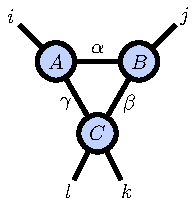
\includegraphics[scale=1]{figures/tikz/Tensor_Networks/basic_networks/basic_networks_c.pdf}}
	\subcaptionbox{\label{fig:basic_tensor_networks_matrix_vector_product}}
	{%
		\raisebox{\dimexpr.5\ht\largestimage-.5\height}
		{%
			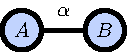
\includegraphics[scale=1]{figures/tikz/Tensor_Networks/basic_networks/basic_networks_a.pdf}
		}
	}
	\subcaptionbox{\label{fig:basic_tensor_networks_matrix_product}}
	{%
		\raisebox{\dimexpr.5\ht\largestimage-.5\height}
		{%
			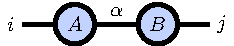
\includegraphics[scale=1]{figures/tikz/Tensor_Networks/basic_networks/basic_networks_b.pdf}
		}
	}
	\subcaptionbox{\label{fig:basic_tensor_networks_involved_contraction}}
	{%
		\usebox{\largestimage}
	}
	\caption{Tensor networks in diagrammatic notation. (a) Scalar product \eqref{eq:example_tensor_network_scalar_product}. (b) Matrix product \eqref{eq:example_tensor_network_matrix_product}. (c) More involved network consisting of three tensors \eqref{eq:example_tensor_network_involved_network}.}
	\label{fig:basic_tensor_network_diagrams}
\end{figure}
Because tensor contractions are linear, the order in which tensors are contracted does not change the result. However, the computational complexity does in general depend on the order of contractions and can thus be minimized by choosing the optimal contraction order. The computational complexity of a tensor contraction of two tensors is simply the product of all bond dimensions, where bond dimensions of contracted indices only appear in the product once. For example, the computational complexity of contracting tensors $B$ and $C$ from the contraction \eqref{eq:example_tensor_network_involved_network} scales as $\mathcal{O}(\chi_1\chi_2\chi_4\chi_5\chi_6\chi_7)$. \par
Given two normed vector spaces $V_1$ and $V_2$ with $\dim\left(V_1\right) = m$, $\dim\left(V_2\right) = n$, $m \le n$, an \textit{isometry} (sometimes also called \textit{semi-unitary}) is a linear, norm-preserving map $W: V_1 \rightarrow V_2$ from the smaller to the larger vector space. Each isometry can be represented by a $n\times m$ matrix $W$ fulfilling the \textit{isometry condition}
\begin{equation}
	\label{eq:isometry_condition_general}
	W^\dagger W = \id, \quad WW^\dagger = \mathbb{P},
\end{equation}
where $\mathbb{P} = \mathbb{P}^2$ is a projection. If $m = n$, it holds $\mathbb{P} = \id$ and $W$ is a \textit{unitary map}. An isometry tensor is a tensor that through grouping of indices and reshaping (i.e. matricization) becomes an isometry. In tensor network diagrams, we draw isometries by decorating lines with arrows. Following the convention of \cite{cite:isometric_tensor_network_states_in_two_dimensions, cite:efficient_simulation_of_dynamics_in_two_dimensional_quantum_spin_systems}, we denote the indices belonging to the larger vector space by incoming arrows and the indices belonging to the smaller vector space by outgoing arrows. Unitary tensors are decorated with bidirectional arrows on all indices, where the grouping must be inferred from the context. Ordinary tensors are drawn without arrows. Tensor diagrams for isometric and unitary tensors are shown in Figure \figref{fig:isometries_and_unitaries_diagrams}.\par
\begin{figure}[h]
	\centering
	\subcaptionbox{\label{fig:basic_isometries_isometric_matrix}}
	{%
		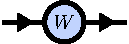
\includegraphics[scale=1]{figures/tikz/Tensor_Networks/basic_isometries/basic_isometries_a.pdf}
	}
	\par\bigskip
	\subcaptionbox{\label{fig:basic_isometries_unitary_matrix}}
	{%
	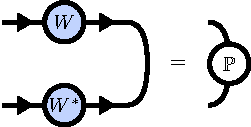
\includegraphics[scale=1]{figures/tikz/Tensor_Networks/basic_isometries/basic_isometries_c.pdf}
	}
	\par\bigskip
	\subcaptionbox{\label{fig:basic_isometries_isometric_tensor}}
	{%
		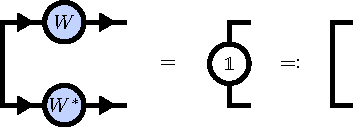
\includegraphics[scale=1]{figures/tikz/Tensor_Networks/basic_isometries/basic_isometries_b.pdf}
	}
	\caption{(a) A isometric matrix $W$ is depicted as a tensor diagram. The isometry condition \eqref{eq:isometry_condition_general} reduces contractions of $W$ with its adjoint to the identity matrix or to a projector $\mathbb{P}$. (b) A unitary matrix $U$ is drawn by using double arrows. For unitary matrices, the projector $\mathbb{P}$ is equal to the identity. (c) Isometric tensors of higher rank must fulfil the isometry condition by grouping of indices.}
	\label{fig:isometries_and_unitaries_diagrams}
\end{figure}
We lastly introduce an inner product for rank-$n$ tensors $A, B \in \mathbb{C}^{\chi_1\times\dots\times\chi_n}$, the \textit{Frobenius inner product}
\begin{equation}
	\label{eq:frobenius_inner_product}
	\left\langle A, B\right\rangle_\text{F} \coloneqq \sum_{\mu_1=1}^{\chi_1} \dots \sum_{\mu_n=1}^{\chi_n} A_{\mu_1\dots\mu_n}^*B_{\mu_1\dots\mu_n} = \Tr\left(A^\dagger B\right),
\end{equation}
where the last equality holds only if $n = 2$. The Frobenius inner product induces a norm, the \textit{Frobenius norm}
\begin{equation}
	\label{eq:frobenius_norm}
	\lVert A\rVert_\text{F} = \sqrt{\left\langle A, A\right\rangle_\text{F}},
\end{equation}
which can be used to define a measure of distance $\lVert A-B\rVert_\text{F}$ between tensors $A$ and $B$.

\newpage
\section{Tensor Decompositions}
\label{sec:tensors_and_tensor_networks_tensor_decompositions}
There are two decompositions that are used extensively in this thesis: The QR-decomposition and the Singular Value Decomposition. Both decompositions are matrix decompositions but can be applied to tensors as well by first grouping indices and reshaping to a matrix, applying the decomposition, and reshaping the result back to the original bond dimensions. \par
The \textit{reduced QR-decomposition} of a matrix $A \in \mathbb{C}^{n\times m}$ is the decomposition
\begin{equation}
	\label{eq:QR_decomposition_general}
	A = QR,
\end{equation}
where $Q\in\mathbb{C}^{n\times k}$ is an isometry, $R\in\mathbb{C}^{k\times m}$ is an upper triangular matrix and $k \coloneqq \min(n, m)$. The computational complexity of the QR decomposition scales as
\begin{equation}
	\label{eq:QR_decomposition_complexity}
	\mathcal{O}\left(n\cdot m\cdot\min(n, m)\right).
\end{equation}
A diagrammatic depiction of the QR decomposition \eqref{eq:QR_decomposition_general} is drawn in figure \figref{fig:tensor_decomposition_diagrams}(a). \par
The \textit{Singular Value Decomposition} (SVD) of a matrix $A \in \mathbb{C}^{n\times m}$ is the decomposition
\begin{equation}
	\label{eq:SVD_general}
	A = USV^\dagger,
\end{equation}
where $U\in\mathbb{C}^{n\times k}$ and $V\in\mathbb{C}^{m\times k}$ are isometries, $S\in\mathbb{R}^{k\times k}$ is a diagonal real matrix of \textit{singular values}, and $k \coloneqq \min(n, m)$. The computational complexity of the SVD is the same as for the QR decomposition \eqref{eq:QR_decomposition_complexity}. However, while the scaling is the same, the prefactors are lower for the QR decomposition in most implementations, meaning that the QR decomposition is faster in practice. Moreover, in contrast to the SVD, the QR decomposition allows for highly efficient implementations on graphics processing units (GPUs), which enables decompositions of large matrices to be carried out significantly faster and more power efficiently. Thus, whenever the singular values are not needed, the QR decomposition is preferred over the SVD. Figure \figref{fig:tensor_decomposition_diagrams} shows a tensor network diagram of the SVD \eqref{eq:SVD_general}. \par
An important property of the SVD is that it can be used to approximate a matrix $A$ by a matrix $\tilde{A}$ of lower rank $\chi < \min(m, n)$. This \textit{truncated SVD} can be performed by keeping only the largest $\chi < k$ singular values and omitting the corresponding columns of $U$ and $V$:
\begin{equation}
	\label{eq:truncated_SVD_general}
	A \approx \tilde{A} = \tilde{U}\tilde{S}\tilde{V},
\end{equation}
with isometries $\tilde{U}\in\mathbb{C}^{n\times\chi}$, $\tilde{V}\in\mathbb{C}^{m\times\chi}$ and real diagonal matrix $\tilde{S}\in\mathbb{C}^{\chi\times\chi}$. It can be shown \cite{cite:eckart_young_theorem} that the truncated SVD minimizes the distance $\lVert A - \tilde{A} \rVert_\text{F}$ between $A$ and $\tilde{A}$ under the constraint $\text{rank}(\tilde{A}) = \chi$. The truncated SVD is frequently used in tensor network algorithms to truncate tensors to a maximum bond dimension $\chi_\text{max}$. \par
\begin{figure}
	\centering
	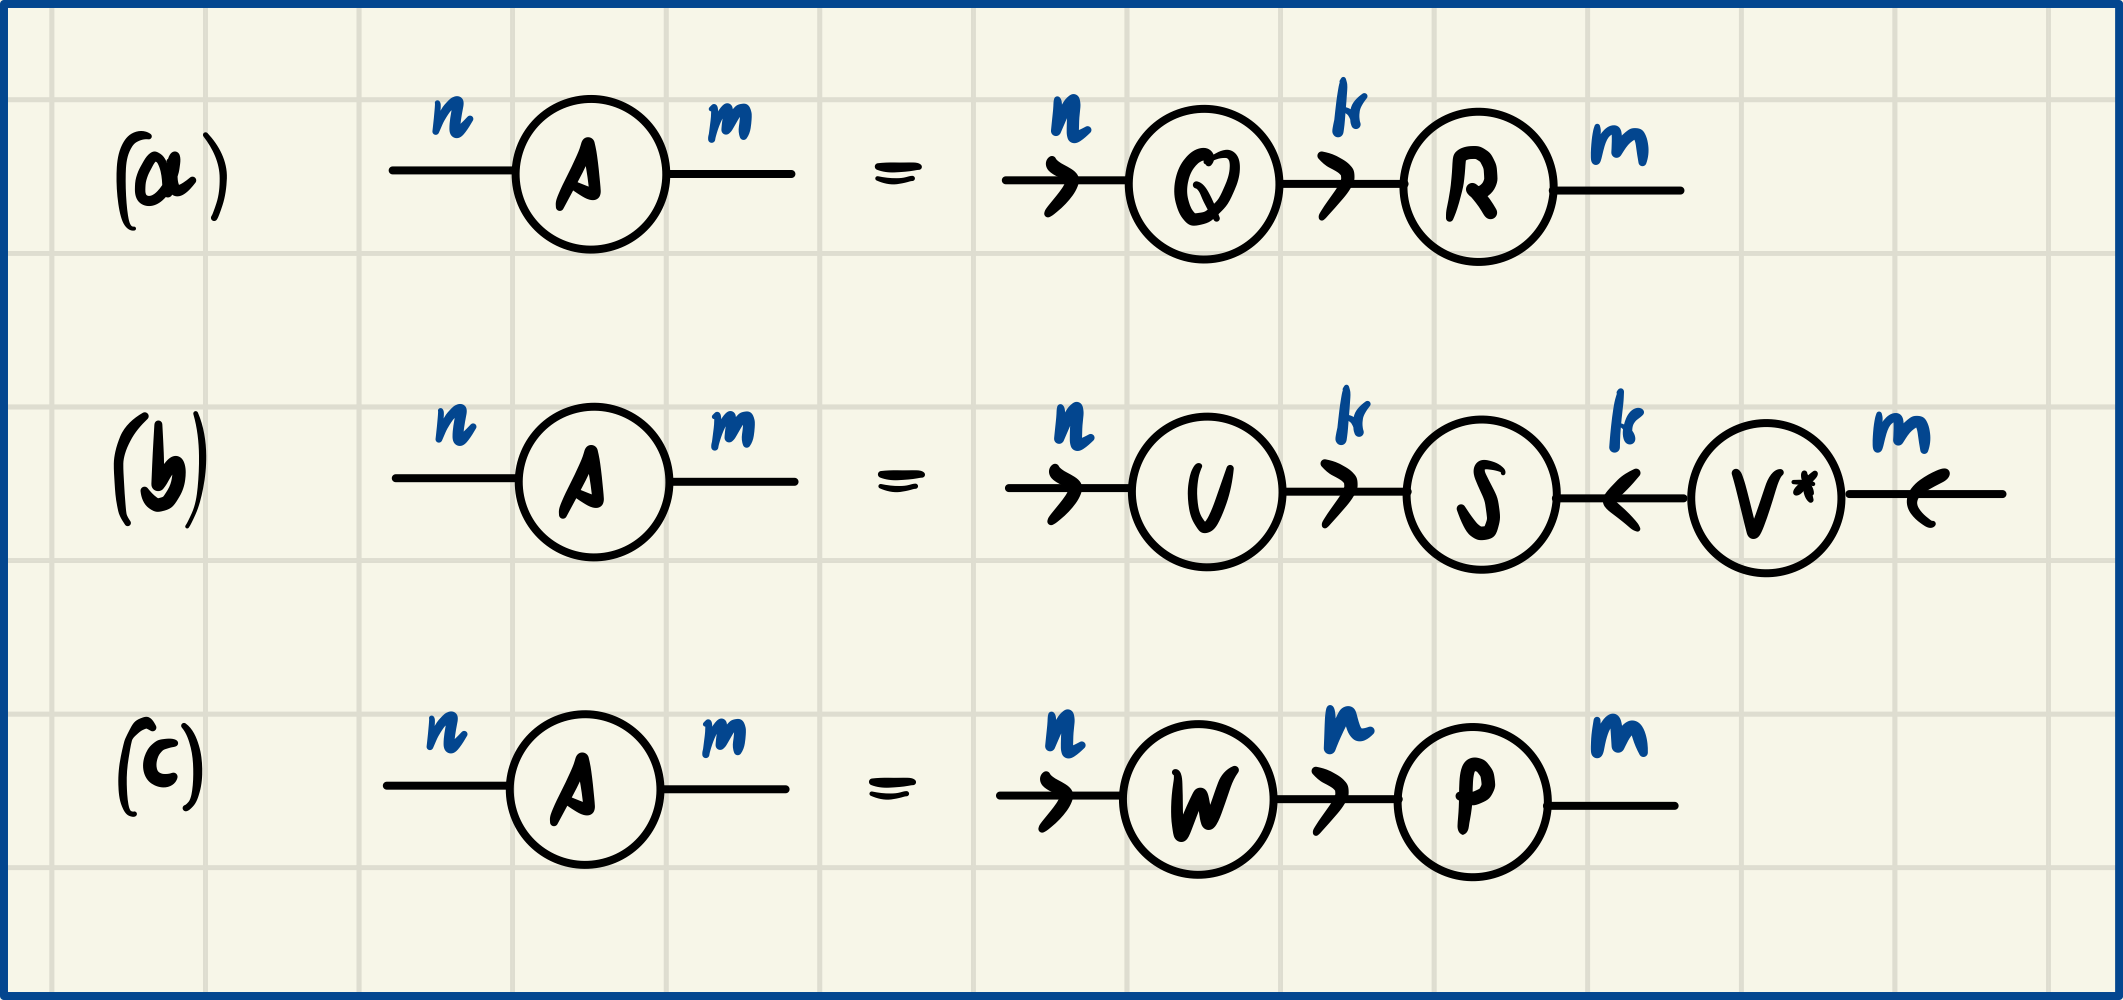
\includegraphics[width=0.8\textwidth]{figures/Tensor_Networks/tensor_decomposition_diagrams.jpeg}
	\caption{Different tensor decompositions are shown in tensor network diagram notation. The indices are decorated with bond dimensions. (a) QR decomposition \eqref{eq:QR_decomposition_general}. (b) Singular Value Decomposition \eqref{eq:SVD_general}}
	\label{fig:tensor_decomposition_diagrams}
\end{figure}
\todo{Discuss error of truncated SVD!}

\section{Isometric Tensor Networks}
\label{sec:tensors_and_tensor_networks_isometric_tensor_networks}
An isometric tensor network is a tensor network whose diagrams bonds can be consistently assigned with arrows. In particular we will look at finite tensor networks where the arrows do not form any loops. In such networks, all arrows point to a single tensor, the \textit{orthogonality center}. These networks have the very useful property that the error of local approximations around the orthogonality center can be computed locally, without contracting the full network. Let $\mathcal{N}$ be the tensor that is the result of contracting the full network, and let $\mathcal{M}$ be the tensor resulting from the contraction of a subregion of the network around the orthogonality center, where all arrows in the tensor network diagram point towards $\mathcal{M}$ (see Figure \figref{fig:isometric_tensor_network_N} for an example in tensor diagram notation). Let us now approximate the sub-network $\mathcal{M}$ by a different sub-network $\mathcal{M}^\prime$, which changes the contraction of the full network to $\mathcal{N}^\prime$ (see \figref{fig:isometric_tensor_network_N_prime}). We can compute the error $\varepsilon$ of this approximation as
\begin{equation}
\begin{split}
	\varepsilon^2 &= \lVert\mathcal{N}-\mathcal{N}^\prime\rVert^2_\text{F} \\
	&=
	\left\langle\mathcal{N}-\mathcal{N}^\prime, \mathcal{N}-\mathcal{N}^\prime\right\rangle_\text{F} \\
	&= \lVert\mathcal{N}\rVert_\text{F}^2 + \lVert\mathcal{N}^\prime\rVert_\text{F}^2 - 2\Re\left\langle\mathcal{N},\mathcal{N}^\prime\right\rangle_\text{F} \\
	&= \lVert\mathcal{M}\rVert_\text{F}^2 + \lVert\mathcal{M}^\prime\rVert_\text{F}^2 - 2\Re\left\langle\mathcal{M},\mathcal{M}^\prime\right\rangle_\text{F} \\
	&= \lVert\mathcal{M}-\mathcal{M}^\prime\rVert^2_\text{F},
\end{split}
\end{equation}
where in the fourth step we used the fact that all tensors outside of the sub-network satisfy the isometry condition. As an example, the contraction of $\langle\mathcal{N},\mathcal{N}^\prime\rangle_\text{F} = \langle\mathcal{M},\mathcal{M}^\prime\rangle_\text{F}$ is shown in Figure \figref{fig:isometric_tensor_network_norm_contraction}. As one can see, the computation of the error reduces to a contraction of the local sub-networks. This greatly simplifies the computation of optimal approximations of tensors especially for large networks because the full network does not need to be contracted. When the tensor network represents a quantum state, this also makes it very easy to compute local expectation values, as will become clear in the next section. This is because the computation of the overlap of the wave function can be simplified to a contraction of a local environment around the orthogonality center. Additionally, approximations made by the truncated SVD \ref{eq:truncated_SVD_general} are, when performed at the orthogonality center, globally optimal for isometric tensor networks, instead of only locally optimal for non-isometric tensor networks.
\begin{figure}
	\centering
	\subcaptionbox{\label{fig:isometric_tensor_network_N}}
	{%
		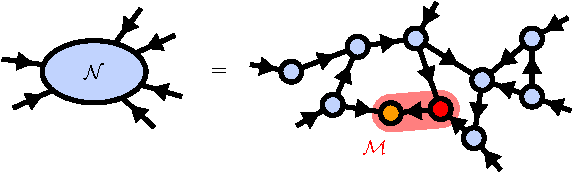
\includegraphics[scale=1]{figures/tikz/Tensor_Networks/contractions_of_isometric_tensor_networks/contractions_of_isometric_tensor_networks_a.pdf}
	}
	\par\bigskip
	\subcaptionbox{\label{fig:isometric_tensor_network_N_prime}}
	{%
		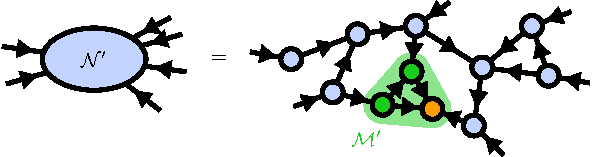
\includegraphics[scale=1]{figures/tikz/Tensor_Networks/contractions_of_isometric_tensor_networks/contractions_of_isometric_tensor_networks_b.pdf}
	}
	\par\bigskip
	\subcaptionbox{\label{fig:isometric_tensor_network_norm_contraction}}
	{%
		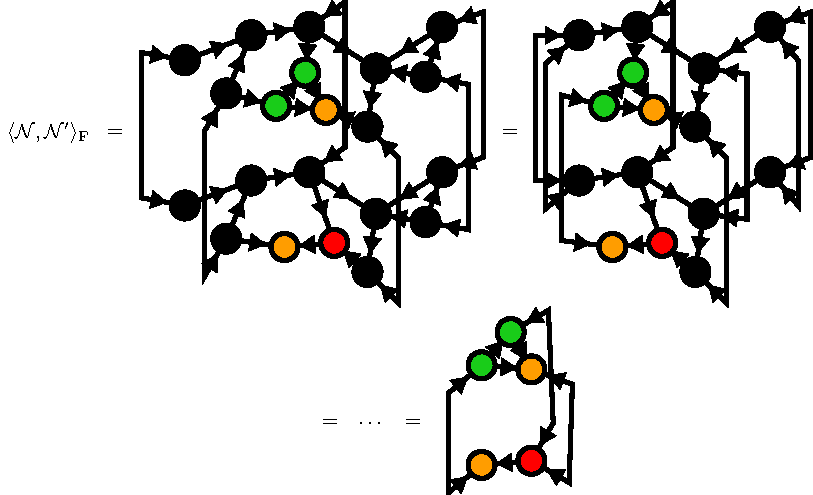
\includegraphics[scale=1]{figures/tikz/Tensor_Networks/contractions_of_isometric_tensor_networks/contractions_of_isometric_tensor_networks_c.pdf}
	}
	\caption{(a) An isometric tensor network $\mathcal{N}$ with the orthogonality center depicted in orange. The sub-network $\mathcal{M}$ is made up of all tensors in the red region. (b) The isometric tensor network $\mathcal{N}^\prime$ with an updated sub-network $\mathcal{M}^\prime$. (c) The computation of the inner product $\langle\mathcal{N},\mathcal{N}^\prime\rangle_\text{F}$ reduces to a contraction of the subregions $\langle\mathcal{M},\mathcal{M}^\prime\rangle_\text{F}$ because of the isometry condition. In the shown tensor network, the tensors of $\mathcal{N}^\prime$ are complex conjugated.}
	\label{fig:isometric_tensor_network_local_approximation}
\end{figure}

\newpage
\section{Matrix Product States (MPS)}
\label{sec:tensors_and_tensor_networks_matrix_product_states}
The Density Matrix Renormalization Group (DMRG) algorithm, a variational method over the class of Matrix Product States (MPS), has developed to be the de-facto standard for the numerical simulation of one-dimensional quantum systems. The success of this method is due to the remarkable ability of MPS to capture the area law entanglement characteristics of ground states of gapped Hamiltonians. Additionally, due to the elegant diagrammatic notation of tensor networks, new algorithms can be developed and discussed efficiently and intuitively. Applications of MPS include finding ground and thermal states, real and imaginary time evolution, and the computation of dynamical properties of lattice Hamiltonians. In the following, we give a brief introduction to MPS, for a more in-depth discussion see \cite{cite:DMRG_in_the_age_of_MPS, cite:practical_introduction_MPS_and_PEPS, cite:tenpy}. \par
The state of a quantum many-body system can be written as
\begin{equation}
	\ket{\Psi} = \sum_{i_1=1}^{d_1} \sum_{i_2=1}^{d_2} \cdots \sum_{i_N=1}^{d_N} \Psi_{i_1,i_2,\dots,i_N} \ket{i_1} \otimes \ket{i_2} \otimes \cdots \otimes \ket{i_N},
\end{equation}
where $N$ is the number of subsystems (e.g. lattice sites or particles), and $\left\{\ket{i_1} \otimes \ket{i_2} \otimes \dots \otimes \ket{i_N}\right\}$, $i_j = 0, \dots, d_j$ is a set of basis vectors of the full many-body Hilbert space
\begin{equation}
	\mathcal{H} = \bigotimes_{j=1}^{N} \mathcal{H}_j,
\end{equation}
with $\dim\left(\mathcal{H}_j\right) = d_j$ the dimension of the local Hilbert space of subsystem $j$. To simplify the notation, we will assume that the dimension of all local subsystems is the same, $d_j = d$. The $d^N$ complex numbers $\Psi_{i_1,i_2,\dots,i_N}$ fully describe the quantum many-body state, and one can think of $\Psi\in\mathbb{C}^{d\times\cdots\times d}$ as a tensor of rank $N$. However, due to the number of parameters scaling exponentially with system size, only very small system sizes are accessible computationally. One can proceed by writing $\Psi$ as a tensor network of tensors of lower rank. A \textit{Matrix Product State} (MPS) is constructed by introducing $N$ rank-3 tensors $T^{[n]}\in\mathbb{C}^{d\times \chi_{n-1}\times \chi_{n}}$ and contracting them in a chain as
\begin{equation}
	\label{eq:MPS_open_boundary_conditions_general_definition}
	\Psi_{i_1,i_2,\cdots,i_N} \coloneqq \sum_{\alpha_1=1}^{\chi_1} \sum_{\alpha_2=1}^{\chi_2}\dots\sum_{\alpha_{N-1}=1}^{\chi_{N-1}}T^{[1],i_1}_{1,\alpha_1} T^{[2],i_2}_{\alpha_1,\alpha_2} \cdots T^{[N],i_N}_{\alpha_{N-1},1},
\end{equation}
where we have written the indices $i_n$ as superscripts, such that the sums are performed only over subscripts. Note that in this notation the bond dimensions at the two ends of the chain are $\chi_0 = \chi_{N} = 1$, and we can interpret the tensors $T^{[1]}$ and $T^{[N]}$ as tensors of rank-2. Since the indices $i_n = 0, 1, \dots d$ represent the local physical degrees of freedom, they are sometimes referred to as \textit{physical indices}. The other indices are called \textit{virtual indices}. A tensor diagram of the MPS \eqref{eq:MPS_open_boundary_conditions_general_definition} is given in Figure \figref{fig:mps_general}.\par
\begin{figure}
	\centering
	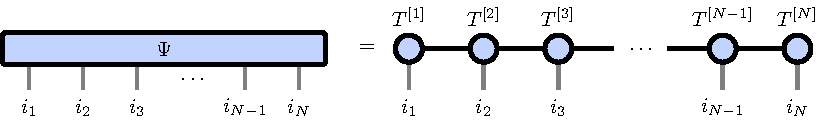
\includegraphics[scale=1]{figures/tikz/Tensor_Networks/mps_basic/mps_basic.pdf}
	\caption{Diagrammatic representation of the Matrix Product State \ref{eq:MPS_open_boundary_conditions_general_definition}.}
	\label{fig:mps_general}
\end{figure}
\begin{figure}
\centering
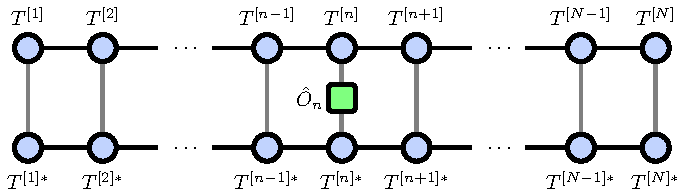
\includegraphics[scale=1]{figures/tikz/Tensor_Networks/mps_local_expectation_value/mps_local_expectation_value.pdf}
\caption{The computation of the expectation value of a local operator can be computed by contracting the MPS with its conjugate transpose, with the operator "sandwiched" in between.}
\label{fig:mps_local_expectation_value}
\end{figure}
An important property of MPS is the existence of a \textit{canonical form} as an isometric tensor network, where a single tensor $T^{[n]} \eqqcolon \Lambda^{[n]}$ is selected as the orthogonality center. One can bring an arbitrary MPS into this canonical form through successive QR-decompositions or SVDs, starting at the outer ends of the chain and isometrizing one tensor at a time, until the orthogonality center is reached \cite{cite:DMRG_in_the_age_of_MPS}. In Figure \figref{fig:mps_canonical_form_general_definition} an MPS in canonical form with the orthogonality center at subsystem $n$ is visualized in diagrammatic notation. We call tensors to the left of the orthogonality center $A^{[i]}$ and tensors to the right of the orthogonality center $B^{[i]}$. The canonical form greatly simplifies many operations on MPS and allows for the formulation of efficient algorithms, where many contractions reduce to identity due to the isometry condition \eqref{eq:isometry_condition_general}, see Figure \figref{fig:mps_left_isometry_condition} and Figure \figref{fig:mps_right_isometry_condition}. For example, the expectation value $\bra{\Psi}\hat{O}\ket{\Psi}$ of a one-site operator $\hat{O} \in \mathbb{C}^{d\times d}$ acting on site $n$ can for a general MPS be computed as
\begin{equation}
\begin{split}
	\label{eq:computation_of_expectation_value_MPS}
	\bra{\Psi}\hat{O}\ket{\Psi} &=\sum_{i_1,\dots,i_N,j_n=1}^{d}\Psi_{i_1,i_2,\dots,i_N} \Psi_{i_1,\dots,i_{n-1},j_n,i_{n+1},\dots,i_N}^* \bra{j_n}\hat{O} \ket{i_n} \\
	&= \sum_{i_1,\dots,i_N,j_n=1}^{d} \left(T^{[1],i_1}\cdots T^{[N],i_N}\right) \\
	&\quad\quad\quad\quad\quad\,\,\cdot\left(T^{[1],i_1*}\cdots T^{[n],j_n*} \cdots T^{[N],i_N*}\right)\cdot \hat{O}_{i_n,j_n},
\end{split}
\end{equation}
where the $T^{[n],i_n}$ are interpreted as matrices for $1 < n < N$ and as row/column vectors for $n = 1, N$ such that the product
\begin{equation}
	\left(T^{[1],i_1}\cdots T^{[N],i_N}\right)
\end{equation}
gives a scalar. The contraction \eqref{eq:computation_of_expectation_value_MPS} is visualized as a tensor diagram in Figure \figref{fig:mps_local_expectation_value}. Here the advantage of the diagrammatic notation becomes appearant: It is much easier to understand how tensors are contracted when expressing the contraction in terms of tensor network diagrams. The computational cost of computing the expectation value scales linear with the system size $\mathcal{O}\left(N\chi^3d\right)$, where $\chi$ is the maximum virtual bond dimension $\chi = \max\left\{\chi_1,\dots,\chi_N\right\}$. If the MPS is however given in canonical form with the orthogonality center at site $n$, the computation reduces to a contraction of only three tensors as can be seen in Figure \figref{fig:mps_local_expectation_value_canonical}, and the computational cost $\mathcal{O}\left(\chi^3d\right)$ becomes independent of system size. \par
\begin{figure}
	\centering
	\begin{minipage}{1.0\textwidth}
		\centering
		\subcaptionbox{\label{fig:mps_canonical_form_general_definition}}
		{%
			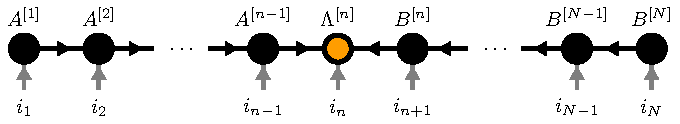
\includegraphics[scale=1]{figures/tikz/Tensor_Networks/mps_canonical_form/mps_canonical_form_a.pdf}
		}
	\end{minipage}
	\par\medskip
	\centering
	\subcaptionbox{\label{fig:mps_left_isometry_condition}}
	{%
		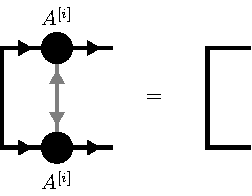
\includegraphics[scale=1]{figures/tikz/Tensor_Networks/mps_canonical_form/mps_canonical_form_b.pdf}
	}
	\quad\quad\quad\quad\quad
	\subcaptionbox{\label{fig:mps_right_isometry_condition}}
	{%
		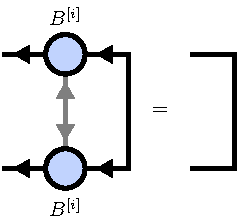
\includegraphics[scale=1]{figures/tikz/Tensor_Networks/mps_canonical_form/mps_canonical_form_c.pdf}
	}
	\caption{(a) Diagrammatic representation of an MPS in canonical form. (b) The left isometry condition. (c) The right isometry condition.}
	\label{fig:mps_canonical}
\end{figure}
\begin{figure}
	\centering
	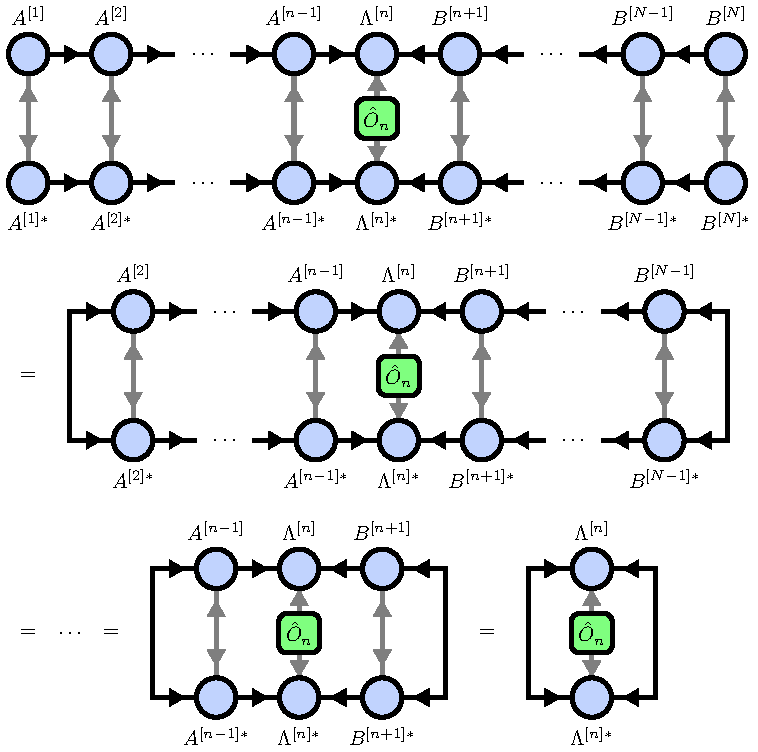
\includegraphics[scale=1.0]{figures/tikz/Tensor_Networks/mps_canonical_form_local_expectation_value/mps_canonical_form_local_expectation_value.pdf}
	\caption{If the MPS is in canonical form, the computation of the expectation value of a local operator can be simplified to a contraction of only three tensors using the isometry condition.}
	\label{fig:mps_local_expectation_value_canonical}
\end{figure}
\subsubsection*{\hspace{95pt}Approximating quantum states with MPS}
Until now, the MPS representation of $\ket{\Psi}$ is still exact. One can approximate an MPS by restricting the virtual bond dimension to a maximal bond dimension $\chi_n < \chi_\text{max}$. In this case, the number of parameters that need to be stored to describe the state is reduced from $\mathcal{O}\left(d^N\right)$ to $\mathcal{O}\left(N\chi_\text{max}^2 d\right)$. To arrive at this approximation, two neighbouring tensors can be contracted and split via a truncated SVD, keeping only the $\chi_\text{max}$ largest singular values. If the orthogonality center of the MPS is at one of the two tensors, this approximation is globally optimal as explained in Section \ref{sec:tensors_and_tensor_networks_isometric_tensor_networks}. Additionally, this SVD at the orthogonality center is related to the Schmidt decomposition of a bipartite system
\begin{equation}
	\ket{\Psi} = \sum_{\alpha=1}^{\chi_n} \lambda_\alpha \ket{\Psi^{[L]}_\alpha} \otimes \ket{\Psi^{[R]}_\alpha},
\end{equation}
where the chain is split into a left and right subsystem, grouping all indices to the left and right of the orthogonality center into orthogonal basis vectors $\ket{\Psi^{[L]}_\alpha}$ and $\ket{\Psi^{[R]}_\alpha}$ respectively. In this case, the Schmidt values $\lambda_\alpha >= 0$ coincide with the singular values \cite{cite:DMRG_in_the_age_of_MPS} and one can compute the Von-Neumann entanglement entropy
\begin{equation}
	S = -\sum_{\alpha=1}^{\chi_n} \lambda_\alpha^2 \log\left(\lambda_\alpha^2\right),
\end{equation}
quantifying the amount of entanglement between the left and right subsystem. If the state is normalized, it additionally holds
\begin{equation}
	\sum_{\alpha=1}^{\chi_n} \lambda_\alpha^2 = 1.
\end{equation}
Thus, how well an MPS of a given bond dimension $\chi_\text{max}$ is able to represent a given quantum state is highly dependent on the Schmidt spectrum $\left\{\lambda_\alpha\right\}$ at the different bipartitions of the chain. If the Schmidt values decrease exponentially, only an exponentially small part of the entanglement structure is truncated and the MPS is a good approximation for the original state. It can be shown \cite{cite:area_law_1D_proof, cite:area_laws_review} that for ground states of local, gapped, one dimensional Hamiltonians there holds an \textit{area law}: The entanglement entropy at arbitrary bipartitions of the chain is bounded by a constant
\begin{equation}
	S \le S_\text{max}, 
\end{equation}
where $S_\text{max}$ is independent of the system size. This is in contrast to the fact that the entanglement of states drawn randomly from the many-body Hilbert space on average exhibits \textit{volume law} scaling
\begin{equation}
	\mathbb{E}\left[S\right] > \min\left(N_L, N_R\right)\log(d),
\end{equation}
where $N_L$ and $N_R$ are the number of subsystems in the left and right bipartition. Hence, ground states of gapped Hamiltonians are very non-generic. Note that the constant $S_\text{max}$ scales with the correlation length of the system, which diverges when approaching critical points. \par
It is immediately clear that truncated MPS by construction exhibit area law entanglement scaling if the local subsystems that are represented by each tensor correspond to physical systems on a 1D chain. The maximal entanglement entropy for a bipartition can be reached when all Schmidt values are equal, i.e. $\lambda_\alpha = 1/\sqrt{\chi_n}$ for $\alpha = 1,\dots\chi_n$, and thus
\begin{equation}
	S \le \log\left(\chi_\text{max}\right)
\end{equation}
for arbitrary bipartitions of the chain. One can conclude that MPS are good approximations for ground states of gapped 1D Hamiltonians away from criticality. \par 
For completeness we note that the truncation of all bonds of an MPS is a highly non-linear optimization problem and the naive algorithm of truncating each bond with an SVD does in general not lead to a minimal error. A variational compression procedure can often be used to obtain a lower error at the same maximum bond dimension $\chi_\text{max}$ \cite{cite:DMRG_in_the_age_of_MPS}. \par
\subsubsection*{\hspace{162pt}Time evolution}
Many algorithms have been formulated in the language of MPS. Most notably, the Density Matrix Renormalization Group (DMRG) algorithm can be used for finding ground states of local lattice Hamiltonians \cite{cite:DMRG_in_the_age_of_MPS}. Time evolution of MPS can be performed with the the Time Evolving Block Decimation (TEBD) algorithm \cite{cite:efficient_simulation_of_1D_quantum_many_body_systems, cite:matrix_product_density_operators_simulation_of_finite_temperature_and_dissipative_systems} or the Time Dependant Variational Principle (TDVP) \cite{cite:time_dependent_variational_principle_for_quantum_lattices, cite:unifying_time_evolution_and_optimization_with_MPS}. In the following, we will briefly discuss TEBD, as this algorithm can be generalized easily to isometric tensor product states of higher dimension, which we will do in Section \ref{sec:YB_isoTPS_TEBD}. \par
Assume that we are given a quantum state $\ket{\Psi}$ in the form of an MPS and a Hamiltonian $\hat{H}$ that can be written as a sum of nearest-neighbour operators $\hat{h}^{[j,j+1]}$,
\begin{equation}
	\hat{H} = \sum_{j = 1}^{N-1} \hat{h}^{[j,j+1]}.
\end{equation}
According to the Schrödinger equation, the state $\ket{\Psi}$ can be evolved in time as
\begin{equation}
	\ket{\Psi(t)} = \hat{U}\left(t\right) \ket{\Psi} = e^{-it\hat{H}} \ket{\Psi},
\end{equation}
where we have set $\hbar = 1$. The time evolution operator $U(t)$ is in general very hard to compute and handle exactly. Thus, $U(t)$ is approximated using a \textit{Suzuki-Trotter decomposition}. We start by decomposing the time evolution into a series of $K$ small time steps $\Delta t = t/K$ as
\begin{equation}
	\hat{U}(t) = e^{-it\hat{H}} = \left(e^{-i\Delta t\hat{H}}\right)^K = \left(\hat{U}(\Delta t)\right)^K.
\end{equation}
Next, we split the Hamiltonian into terms acting on even and odd bonds
\begin{equation}
	\hat{H} = \sum_{j \text{ even}}\hat{h}^{[j, j+1]} + \sum_{j \text{ odd}}\hat{h}^{[j, j+1]} \eqqcolon \hat{H}_\text{even} + \hat{H}_\text{odd}.
\end{equation}
We can then use the \textit{Zassenhaus formula}
\begin{equation}
	e^{\varepsilon(\hat{A}+\hat{B})} = e^{\varepsilon \hat{A}} e^{\varepsilon \hat{B}} e^{-\frac{\varepsilon^2}{2}[\hat{A}, \hat{B}]} e^{\frac{\varepsilon^3}{6}\left(2[\hat{B},[\hat{A},\hat{B}]]+[\hat{A},[\hat{A},\hat{B}]]\right)} \dots
\end{equation}
which can be derived from the Baker-Campbell-Hausdorff formula, to approximate
\begin{equation}
	\label{eq:mps_first_order_tebd}
	\begin{split}
		\hat{U}(\Delta t) &= e^{-i\Delta t\left(\hat{H}_\text{even} + \hat{H}_\text{odd}\right)} = e^{-i\Delta t\hat{H}_\text{even}}e^{-i\Delta t\hat{H}_\text{odd}} + \mathcal{O}\left(\Delta t^2\right) \\
		&= \hat{U}^\text{TEBD1}(\Delta t) + \mathcal{O}\left(\Delta t^2\right).
	\end{split}
\end{equation}
This is called a Suzuki-Trotter decomposition of first order. Since operators acting on even bonds commute with each other, the exponential $e^{-i\Delta tH_\text{even}}$ factorizes,
\begin{equation}
	e^{-i\Delta t\hat{H}_\text{even}} = e^{-i\Delta t\sum_{j \text{ even}} \hat{h}^{[j, j+1]}} = \prod_{j \text{ even}} e^{-i\Delta t \hat{h}^{[j, j+1]}},
\end{equation}
and the same holds for the exponential $e^{-i\Delta t\hat{H}_\text{odd}}$. Each bond operator $\hat{U}^{[j, j+1]} \coloneqq e^{-i\Delta t \hat{h}^{[j, j+1]}}$ acting on the combined Hilbert space of sites $j$ and $j+1$ can be reshaped into a tensor of rank 4. The application of the operator $\hat{U}^\text{TEBD1}(\Delta t)$ to a state in MPS form can then be written as the tensor network in Figure \figref{fig:mps_tebd_first_order_overview}.
To perform a single TEBD iteration corresponding to a time evolution of $\Delta t$, we want to approximate this tensor network by a new MPS. This can be done by moving the orthogonality center from left to right, applying the bond operators $\hat{U}^{[j, j+1]}$ while keeping the MPS structure. The process of applying a single bond operator is shown in Figure \figref{fig:mps_tebd_first_order_applying_bond_op}. First, the orthogonality center is moved to site $j$. The two site tensors $\Lambda^{[j]}$ and $B^{[j+1]}$ are then contracted with the bond operator $\hat{U}^{[j, j+1]}$ into a single tensor $\theta$, which is subsequently split and truncated using an SVD. By sweeping twice across the MPS, first applying the bond operators on all even bonds and then the bond operators on all odd bonds, we perform a full TEBD iteration. There exist two sources of errors, the truncation error of the truncated SVD and the error of the Suzuki-Trotter decomposition. The truncation error can be controlled by choosing a larger bond dimension $\chi$, allowing the representation of more entanglement and thus the evolution to larger times. However, generally the amount of entanglement grows exponentially in time \cite{cite:DMRG_in_the_age_of_MPS}, necessitating an exponentially growing bond dimension and practically limiting the algorithm to small times. A smaller Suzuki-Trotter error can be achieved by choosing smaller time steps $\Delta t$ or by performing a higher-order Suzuki-Trotter decomposition. For example, a second order decomposition can be computed by symmetrizing two first-order decompositions of time step $\Delta t /2$ as
\begin{equation}
	\begin{split}
		\hat{U}(\Delta t) &= e^{-i\Delta t\left(\hat{H}_\text{even} + \hat{H}_\text{odd}\right)} = e^{-i\frac{\Delta t}{2}\hat{H}_\text{even}} e^{-i\Delta t \hat{H}_\text{odd}} e^{-i\frac{\Delta t}{2}\hat{H}_\text{even}} + \mathcal{O}\left(\Delta t^3\right)\\
		&= \hat{U}^\text{TEBD2}(\Delta t) + \mathcal{O}\left(\Delta t^3\right).
	\end{split}
\end{equation}
and can be applied to an MPS similarly as the first order decomposition. For higher order Suzuki-Trotter decompositions see \cite{cite:finding_exponential_product_formulas_of_higher_orders}.
\begin{figure}
	\centering
	\subcaptionbox{\label{fig:mps_tebd_first_order_overview}}
	{%
		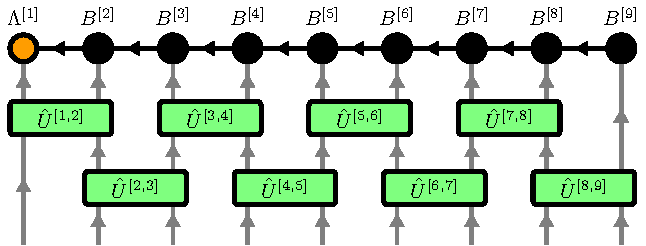
\includegraphics[scale=1]{figures/tikz/Tensor_Networks/mps_TEBD/mps_TEBD_a.pdf}
	}
	\par\medskip
	\subcaptionbox{\label{fig:mps_tebd_first_order_applying_bond_op}}
	{%
		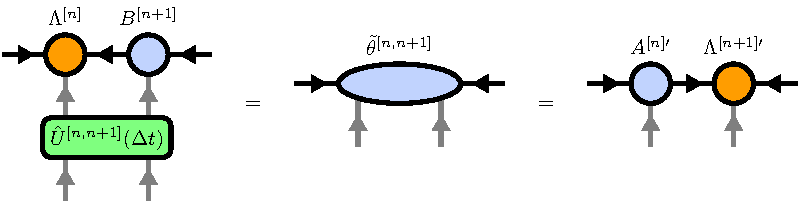
\includegraphics[scale=1]{figures/tikz/Tensor_Networks/mps_TEBD/mps_TEBD_b.pdf}
	}
	\caption{(a) An MPS can be approximately evolved by a time $\Delta t$ by applying the first order TEBD operator \eqref{eq:mps_first_order_tebd}, which is made up of bond operators acting first on all even and then on all odd bonds. (b) To apply a single bond operator $\hat{U}^{[n, n+1]}$, the two corresponding tensors $\Lambda^{[n]}$ and $B^{[n+1]}$ are contracted with the operator into a tensor $\theta^{[n,n+1]}$, which is then split using truncated SVD to obtain the updated tensors $A^{[n]\prime}$ and $\Lambda^{[n+1]^\prime}$.}
	\label{fig:mps_tebd_first_order}
\end{figure}

\section{Isometric Tensor Product States (isoTPS) in 2D}
\label{sec:tensors_and_tensor_networks_isometric_tensor_product_states_in_2D}
The natural generalization of MPS to higher dimensional lattices is given by \textit{Projected Entangled Pair States} (PEPS). A PEPS is constructed similar to a MPS by representing the local subsystem on each lattice site $i$ with the index $\sigma_i$ of a tensor $T_i^{\sigma_i}$ and connecting nearest-neighbour tensors with virtual bonds. The quantum state can then be written as
\begin{equation}
	\label{eq:PEPS_definition_general}
	\left|\Psi\right\rangle = \sum_{\sigma_1,\sigma_2,\dots,\sigma_N} \mathcal{C}\left(T_1^{\sigma_1}, T_2^{\sigma_2}, \dots, T_N^{\sigma_N}\right) \left|\sigma_1,\sigma_2,\dots,\sigma_N\right\rangle,
\end{equation}
where $\mathcal{C}(\dots)$ denotes the contraction of the full network along all virtual bonds. As an example, we draw a PEPS on a square lattice in figure \figref{fig:square_PEPS}. \par
\begin{figure}
	\centering
	\subcaptionbox{\label{fig:square_PEPS}}
	{%
		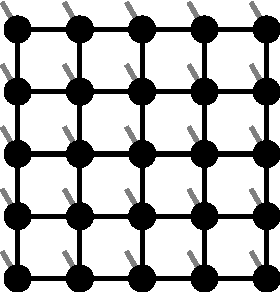
\includegraphics[scale=1]{figures/tikz/Tensor_Networks/isoTPS_structure/isoTPS_structure_a.pdf}
	}
	\quad\quad
	\subcaptionbox{\label{fig:square_isoTPS}}
	{%
		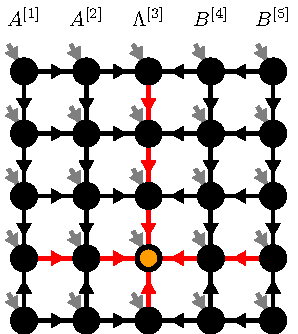
\includegraphics[scale=1]{figures/tikz/Tensor_Networks/isoTPS_structure/isoTPS_structure_b.pdf}
	}
	\caption{Tensor Networks representing two dimensional states on a square lattice. (a) A Projected Entangled Pair State (PEPS). (b) An isometric Tensor Product State (isoTPS). \todo{Include orthogonality center tensor}}
	\label{fig:square_PEPS_and_isoTPS}
\end{figure}
PEPS are able to efficiently represent area-law states in two and higher dimensions \cite{cite:practical_introduction_MPS_and_PEPS}. Remarkably, PEPS can even handle correlations decaying polynomially with separation distance \cite{cite:criticality_the_area_law_and_the_computational_power_of_PEPS}, whereas MPS can only handle exponentially decaying correlations. Polynomially decaying correlations are characteristic for critical points. \par
Unfortunately, it is not generally possible to bring a PEPS into an exact canonical form due to the presence of closed loops. Thus, already the computation of local expectation values scales exponentially with system size and can in practice be only done approximately, e.g. using the boundary MPS method \cite{cite:practical_introduction_MPS_and_PEPS} or corner transfer matrices \cite{cite:CTMRG}. Moreover, algorithms for ground state search and time evolution have computational costs scaling with high powers of the bond dimension. For example the cost of a full update TEBD or DMRG iteration is dominated by the contraction of an effective environment, scaling as $\mathcal{O}\left(D^{10}\right)$ \cite{cite:unifying_PEPS_contractions}. \par
Recently, the new class of \textit{isometric Tensor Product States} (isoTPS) has been introduced \cite{cite:isometric_tensor_network_states_in_two_dimensions, cite:conversion_of_PEPS_into_a_canonical_form, cite:DMRG_approach_to_optimizing_2D_tensor_networks}, generalizing the canonical form of MPS to higher dimensions by enforcing isometry constraints. This allows for efficient computation of local expectation values and greatly lowers the cost of some algorithms. The downside to this approach is that the set of states representable by isoTPS is smaller than the set of state representable by PEPS. It is thus an interesting question to ask which kinds of states and, more generally, which kinds of quantum phases can still be represented by isoTPS. \par
In the following, we will give a brief introduction to the isoTPS defined in \cite{cite:isometric_tensor_network_states_in_two_dimensions} and discuss their properties. A two-dimensional isoTPS on the square lattice is constructed by enforcing the isometry conditions shown in figure \figref{fig:square_isoTPS}. All isometries are chosen in such a way that all arrows point towards a special row and column, called the \textit{orthogonality hypersurface} of the isoTPS. The term "hypersurface" is chosen in anticipation of a generalization to higher dimensions. Because of the isometry condition, one can think of the contractions of each of the four regions outside the orthogonality hypersurface as orthogonal boundary maps \cite{cite:efficient_simulation_of_dynamics_in_two_dimensional_quantum_spin_systems}. The single tensor with only incoming arrows is called the \textit{orthogonality center}. local expectation values of operators acting in the vicinity of the orthogonality center can be computed efficiently because most contractions reduce to identity, similar to the computation of local expectation values in MPS (see figure \figref{fig:mps_local_expectation_value_canonical}). The orthogonality center can be moved along the orthogonality hypersurface simply and exactly using a QR-decomposition as shown in figure \figref{fig:isoTPS_moving_ortho_center}. \par
\begin{figure}
	\centering
	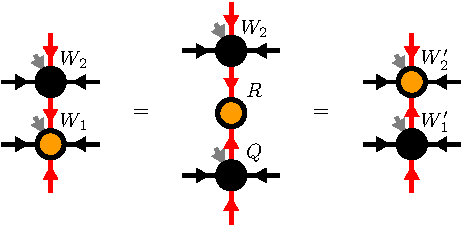
\includegraphics[scale=1]{figures/tikz/Tensor_Networks/isoTPS_moving_ortho_center/isoTPS_moving_ortho_center.pdf}
	\caption{Moving the orthogonality center and the orthogonality hyper surface around is a central problem in isoTPS applications. (a) Moving the orthogonality center along the orthogonality hypersurface can be done easily via QR-decompositions. (b) An orthogonality column can be moved by first solving equation \eqref{eq:isoTPS_moving_ortho_surface_auxillary_formulation} variationally and then absorbing $\Lambda$ into $B_{l+1}$ via the standard MPO-MPS multiplication and MPS compression algorithms.}
	\label{fig:isoTPS_moving_ortho_center}
\end{figure}
\begin{figure}
	\centering
	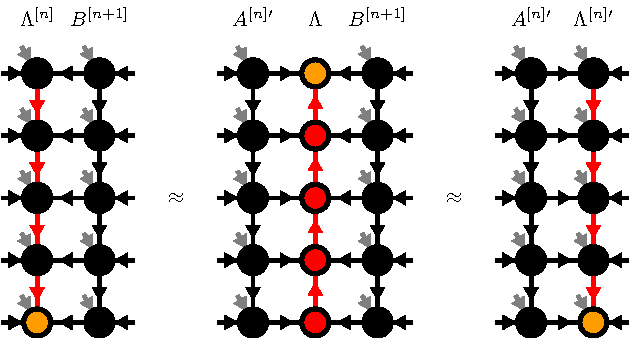
\includegraphics[scale=1]{figures/tikz/Tensor_Networks/isoTPS_moving_ortho_surface/isoTPS_moving_ortho_surface.pdf}
	\caption{The orthogonality hypersurface can be moved to the right by first solving equation \eqref{eq:isoTPS_moving_ortho_surface_auxillary_formulation} variationally and then absorbing $\Lambda$ into $B^{[n+1]}$ via the standard MPO-MPS multiplication and MPS compression algorithms.}
	\label{fig:isoTPS_moving_ortho_column}
\end{figure}
Moving the orthogonality surface is a harder problem, which in general can only be done approximately. In analogy to MPS and as shown in figure \figref{fig:square_isoTPS}, we call columns left of the orthogonality hypersurface $A_l$ and tensors right of the orthogonality hypersurface $B_l$, with $l = 1,2,\dots,L$ and $L$ the linear system size. Moving the orthogonality hypersurface $\Lambda_l$ one column to the right can be expressed as solving the problem
\begin{equation}
	\label{eq:isoTPS_moving_ortho_surface_general}
	\Lambda_l B_{l+1} = A_l \Lambda_{l+1},
\end{equation}
where the notation $\Lambda_l B_{l+1}$ means the contraction of columns $\Lambda_l$ and $B_{l+1}$ along their connecting bonds. Instead of \eqref{eq:isoTPS_moving_ortho_surface_general}, one can solve the simpler auxillary problem
\begin{equation}
	\label{eq:isoTPS_moving_ortho_surface_auxillary_formulation}
	\Lambda_l = A^l \Lambda,
\end{equation}
where $\Lambda$ is a column of tensors with no physical indices, as shown in figure \figref{fig:isoTPS_moving_ortho_column}. This column can then be absorbed into $B_{l+1}$ via the standard algorithm of applying an MPO to an MPS and subsequent MPS compression \cite{cite:DMRG_in_the_age_of_MPS}. One can variationally solve problem \eqref{eq:isoTPS_moving_ortho_surface_auxillary_formulation} by minimizing the distance $\left\lvert\Lambda_l-A_l\Lambda\right\rvert$, sweeping back and forth through the tensors while respecting the isometry condition.\todo{Maybe reference Evenbly-Vidal here?}
\begin{figure}
	\centering
	\subcaptionbox{\label{fig:Moses_move}}
	{%
		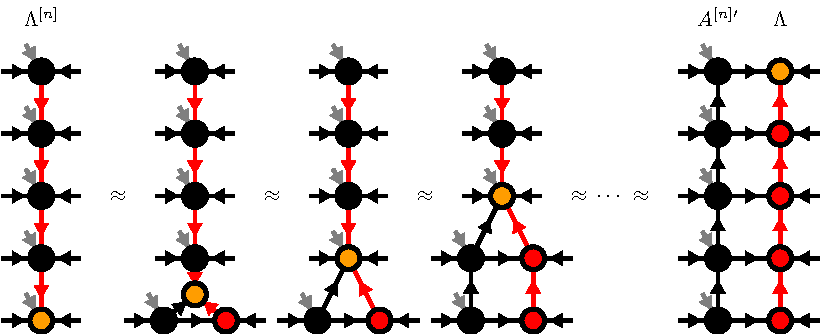
\includegraphics[scale=1]{figures/tikz/Tensor_Networks/isoTPS_MM/isoTPS_MM_a.pdf}
	}
	\subcaptionbox{\label{fig:tripartite_decomposition}}
	{%
		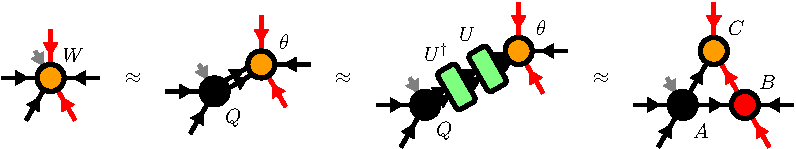
\includegraphics[scale=1]{figures/tikz/Tensor_Networks/isoTPS_MM/isoTPS_MM_b.pdf}
		
	}
	\caption{(a) The Moses Move (MM) splits the column $\Lambda_l$ into $A_l$ and $\Lambda$ via a single unzipping sweep of tripartite decompositions. (b) Tripartite decomposition of the tensor $W$ as explained in the text.}
	\label{fig:Moses_move_and_tripartite_decomposition}
\end{figure}
It is however found in \cite{cite:isometric_tensor_network_states_in_two_dimensions} that a single unzipping sweep, called the \textit{Moses Move} (MM), provides a solution very close to the variational one whilst being far quicker. The MM can also be used as a good initialization for the variational algorithm. We sketch the MM in figure \figref{fig:Moses_move}. We start from the bottom of the orthogonality hypersurface column and split the tensors one after the other using a tripartite decomposition. A single tripartite decomposition of a tensor $W$ is shown in figure \figref{fig:tripartite_decomposition}. First, $W$ is split into two tensors $A$ and $B$ via a truncated SVD $W = U(SV) = AB$ with $A$ an isometry. The bond connecting A and B is reshaped into two bonds. Next, it is important to note that the full contraction is invariant under the insertion of a unitary and its conjugate transpose, $AB = (AU^\dagger)(UB)$, with $(AU^\dagger)$ still satisfying the isometry condition. This degree of freedom can be used to \textit{disentangle} the tensor $B$ along the direction of the red bonds. Accordingly, we choose $U$ such that the truncation error or some entanglement measure is minimized for splits along the direction of the red bonds. Choosing a good disentangling unitary is crucial for a successful tripartite decomposition and will be discussed further in section \ref{sec:}. Assume for now that a good disentangling unitary has been found. After contracting $(AU^\dagger)$ and $(UB)$, a truncated SVD is used to split $(UB)$ into tensors $B^\prime$ and $C^\prime$ as shown in figure \figref{fig:tripartite_decomposition}, completing the tripartite decomposition. \par
Because the orthogonality center can be moved easily along the orthogonality hypersurface, one can think of the orthogonality hypersurface along a column or row as a 1D MPS with an enlarged physical bond dimension grouping together the phsical and the two ancilla legs pertruding from the orthogonality hypersurface tensors. Standard MPS algorithms can then be generalized to isoTPS by performing one iteration of the algorithm on the orthogonality hypersurface MPS, before moving the hypersurface via MM or variational optimization and repeating the procedure. As an example, we will discuss TEBD$^2$, the generalization of $TEBD$ to an isoTPS on a 2D square lattice. \todo{write}. \par
isoTPS are a new class of states that enable the implementation of faster algorithms for e.g. ground state search and time evolution, compared to PEPS. The expressional power of isoTPS has been studied in \cite{cite:isometric_tensor_network_representation_of_string_net_liquids}, where it was found that isoTPS with finite bond dimension can exactly represent ground state wavefunctions of string-net liquid models, showing that long-range entanglement does not form an obstruction for isoTPS representations and suggesting that the ground states of gapped Hamiltonians with gappable edges can be efficiently represented as an isoTPS. There have also been works discussing the computational complexity of isoTNS \cite{cite:computational_complexity_of_isometric_tensor_network_states} and relating isoTNS to quantum circuits \cite{cite:sequential_generation_of_projected_entangled_pair_states, cite:quantum_circuits_for_2D_isometric_tensor_networks}. In \cite{cite:topological_quantum_phase_transitions_in_2D_isometric_tensor_networks}, topological phase transitions were studied with isoTPS, showing that isoTPS can represent some critical states with power-law correlations. A DMRG$^2$-algorithm was implemented on isoTPS in \cite{cite:efficient_simulation_of_dynamics_in_two_dimensional_quantum_spin_systems} and used to compute dynamical structure factors of ground states using real time evolution. IsoTPS were also extended to fermionic systems \cite{cite:fermionic_isometric_tensor_network_states}, to two dimensional strips of infinite length \cite{cite:two_dimensional_isometric_tensor_networks_on_infinite_strip}, and to three dimensional cubic lattices \cite{cite:three_dimensional_isometric_tensor_networks}. They have also been used to compute properties of two dimensional thermal states \cite{cite:isometric_tensor_network_representation_of_2D_thermal_states}.
	
	\chapter{diagonal isometric Tensor Product States (disoDTPS)}
	In the following we introduce a new class of isometric tensor tensor states which we call \textit{diagonal isometric tensor product states} (disoTPS). This class of tensor product states is in many ways similar to the isometric tensor product states discussed in section \ref{sec:tensors_and_tensor_networks_isometric_tensor_product_states_in_2D}, with some important differences. 

\section{Network Structure}
\label{sec:disoTPS_network_structure}
\documentclass[crop,tikz,convert={outext=.svg,command=\unexpanded{pdf2svg \infile\space\outfile}},multi=false]{standalone}
% This file is used to globally define colors, line widths, etc. for diagrams used in the thesis
\usepackage{tikz}
\usepackage{ifthen}

% Libraries
\usetikzlibrary{decorations.markings}
\usetikzlibrary{arrows}

% Basic colors
\definecolor{borderColor}{rgb}{0.0, 0.0, 0.0}
\definecolor{physicalTensorColor}{rgb}{0.757, 0.827, 0.996}
\definecolor{auxillaryTensorColor}{rgb}{1.0, 0.0, 0.0}
\definecolor{orthogonalityCenterColor}{rgb}{1.0, 0.616, 0.0}
\definecolor{physicalLegColor}{rgb}{0.5, 0.5, 0.5}
\definecolor{auxillaryLegColor}{rgb}{1.0, 0.0, 0.0}
\definecolor{virtualLegColor}{rgb}{0.0, 0.0, 0.0}
\definecolor{generalTensorColor}{rgb}{0.757, 0.827, 0.996}
\definecolor{identityColor}{rgb}{1.0, 1.0, 1.0}
<<<<<<< HEAD
<<<<<<< HEAD
\definecolor{redMarkingColor}{rgb}{1.0, 0.0, 0.0}
\definecolor{greenMarkingColor}{rgb}{0.1, 0.8, 0.1}

% Basic sizes
\def \defaultTensorWidth {19pt}
\def \smallTensorWidth {10pt}
=======

% Basic sizes
\def \defaultTensorWidth {19pt}
>>>>>>> 4d788c9927566585e0e5d97c0548041c106e9b2d
=======

% Basic sizes
\def \defaultTensorWidth {19pt}
>>>>>>> 4969d80c4885b9e0e0312ae168d2124e3f884353
\def \defaultLineWidth {2}
\def \xOffsetUnitCell {180pt}
\def \yOffsetUnitCell {180pt}
\def \yOffsetPhysicalLeg {30pt}
\def \defaultArrowscale {0.7}
\def \defaultArrowXShift {7pt}
\def \defaultTextOffset {6pt}
\def \defaultDistanceNormal {40pt}
\def \defaultDistanceEquations {30pt}
\def \identityLegDistance {10 pt}
<<<<<<< HEAD
<<<<<<< HEAD
\def \backgroundopacity {0.5}
=======
>>>>>>> 4d788c9927566585e0e5d97c0548041c106e9b2d
=======
>>>>>>> 4969d80c4885b9e0e0312ae168d2124e3f884353

% Tensor styles
\tikzstyle{tensorPhysical} = [circle, minimum size=\defaultTensorWidth, line width=\defaultLineWidth, fill=physicalTensorColor, draw=borderColor, outer sep=0]
\tikzstyle{tensorAuxillary} = [circle, minimum size=\defaultTensorWidth, line width=\defaultLineWidth, fill=auxillaryTensorColor, draw=borderColor, outer sep=0]
\tikzstyle{tensorOrthoCenter} = [circle, minimum size=\defaultTensorWidth, line width=\defaultLineWidth, fill=orthogonalityCenterColor, draw=borderColor, outer sep=0]

% Leg styles
\tikzstyle{auxillaryLeg} = [color=auxillaryLegColor, line width=\defaultLineWidth, decoration={markings, mark=at position 0.5 with {\pgftransformscale{\defaultArrowscale}\arrow[xshift=\defaultArrowXShift]{triangle 60}}}, postaction={decorate}]
\tikzstyle{physicalLeg} = [color=physicalLegColor, line width=\defaultLineWidth, decoration={markings, mark=at position 0.5 with {\pgftransformscale{\defaultArrowscale}\arrow[xshift=\defaultArrowXShift]{triangle 60}}}, postaction={decorate}]
\tikzstyle{virtualLeg} = [color=virtualLegColor, line width=\defaultLineWidth, decoration={markings, mark=at position 0.5 with {\pgftransformscale{\defaultArrowscale}\arrow[xshift=\defaultArrowXShift]{triangle 60}}}, postaction={decorate}]
\tikzstyle{virtualLegLateArrows} = [color=virtualLegColor, line width=\defaultLineWidth, decoration={markings, mark=at position 0.8 with {\pgftransformscale{\defaultArrowscale}\arrow[xshift=\defaultArrowXShift]{triangle 60}}}, postaction={decorate}]
\tikzstyle{virtualLegWithoutArrows} = [color=virtualLegColor, line width=\defaultLineWidth]
\tikzstyle{physicalLegWithoutArrows} = [color=physicalLegColor, line width=\defaultLineWidth]

% special symbols
\usepackage{amssymb}
\DeclareMathAlphabet{\mathbbb}{U}{bbold}{m}{n}
\newcommand{\id}{\mathbbb{1}}
\newcommand{\iu}{\mathrm{i}}% imaginary unit number i
\newcommand{\Stiefel}{\text{St}(n,p)}


% Layers
\pgfdeclarelayer{bg} % declare background layer
\pgfsetlayers{bg,main} % set order of layers¸

% Command for drawing convex hulls
\newcommand{\convexhull}[2]{
	[   
	create hullnodes/.code={
		\global\edef\namelist{#1}
		\foreach [count=\counter] \nodename in \namelist {
			\global\edef\numberofnodes{\counter}
			\node at (\nodename) [draw=none,name=hullnode\counter] {};
		}
		\node at (hullnode\numberofnodes) [name=hullnode0,draw=none] {};
		\pgfmathtruncatemacro\lastnumber{\numberofnodes+1}
		\node at (hullnode1) [name=hullnode\lastnumber,draw=none] {};
	},
	create hullnodes
	]
	($(hullnode1)!#2!-90:(hullnode0)$)
	\foreach [
	evaluate=\currentnode as \previousnode using \currentnode-1,
	evaluate=\currentnode as \nextnode using \currentnode+1
	] \currentnode in {1,...,\numberofnodes} {
		-- ($(hullnode\currentnode)!#2!-90:(hullnode\previousnode)$)
		let \p1 = ($(hullnode\currentnode)!#2!-90:(hullnode\previousnode) - (hullnode\currentnode)$),
		\n1 = {atan2(\y1,\x1)},
		\p2 = ($(hullnode\currentnode)!#2!90:(hullnode\nextnode) - (hullnode\currentnode)$),
		\n2 = {atan2(\y2,\x2)},
		\n{delta} = {-Mod(\n1-\n2,360)}
		in 
		{arc [start angle=\n1, delta angle=\n{delta}, radius=#2]}
	}
	-- cycle
}
\begin{document}
	\def\tensorDistance{\defaultDistanceSmallDiagonal}
	\def\physicalLegLength{\physicalLegLengthSmall}
	\begin{tikzpicture}
		% Physical tensors
		\node[tensorPhysicalSmall] (T000) at (0, 0) {};
		\node[tensorPhysicalSmall] (T010) at (0, 2*\tensorDistance) {};
		\node[tensorPhysicalSmall] (T020) at (0, 4*\tensorDistance) {};
		
		\node[tensorPhysicalSmall] (T001) at (\tensorDistance, \tensorDistance) {};
		\node[tensorPhysicalSmall] (T011) at (\tensorDistance, 3*\tensorDistance) {};
		\node[tensorPhysicalSmall] (T021) at (\tensorDistance, 5*\tensorDistance) {};
		
		\node[tensorPhysicalSmall] (T100) at (2*\tensorDistance, 0) {};
		\node[tensorPhysicalSmall] (T110) at (2*\tensorDistance, 2*\tensorDistance) {};
		\node[tensorPhysicalSmall] (T120) at (2*\tensorDistance, 4*\tensorDistance) {};
		
		\node[tensorPhysicalSmall] (T101) at (3*\tensorDistance, \tensorDistance) {};
		\node[tensorPhysicalSmall] (T111) at (3*\tensorDistance, 3*\tensorDistance) {};
		\node[tensorPhysicalSmall] (T121) at (3*\tensorDistance, 5*\tensorDistance) {};
		
		\node[tensorPhysicalSmall] (T200) at (4*\tensorDistance, 0) {};
		\node[tensorPhysicalSmall] (T210) at (4*\tensorDistance, 2*\tensorDistance) {};
		\node[tensorPhysicalSmall] (T220) at (4*\tensorDistance, 4*\tensorDistance) {};
		
		\node[tensorPhysicalSmall] (T201) at (5*\tensorDistance, \tensorDistance) {};
		\node[tensorPhysicalSmall] (T211) at (5*\tensorDistance, 3*\tensorDistance) {};
		\node[tensorPhysicalSmall] (T221) at (5*\tensorDistance, 5*\tensorDistance) {};		
		
		% Auxillary tensors
		\node[tensorAuxillarySmall] (W0) at (2.5*\tensorDistance, 0.5*\tensorDistance) {};
		\node[tensorOrthoCenterSmall] (W1) at (2.5*\tensorDistance, 1.5*\tensorDistance) {};
		\node[tensorAuxillarySmall] (W2) at (2.5*\tensorDistance, 2.5*\tensorDistance) {};
		\node[tensorAuxillarySmall] (W3) at (2.5*\tensorDistance, 3.5*\tensorDistance) {};
		\node[tensorAuxillarySmall] (W4) at (2.5*\tensorDistance, 4.5*\tensorDistance) {};
		
		
		\begin{pgfonlayer}{bg}
			% virtual legs
			\draw[virtualLegSmall] (T000) -- (T001);
			\draw[virtualLegSmall] (T010) -- (T011);
			\draw[virtualLegSmall] (T020) -- (T021);
			\draw[virtualLegSmall] (T100) -- (W0);
			\draw[virtualLegSmall] (T110) -- (W2);
			\draw[virtualLegSmall] (T120) -- (W4);
			\draw[virtualLegSmall] (T101) -- (W0);
			\draw[virtualLegSmall] (T111) -- (W2);
			\draw[virtualLegSmall] (T121) -- (W4);
			\draw[virtualLegSmall] (T201) -- (T200);
			\draw[virtualLegSmall] (T211) -- (T210);
			\draw[virtualLegSmall] (T221) -- (T220);
			
			\draw[virtualLegSmall] (T010) -- (T001);
			\draw[virtualLegSmall] (T020) -- (T011);
			\draw[virtualLegSmall] (T110) -- (W1);
			\draw[virtualLegSmall] (T120) -- (W3);
			\draw[virtualLegSmall] (T101) -- (W1);
			\draw[virtualLegSmall] (T111) -- (W3);
			\draw[virtualLegSmall] (T201) -- (T210);
			\draw[virtualLegSmall] (T211) -- (T220);
			
			\draw[virtualLegSmall] (T001) -- (T100);
			\draw[virtualLegSmall] (T011) -- (T110);
			\draw[virtualLegSmall] (T021) -- (T120);
			\draw[virtualLegSmall] (T200) -- (T101);
			\draw[virtualLegSmall] (T210) -- (T111);
			\draw[virtualLegSmall] (T220) -- (T121);
			
			\draw[virtualLegSmall] (T001) -- (T110);
			\draw[virtualLegSmall] (T011) -- (T120);
			\draw[virtualLegSmall] (T210) -- (T101);
			\draw[virtualLegSmall] (T220) -- (T111);
			
			% auxillary legs
			\draw[auxillaryLegSmall] (W0) -- (W1);
			\draw[auxillaryLegSmall] (W4) -- (W3);
			\draw[auxillaryLegSmall] (W3) -- (W2);
			\draw[auxillaryLegSmall] (W2) -- (W1);
			
			% physical legs
			\draw[physicalLegSmall](T000)+(0, \physicalLegLength) -- (T000);
			\draw[physicalLegSmall](T001)+(0, \physicalLegLength) -- (T001);
			\draw[physicalLegSmall](T010)+(0, \physicalLegLength) -- (T010);
			\draw[physicalLegSmall](T011)+(0, \physicalLegLength) -- (T011);
			\draw[physicalLegSmall](T020)+(0, \physicalLegLength) -- (T020);
			\draw[physicalLegSmall](T021)+(0, \physicalLegLength) -- (T021);
			\draw[physicalLegSmall](T100)+(0, \physicalLegLength) -- (T100);
			\draw[physicalLegSmall](T101)+(0, \physicalLegLength) -- (T101);
			\draw[physicalLegSmall](T110)+(0, \physicalLegLength) -- (T110);
			\draw[physicalLegSmall](T111)+(0, \physicalLegLength) -- (T111);
			\draw[physicalLegSmall](T120)+(0, \physicalLegLength) -- (T120);
			\draw[physicalLegSmall](T121)+(0, \physicalLegLength) -- (T121);
			\draw[physicalLegSmall](T200)+(0, \physicalLegLength) -- (T200);
			\draw[physicalLegSmall](T201)+(0, \physicalLegLength) -- (T201);
			\draw[physicalLegSmall](T210)+(0, \physicalLegLength) -- (T210);
			\draw[physicalLegSmall](T211)+(0, \physicalLegLength) -- (T211);
			\draw[physicalLegSmall](T220)+(0, \physicalLegLength) -- (T220);
			\draw[physicalLegSmall](T221)+(0, \physicalLegLength) -- (T221);
		\end{pgfonlayer}{bg}
	
	% Draw one unit cell
	\draw[thick, dashed] (-\smallTensorWidth, -\smallTensorWidth) -- ++(2*\tensorDistance, 0) -- ++(0, 2*\tensorDistance) -- ++(-2*\tensorDistance, 0) -- cycle;
	\end{tikzpicture}
\end{document}

\section{Yang-Baxter Move}
\label{sec:disoTPS_yang_baxter_move}
\begin{figure}
	\centering
	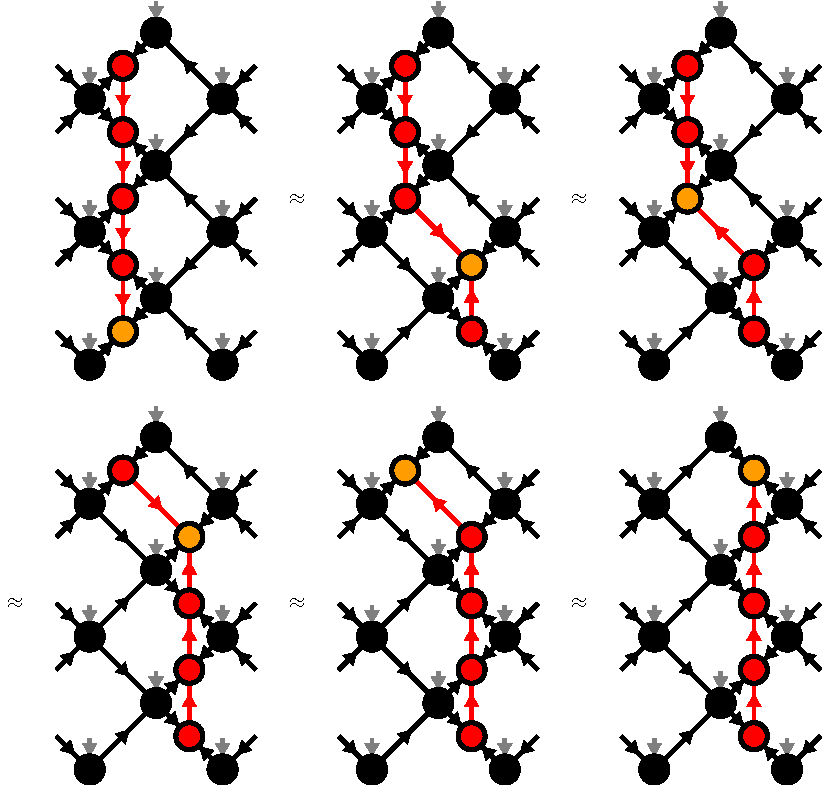
\includegraphics[scale=1]{figures/tikz/disoTPS/shifting_ortho_surface/shifting_ortho_surface.pdf}
	\caption{Two YB-moves are used to shift the orthogonality hypersurface one column to the right. In the last step, the orthogonality center can be moved across the $T$-tensor by contracting the two tensors and performing a truncated SVD.}
	\label{fig:disoTPS_moving_ortho_surface}
\end{figure}
Most algorithms implemented on disoTPS require an efficient procedure for moving the orthogonality surface, where the error introduced by this procedure should be as small as possible. For isoTPS, the current best procedure is given by the Moses Move, followed by an optional variational optimization. \par
In analogy to the MM we look for a procedure to iteratively shift the orthogonality surface through one column of $T$-tensors as shown in figure \figref{fig:disoTPS_moving_ortho_surface}. A single iteration of this process is shown in figure \figref{fig:disoTPS_YB_move_closeup}. The two tensors $W_1$ and $W_2$, which are part of the orthogonality hypersurface, are "pulled through" the site tensor $T$, resulting in the updated tensors $T^\prime$, $W_1^\prime$ and $W_2^\prime$. To keep the isometric structure of the network, $T^\prime$ and $W_1^\prime$ must be isometries, while $W_2^\prime$ must be a tensor of norm one (the new orthogonality center). Due to the visual similarity to the Yang-Baxter equation we call this procedure the \textit{Yang-Baxter} (YB) move. \par
We denote the state represented by the disoTPS before the YB move by $\left|\Psi\right\rangle = \left|\Psi\left(W_1, W_2, T\right)\right\rangle$ and the state after the YB move by $\left|\Psi^\prime\right\rangle = \left|\Psi^\prime\left(W_1^\prime, W_2^\prime, T^\prime\right)\right\rangle$. One can think of the YB move as an optimization problem
\begin{equation}
	\label{eq:disoTPS_YB_move_standard}
	\left(T^\prime_\text{opt},W_{1,\text{opt}}^\prime,W_{2,\text{opt}}^\prime\right) = \underset{T^\prime,W_1^\prime,W_2^\prime}{\argmin}\left\lVert \left|\Psi\right\rangle - \left|\Psi^\prime\right\rangle\right\rVert_\text{F}
\end{equation}
under the constraints
\begin{equation}
	\label{eq:disoTPS_YB_move_constraints}
	T^{\prime\dagger}T^\prime = \id, \quad W_1^{\prime\dagger}W_1^\prime = \id, \quad \left\lVert W_2^\prime \right\rVert_\text{F} = 1.
\end{equation}
One can rewrite the error of the YB move as
\begin{equation}
	\label{eq:disoTPS_YB_move_rewritten_error}
	\begin{split}
		\left\lVert \left|\Psi\right\rangle - \left|\Psi^\prime\right\rangle \right\rVert_\text{F} =& \sqrt{\left\langle\Psi\middle|\Psi\right\rangle + \left\langle\Psi^\prime\middle|\Psi^\prime\right\rangle - 2\Re\left\langle\Psi\middle|\Psi^\prime\right\rangle} \\
		=& \sqrt{2 - 2\Re\left\langle\Psi\middle|\Psi^\prime\right\rangle},
	\end{split}
\end{equation}
where in the second step we used the fact that the wave function is normalized to one, $\left\langle\Psi\middle|\Psi\right\rangle = \left\langle\Psi^\prime\middle|\Psi^\prime\right\rangle = 1$. It follows that the optimization problem of minimizing the error becomes the problem of maximizing the overlap
\begin{equation}
	\label{eq:disoTPS_YB_move_alternative_formulation}
	\left(T^\prime_\text{opt},W_{1,\text{opt}}^\prime,W_{2,\text{opt}}^\prime\right) = \underset{T^\prime,W_1^\prime,W_2^\prime}{\text{argmax}}\Re\left\langle\Psi\middle|\Psi^\prime\right\rangle
\end{equation}
under the constraints \eqref{eq:disoTPS_YB_move_constraints}. Because the only tensors that are changed by the YB move are $W_1$, $W_2$ and $T$ and the three tensors make up a subregion of the full network with only incoming arrows, we can use the isometry condition and the computation of the overlap $\langle\Psi|\Psi^\prime\rangle$ reduces to a contraction of only six tensors as shown in figure \figref{fig:YB_move_iterate_polar_overlap}.\par
\begin{figure}
	\centering
	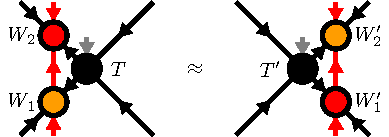
\includegraphics[scale=1]{figures/tikz/disoTPS/yang_baxter_move/yang_baxter_move.pdf}
	\caption{The Yang-Baxter (YB) move is the procedure of "pulling" two auxillary tensors $W_1$ and $W_2$ through a site tensor $T$.}
	\label{fig:disoTPS_YB_move_closeup}
\end{figure}
In the following, we present two explicit algorithms for performing the YB move. The first algorithm (see section \ref{sec:YB_move_iterative_local_optimization}) is an variational optimization method with iterative local updates. The second algorithm (see section \ref{sec:YB_move_svd_disentangle}) is a tripartite decomposition with disentangling similar to the tripartite decomposition used in the MM. In section \ref{sec:YB_move_comparison} we will compare the two algorithms.

\subsection{variational optimization with local updates}
\label{sec:YB_move_iterative_local_optimization}
To solve the constrained optimization problem \eqref{eq:YB_isoTPS_YB_move_alternative_formulation} we proceed by maximizing the overlap while only varying the parameters of one of the three tensors $T^\prime$, $W_1^\prime$ or $W_2^\prime$, treating all other tensors as constant. For example, let us keep $W_1^\prime$ and $W_2^\prime$ fixed and optimize $T^\prime$. We first contract all tensors except $T^\prime$ into an environment $E$ as shown in Figure \figref{fig:YB_move_iterate_polar_optimize_T}. We can then write the optimization problem as
\begin{equation}
	T^\prime_\text{opt} = \underset{T^{\prime\dagger}T = \id}{\argmax} \Re\braket{\Psi,\Psi^\prime} = \underset{T^{\prime\dagger}T = \id}{\argmax}\Re\left\langle E, T^\prime\right\rangle_\text{F} = \underset{T^{\prime\dagger}T = \id}{\argmax}\Re\Tr\left(T^{\prime\dagger}E\right).
\end{equation}
This problem is known as the \textit{orthogonal Procrustes problem} and permits the closed form solution $T^\prime_\text{opt} = UV^\dagger$, where $U$ and $V$ are computed using the SVD $E = USV^\dagger$. For the derivation of this solution see Appendix \ref{app:optimization_problems_for_isometric_tensor_networks}. The tensors $W_1^\prime$ and $W_2^\prime$ can be optimized similarly. The full algorithm is then performed by sweeping over the three tensors, optimizing them iteratively until convergence. Tensor diagrams for the algorithm are shown in Figure \figref{fig:YB_move_iterate_polar}. We discuss one iteration of the algorithm in more detail:
\begin{enumerate}
	\item Contract all tensors except $T^\prime$ into an environment $E$ and perform an SVD $E = USV$. The tensor $T^\prime$ is then updated as $T^\prime\leftarrow UV^\dagger$. See Figure \figref{fig:YB_move_iterate_polar_optimize_T}.
	\item Contract all tensors except $W_1^\prime$ into an environment $E$ and perform an SVD $E = USV$. The tensor $W_1^\prime$ is then updated as $W_1^\prime\leftarrow UV^\dagger$. See Figure \figref{fig:YB_move_iterate_polar_optimize_W1}.
	\item Contract all tensors except $W_2^\prime$ into an environment $E$. The tensor $W_1^\prime$ is then updated as $W_1^\prime\leftarrow E/\left\lVert E\right\rVert$. See Figure \figref{fig:YB_move_iterate_polar_optimize_W2}.
\end{enumerate}
These three steps are repeated until a termination criterion is met, for example until the decrease in error after one iteration is smaller than a given threshold or if a given maximum number of iterations $N_\text{iter}$ is exceeded. A similar algorithm was also used by Evenbly and Vidal in the context of the multi-scale entanglement renormalization ansatz
(MERA) \cite{cite:algorithms_for_entanglement_renormalization, cite:algorithms_for_entanglement_renormalization_boundaries_impurities_interfaces}. Note that in step three of the algorithm, a norm constraint is enforced instead of an isometry constraint, in which case the closed form solution takes a different shape. We also derive this solution in Appendix \ref{app:optimization_problems_for_isometric_tensor_networks}.\par
\begin{figure}
	\centering
	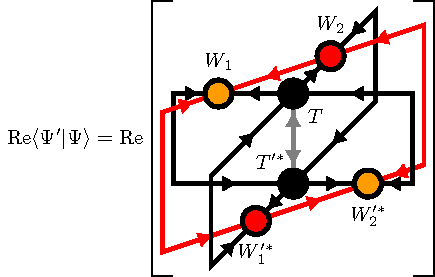
\includegraphics[scale=1]{figures/tikz/YB_isoTPS/yang_baxter_move_iterative/yang_baxter_move_iterative_a.pdf}
	\caption{The cost function of the optimization problem \eqref{eq:YB_isoTPS_YB_move_alternative_formulation} can be computed as a contraction of only six tensors.}
	\label{fig:YB_move_iterate_polar_overlap}
\end{figure}
\begin{figure}
	\centering
	\begin{subfigure}[c]{0.85\textwidth}
		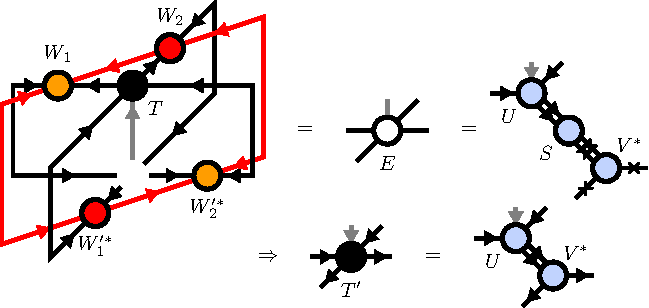
\includegraphics[scale=1]{figures/tikz/YB_isoTPS/yang_baxter_move_iterative/yang_baxter_move_iterative_b.pdf}
		\caption{}\label{fig:YB_move_iterate_polar_optimize_T}
	\end{subfigure}
	\begin{subfigure}[c]{0.85\textwidth}
		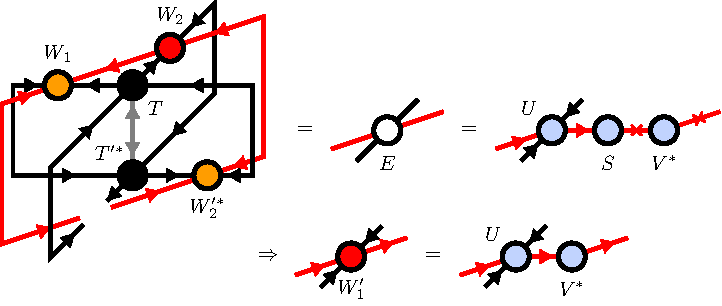
\includegraphics[scale=1]{figures/tikz/YB_isoTPS/yang_baxter_move_iterative/yang_baxter_move_iterative_c.pdf}
		\caption{}\label{fig:YB_move_iterate_polar_optimize_W1}
	\end{subfigure}
	\begin{subfigure}[c]{0.85\textwidth}
		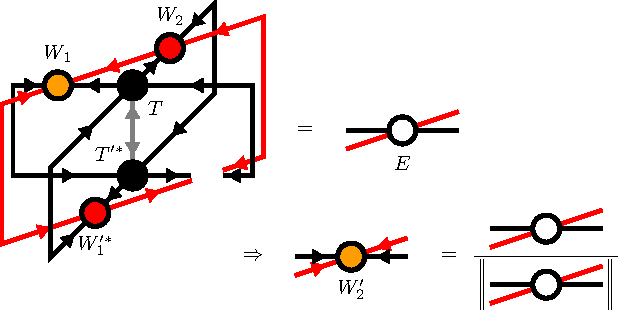
\includegraphics[scale=1]{figures/tikz/YB_isoTPS/yang_baxter_move_iterative/yang_baxter_move_iterative_d.pdf}
		\caption{}\label{fig:YB_move_iterate_polar_optimize_W2}
	\end{subfigure}%
	\caption{In this figure we show the three local updates that are used to iteratively solve optimization problem \eqref{eq:YB_isoTPS_YB_move_alternative_formulation}. (a) The tensor $T^\prime$ can be updated similarly by contracting all tensors except $T^\prime$ into the environment $E$ and isometrizing $E$ using an SVD. (b) The tensor $W_1^\prime$ can be updated by contracting all tensors except $W_1^\prime$ into the environment $E$, which is subsequently isometrized using an SVD. (c) To optimize the tensor $W_2^\prime$, all tensors except $W_2^\prime$ are contracted into the environment $E$. The updated tensor is then given as $W_2^\prime = E/\lVert E\rVert$.}
	\label{fig:YB_move_iterate_polar}
\end{figure}
The computational cost of the algorithm is dominated by the tensor contractions, scaling as $\mathcal{O}(3N_\text{iter}(\chi^2D^6d + \chi^3D^4)) = \mathcal{O}(N_\text{iter}D^8)$ for one YB move.\par
\input{figures/plots/YB_isoTPS/yb_move_iterate_polar.tex}
In practice we observe that the discussed algorithm converges only very slowly. To qualitatively showcase this, we perform the YB move on a typical environment of tensors $\left\{W_1, W_2, T\right\}$ that was encountered during imaginary time evolution of the Transverse Field Ising model, see Chapter \ref{chap:TFI} for more details. The bond dimensions chosen for the YB-isoTPS are $D = 4$, $\chi = 24$. We plot the error $\lVert\ket{\Psi}-\ket{\Psi^\prime}\rVert$ against the number of iterations in Figure \figref{fig:YB_isoTPS_tripartite_decomposition_iterate_polar}. After $N_\text{iter}=10000$ iterations, the algorithm is still not converged.

\subsection{Tripartite decompositon using an SVD and disentangling}
\label{sec:YB_move_svd_disentangle}
Alternatively, the constrained optimization problem \eqref{eq:disoTPS_YB_move_standard} can be solved via two successive SVDs with an optional disentangling prodcedure with the goal of reducing the truncation error or some entanglement measure. This is the same algorithm that was used for the MM in the original isoTPS \cite{cite:efficient_simulation_of_dynamics_in_two_dimensional_quantum_spin_systems}. The algorithm is sketched in figure \figref{} and is made up of three main steps.
\begin{enumerate}
	\item We start by contracting the tensors $T$, $W_1$ and $W_2$ into a single tensor $\Psi$ (figure \figref{} (b)). This tensor is then split from left to right via a truncated SVD
	\begin{equation}
		\Psi = XSZ^\dagger = X\left(SZ^\dagger\right) \eqqcolon X\theta
	\end{equation}
	as shown in figure \figref{}(c). The bond dimension is truncated to $D^2$.
	\item Next, we split the index of the bond connecting $X$ and $\theta$ into two indices of dimension $D$ each, see figure \figref{}(d). To proceed, we note that there exists a degree of freedom on the bonds connecting $X$ and $\theta$: A unitary $U$ and its adjoint can be inserted as shwon in figure \figref{}(e) without changing the result of the contraction
	\begin{equation}
		XU^\dagger U\theta = \left(XU^\dagger\right)\left(U\theta\right) \eqqcolon T^\prime \tilde{\theta}.
	\end{equation}
	This unitary $U$ can be chosen to minimize the truncation error of the next step by \textit{disentangling} the tensor $\theta$. We will discuss procedures of finding such a \textit{disentangling unitary} on the next page.
	\item In the last step, the tensor $\tilde{\theta}$ is split vertically into $W_1^\prime$ and $W_2^\prime$ using a truncated SVD as shown in figure \figref{}(f). Here, the bond dimension is truncated to $\chi$. We end up with the three tensors $T^\prime$, $W_1^\prime$ and $W_2^\prime$, completing the YB move.
\end{enumerate}
Before we discuss the disentangling procedure, two comments about step two of the above algorithm are in order. Firstly, there exists a degree of freedom for splitting the bond index, because applying the same permutations to the columns of $X$ and rows of $\theta$ does not change the result of contracting the network. Thus, there is no unique splitting that can be chosen. However, this degree of freedom is fixed by the disentangling process, making the exact permutation of the bond splitting irrelevant. Secondly, note that near the edges of the lattice it can happen that the matrizized tensor $\Psi$ has $\tilde{\chi} < D^2$ rows. In this case, the bond dimension after the SVD will also be $\tilde{\chi}$ and we cannot split the bond into two bonds of dimension $\chi_1=\chi_2=D$. Instead, we choose a splitting $\chi_1 \le D$, $\chi_2 \le D$ such that $\chi_1\cdot\chi_2$ is maximized while it must still hold $\chi_1\cdot\chi_2\le\tilde{\chi}$. We additionally prefer "equal" splittings $\chi_1\approx\chi_2\approx\sqrt{\tilde{\chi}}$ if possible. One can find such a splitting easily by computing all possible combinations of $\chi_1$ and $\chi_2$ and keeping only the best one. This has a computational cost of $\mathcal{O}\left(\sqrt{\tilde{\chi}}\right) = \mathcal{O}\left(d\right)$. \par
\begin{figure}
	%\includegraphics[width=0.8\textwidth]{figures/Tensor_Networks/yb_move_svd_disent.jpeg}
	\caption{test\todo{Why does this image not work? Also write caption.}}
	\label{fig:yb_move_svd_disent}
\end{figure}
We will now discuss the problem of finding a good disentangling unitary $U$ for step two of the above algorithm, which is crucial for the performance of the YB move. The problem can be formulated as follows: Given a tensor $\theta \in \mathbb{C}^{\chi_1\times d_1\times d_2\times \chi_2}$, find a unitary $U\in\mathbb{C}^{d_1\times d_2\times d_1\times d_2}$ minimizing a cost function
\begin{equation}
	f(\tilde{\theta}),
\end{equation}
where
\begin{equation}
	\tilde{\theta}\in\mathbb{C}^{\chi_1\times d_1\times d_2\times \chi_2}, \quad \tilde{\theta}_{\alpha,i,j,\beta} \coloneqq \sum_{i^\prime,j^\prime}U_{i,j,i^\prime,j^\prime}\theta_{\alpha,i,j,\beta}.
\end{equation}

\subsection{Comparison of the two algorithms}
\label{sec:YB_move_comparison}
\input{figures/plots/disoTPS/yb_move_comparison.tex}

\section{Time Evolving Block Decimation (TEBD)}
\label{sec:disoTPS_TEBD}
We will now discuss the Time Evolving Block Decimation (TEBD) algorithm for disoTPS, which can be used for both real and imaginary time evolution. The algorithm is a generalization of TEBD for MPS, which we discussed in Section \ref{sec:tensors_and_tensor_networks_matrix_product_states}. Analogously to MPS we start with a Suzuki-Trotter decomposition, approximating the time evolution operator $U\left(\Delta t\right) = e^{-i\Delta t \hat{H}}$ by a product of bond operators $U^{[x, y]}\left(\Delta t\right)$ acting only on neighbouring sites on the bond $[x, y]$. These bond operators then must be applied to the state in the correct order, while keeping the disoTPS structure intact. We will discuss the process of applying a single bond operator $U^{[x,y]}\left(\Delta t\right)$ to the disoTPS in Section \ref{sec:YB_isoTPS_TEBD_local_updates}. In Section \ref{sec:YB_isoTPS_TEBD_global_updates} we then discuss the full TEBD algorithm.

\subsection{Local TEBD updates}
\label{sec:YB_isoTPS_TEBD_local_updates}
\begin{figure}
	\centering
	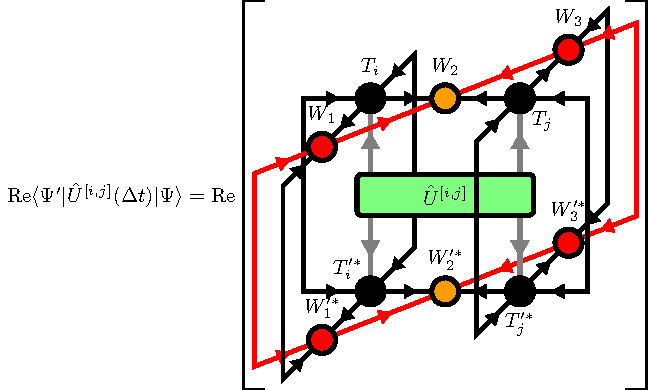
\includegraphics[scale=1]{figures/tikz/YB_isoTPS/tebd_environment/tebd_environment.pdf}
	\caption{The cost function of the optimization problem \eqref{eq:YB_isoTPS_TEBD_maximizing_overlap} that must be solved for locally applying TEBD operators $\hat{U}^{[i,j]} \coloneqq \hat{U}^{[i,j]}(\Delta t)$ can be computed as a contraction of the two-site wave functions of $\ket{\Psi}$ and $\ket{\Psi^\prime}$, sandwiching the operator between the two.}
	\label{fig:YB_isoTPS_TEBD_overlap_contraction}
\end{figure}
Let us assume that the orthogonality center is positioned between the two sites on which the bond operator $\hat{U}^{[x, y]}\left(\Delta t\right)$ acts. The five tensors around the orthogonality center then make up a sub-network with only incoming arrows, compare Figure \figref{fig:YB_isoTPS_twosite_expectation_value_environment}. We call these five tensors $T_1$, $T_2$, $W_1$, $W_2$ and $W_3$. The local TEBD update can then be formulated as the following problem: Find tensors $T_1^\prime$, $T_2^\prime$, $W_1^\prime$, $W_2^\prime$ and $W_3^\prime$ satisfying the isometry constraints and minimizing the error
\begin{equation}
	\label{eq:isoDTPS_TEBD_local_update_error}
	\varepsilon_\text{trunc} = \left\lVert \hat{U}^{[x,y]}(\Delta t)\ket{\Psi} - \ket{\Psi}\right\rVert
\end{equation}
Similar to the YB-move, we can rewrite this as the problem of maximizing the overlap
\begin{equation}
	\label{eq:YB_isoTPS_TEBD_maximizing_overlap}
	(T_{i,\text{opt}}^\prime, T_{j,\text{opt}}^\prime, W_{1,\text{opt}}^\prime, W_{2,\text{opt}}^\prime, W_{3,\text{opt}}^\prime)= \underset{T_i^\prime, T_j^\prime, W_1^\prime, W_2^\prime, W_3^\prime}{\argmax}\Re\bra{\Psi}\hat{U}^{[x,y]}(\Delta t)\ket{\Psi^\prime}.
\end{equation}
under the constraints $T_i^{\prime\dagger}T_i^\prime = \id$, $T_j^{\prime\dagger}T_j^\prime = \id$, $W_1^{\prime\dagger}W_1^\prime = \id$, $W_3^{\prime\dagger}T_3^\prime = \id$ and $\lVert W_2^\prime\rVert = 1$.
Using the isometry condition, the overlap $\bra{\Psi}\hat{U}^{[x,y]}(\Delta t)\ket{\Psi^\prime}$ can be computed by contracting the tensor network drawn in Figure \figref{fig:YB_isoTPS_TEBD_overlap_contraction}. For solving this problem we again use the Evenbly-Vidal algorithm. Similar to what we already did in Section \ref{sec:YB_move_iterative_local_optimization} for the YB move, we optimize one tensor at a time while keeping all other tensors fixed. This procedure is then repeated, sweeping over all five tensors until convergence is achieved. For more details on this optimization method see Appendix \ref{app:riemannian_optimization_of_isometries}. Since the time step $\Delta t$ is chosen to be small, the bond operator is close to identity, $\hat{U}^{[x,y]}(\Delta t)\approx\id$. Thus, a good initialization for the tensors of the updated wave function $\ket{\Psi^\prime}$ are simply the tensors of the old wave function $\ket{\Psi}$. \par
The computational complexity of applying a local bond operator to a disoTPS with the discussed algorithm scales as $\mathcal{O}(\chi^3D^3d^2) = \mathcal{O}(D^6)$. In practice it is observed that the algorithm converges after only a few iterations.

\subsection{Global TEBD updates}
\label{sec:YB_isoTPS_TEBD_global_updates}
\begin{figure}
	\centering
	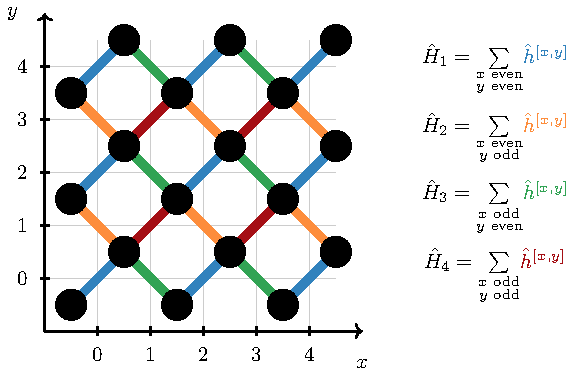
\includegraphics[scale=1]{figures/tikz/YB_isoTPS/tebd_global_update/tebd_global_update_a.pdf}
	\caption{A Hamiltonian $\hat{H}$ that is a sum of nearest-neighbour operators $h^{[x,y]}$ can be split into four parts made up of operators acting only on even/odd columns and even/odd bonds along a column.}
	\label{fig:YB_isoTPS_TEBD_global_update_TEBD1_splitting_and_TEBD2_chain}
\end{figure}
A global TEBD update evolves the state by a time $\Delta t$ and can be performed by applying local TEBD updates on all bonds. For each local TEBD update, the orthogonality center must be moved to the bond at which the update is applied. Because moving the orthogonality hypersurface can only be done approximately, the number of necessary moves should be minimized. \par
As we have already done for MPS in Section \ref{sec:tensors_and_tensor_networks_matrix_product_states}, let us assume that the Hamiltonian $\hat{H}$ can be written as a sum of nearest-neighbour operators. We index these nearest-neighbour operators $h^{[x, y]}$ by two integers $x$ and $y$ corresponding to the position of the orthogonality hypersurface and orthogonality center if moved to the bond on which $h^{[x,y]}$ acts. We define $x$ to increase from left to right and $y$ to increase from bottom to top, as shown in Figure \figref{fig:YB_isoTPS_TEBD_global_update_TEBD1_splitting_and_TEBD2_chain}. The Hamiltonian can then be split into four parts by first grouping the $h^{[x,y]}$ into two sets acting only on even and odd columns respectively and then splitting each set again into terms acting only on even/odd bonds along the respective columns. We can write this as
\begin{equation}
	\label{eq:YB_isoTPS_TEBD_splitting_local_Hamiltonian}
	\begin{split}
		\hat{H} = \sum_{x=1}^{2L_x-1} \sum_{y=1}^{2L_y-1}h^{[x,y]} &= \sum_{\substack{x\text{ even}\\y\text{ even}}} h^{[x, y]} + \sum_{\substack{x\text{ even}\\y\text{ odd}}} h^{[x, y]} + \sum_{\substack{x\text{ odd}\\y\text{ even}}} h^{[x, y]} + \sum_{\substack{x\text{ odd}\\y\text{ odd}}} h^{[x, y]} \\
		&\eqqcolon \hat{H}_1 + \hat{H}_2 + \hat{H}_3 + \hat{H}_4.
	\end{split}
\end{equation}
The operators appearing in the sum in $\hat{H}_j$ commute with each other and thus the exponential $e^{-i\Delta t\hat{H}_j}$ factorizes into a product of bond operators $\hat{U}^{[x, y]}(\Delta t) = e^{-i\Delta t\hat{h}^{[x, y]}}$. \par
We next use a Suzuki-Trotter decomposition to approximate the time evolution operator
\begin{equation}
	\label{eq:YB_isoTPS_TEBD_suzuki_trotter_first_order}
	\hat{U}(\Delta t) = \hat{U}^\text{TEBD1}(\Delta t) + \mathcal{O}(\Delta t^2)
\end{equation}
with
\begin{equation}
	\label{eq:YB_isoTPS_TEBD_first_order_TEBD_operator}
	\hat{U}^\text{TEBD}(\Delta t) \coloneqq e^{-i\Delta t\hat{H}_4} e^{-i\Delta t\hat{H}_3} e^{-i\Delta t\hat{H}_2} e^{-i\Delta t\hat{H}_1}.
\end{equation}
To evolve the state $\ket{\Psi}$ in time with this first order approximation we must compute $\ket{\Psi^\prime} \approx U^\text{TEBD1}(\Delta t)\ket{\Psi}$ as a disoTPS. The procedure is sketched in Figure \figref{fig:YB_isoTPS_TEBD_global_update_applying_TEBD1}. We start in the left-most column and apply all bond operators that act on bonds along this column. The bond operators on the column are applied in a brick-wall fashion analogously to the MPS algorithm: First all even bonds are updated and then all odd bonds are updated. Local updates are computed using the algorithm discussed in Section \ref{sec:YB_isoTPS_TEBD_local_updates}. Next, we move the orthogonality hypersurface two columns to the right and again apply all bond operators along the column. We proceed until all bond operators on even columns have been applied, in which case the orthogonality hypersurface is now positioned at its right-most position. We now sweep back to the left, applying all bond operators acting on odd columns along the way. Arriving back at the left-most column, all bonds making up $\hat{U}^\text{TEBD1}(\Delta t)$ have been applied in the correct order and the state has been evolved by time $\Delta t$. \par
\begin{figure}
	\centering
	\subcaptionbox{\label{fig:YB_isoTPS_TEBD_global_update_applying_TEBD1}}
	{%
		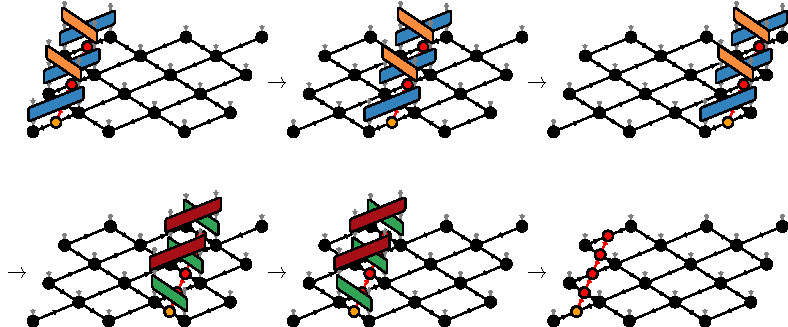
\includegraphics[scale=1]{figures/tikz/YB_isoTPS/tebd_global_update_steps/tebd_global_update_steps_a.pdf}
	}
	\par\bigskip\medskip
	\subcaptionbox{\label{fig:YB_isoTPS_TEBD_global_update_applying_TEBD2}}
	{%
		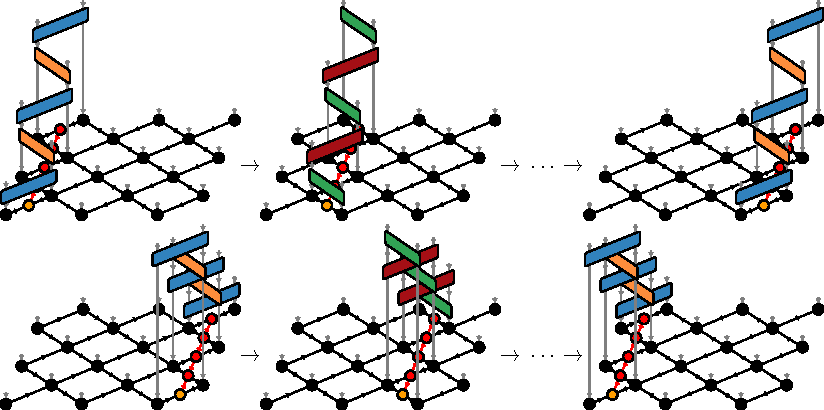
\includegraphics[scale=1]{figures/tikz/YB_isoTPS/tebd_global_update_steps/tebd_global_update_steps_b.pdf}
	}
	\caption{To apply a TEBD update, we sweep across the disoTPS once from left to right and back from right to left. (a) TEBD1 applies the operators in a brick-wall fashion, while (b) TEBD2 applies the operators along a chain.}
	\label{fig:YB_isoTPS_TEBD_global_update_applying_TEBD}
\end{figure}
We can obtain a better approximation of the time evolution operator $U(\Delta t)$ by performing a second order Suzuki-Trotter decomposition. By repeatedly applying the symmetrized decomposition
\begin{equation}
	e^{-i\varepsilon(A+B)} = e^{-i\frac{\varepsilon}{2}A}e^{-i\frac{\varepsilon}{2}A}e^{-i\varepsilon B} + \mathcal{O}(\Delta t^3)
\end{equation}
we obtain
\begin{equation}
	\begin{split}
		\label{eq:YB_isoTPS_tebd_second_order_suzuki_trotter_decomposition}
		e^{-i\Delta t\hat{H}} &= \exp\left(-i\Delta t\sum_{x,y}\hat{h}^{[x,y]}\right) \\
		&= e^{-i\frac{\Delta t}{2}\hat{h}^{[1, 1]}} e^{-i\Delta t\left(\hat{H}-\hat{h}^{[1,1]}\right)} e^{-i\frac{\Delta t}{2}\hat{h}^{[1, 1]}} + \mathcal{O}(\Delta t^3)\\
		&= e^{-i\frac{\Delta t}{2}\hat{h}^{[1, 1]}} e^{-i\frac{\Delta t}{2}\hat{h}^{[1, 2]}} e^{-i\Delta t\left(\hat{H}-\hat{h}^{[1,1]}-\hat{h}^{[1, 2]}\right)} e^{-i\frac{\Delta t}{2}\hat{h}^{[1, 2]}} e^{-i\frac{\Delta t}{2}\hat{h}^{[1, 1]}} + \mathcal{O}(\Delta t^3)\\
		&=\cdots\\
		&= e^{-i\frac{\Delta t}{2}\hat{h}^{[1, 1]}} e^{-i\frac{\Delta t}{2}\hat{h}^{[1, 2]}} \cdots e^{-i\frac{\Delta t}{2}\hat{h}^{[1, 2]}} e^{-i\frac{\Delta t}{2}\hat{h}^{[1, 1]}} + \mathcal{O}(\Delta t^3).
	\end{split}
\end{equation}
Here, in each step we "split off" one operator $\hat{h}^{[x,y]}$ from the sum. The final result is a product of bond operators $\hat{U}^{[x,y]}(\Delta t/2))$ that must be applied from right to left. The algorithm of applying a global second order update is thus similar to a TEBD update of first order. We sweep across the disoTPS once from left to right and back, applying bond operators along the way in the correct order, as visualized in Figure \figref{fig:YB_isoTPS_TEBD_global_update_applying_TEBD2}. The difference to TEBD1 is that now the operators are applied in a chain-like order instead of the brick wall order of TEBD1. The number of YB moves for TEBD1 and TEBD2 is the same, but the smaller Trotter error of $\mathcal{O}(\Delta t^3)$ instead of $\mathcal{O}(\Delta t^2)$ allows us to use larger time steps for TEBD2, resulting in a smaller number of YB moves per unit time. We find that the YB move is the primary source of error in practice and thus expect TEBD2 to perform much better than TEBD1. \par 
In principle, one could also go to higher decomposition orders \cite{cite:finding_exponential_product_formulas_of_higher_orders}. However, already a third order decomposition would necessitate a larger number of sweeps for applying the full update, increasing the error accumulated through YB moves. It is therefore not clear if higher order decompositions would be able to improve the method further.

	
	\chapter{Toric Code: An exactly representable Model}
	In this chapter we show that the YB-isoTPS ansatz introduced in Chapter \ref{chap:isoTPS_alternative_canonical_form} is able to exactly represent the ground state of the Toric Code Model. We first give a brief introduction to the Toric Code model in Section \ref{sec:the_toric_code_model} and show how the ground state can be derived analytically. We then discuss how this ground state can be represented as a YB-isoTPS in Section \ref{sec:representing_the_toric_code_gs_with_YB_isoTPS}.

\section{The Toric Code Model}
\label{sec:the_toric_code_model}
The Toric Code is an exactly soluble spin model with $\mathbb{Z}_2$ topological order that was introduced by Alexei Kitaev \cite{cite:fault_tolerant_quantum_computation_by_anyons}. The model is defined on the square lattice with periodic boundary conditions, where on each edge of the lattice there sits a spin-1/2 degree of freedom. Two operators are introduced, the \textit{star operators}
\begin{equation}
	\label{eq:star_operator}
	\hat{A}_+ \coloneqq \sum_{j\in+}\hat{\sigma}_j^z
\end{equation}
and the \textit{plaquette operators}
\begin{equation}
	\label{eq:plaquette_operator}
	\hat{B}_{\scalebox{0.6}{$\square$}} \coloneqq \sum_{j\in \scalebox{0.6}{$\square$}} \hat{\sigma}_j^x,
\end{equation}
where the sums are performed over the four spins connected in a star or plaquette pattern respectively (see Figure \figref{fig:toric_code_star_and_plaquette_operators}) and $\hat{\sigma}_j^x, \hat{\sigma}_j^z$ are Pauli matrices. The Hamiltonian of the Toric Code model is then defined as
\begin{equation}
	\label{eq:toric_code_hamiltonian}
	H_\text{TC} \coloneqq -\sum_+\hat{A}_+ - \sum_{\scalebox{0.6}{$\square$}}\hat{B}_{\scalebox{0.6}{$\square$}},
\end{equation}
where the sums go over all possible stars and plaquettes respectively. Because an arbitrary star and plaquette operator share either two or zero spins, all terms of the Hamiltonian commute and it is thus possible to find the ground state of the model by diagonalizing all terms simultaneously. To diagonalize the star operators $\hat{A}_+$ we choose a basis of $\hat{\sigma}_z$-eigenstates $\ket{i} \in \left\{\ket{\uparrow}, \ket{\downarrow}\right\}$ with eigenvalues $\left\langle\hat{\sigma}_z\right\rangle_i = s_i = \pm 1$ for each spin $i$. In this basis every star operator is diagonal with eigenvalues
\begin{equation}
	\label{eq:toric_code_star_operator_expectation value}
	\langle \hat{A}_+\rangle = \prod_{j\in+}s_j \in \left\{1, -1\right\}.
\end{equation}
To obtain the expectation value $\langle \hat{A}_+\rangle = 1$, the number of spins in the down state $s_j = -1$ around the vertex $+$ must be even. Basis states $\ket{s}$ that give an expectation value of $1$ for every star operator simultaneously are thus the states with an even number of down-spins around every vertex,
\begin{equation}
	\label{eq:toric_code_A_operator_condition}
	\ket{s} = \ket{s_1} \otimes \dots \otimes \ket{s_N}, \quad \prod_{j\in+}s_j = 1 \,\,\,\,\forall +.
\end{equation}
The plaquette operator $\hat{B}_{\scalebox{0.6}{$\square$}}$ acts on a basis state by flipping all spins around the plaquette $\scalebox{0.6}{$\square$}$. Because a plaquette and a star share either zero or two spins, applying an plaquette operator to a state $\ket{s}$ satisfying condition \eqref{eq:toric_code_A_operator_condition} produces a state $\ket{s^\prime}$ that again satisfies \eqref{eq:toric_code_A_operator_condition}, and applying the plaquette operator a second time produces the initial state $\ket{s}$. If we now take the equal weighted superposition $\ket{\Psi} = \left(\ket{s}+\ket{s^\prime}\right)/\sqrt{2}$, the expectation value of $\hat{B}_{\scalebox{0.6}{$\square$}}$ becomes $\langle \hat{B}_{\scalebox{0.6}{$\square$}}\rangle = 1$.
The ground state of the Hamiltonian \eqref{eq:toric_code_hamiltonian} is thus given by the equal weighted superposition of all basis states satisfying condition \eqref{eq:toric_code_A_operator_condition}. \par
One can show that the ground state can be written as
\begin{equation}
	\ket{\Psi_0} \propto \prod_{\scalebox{0.6}{$\square$}}\left(\id + \hat{B}_{\scalebox{0.6}{$\square$}}\right) \ket{\uparrow} \otimes \dots \otimes \ket{\uparrow}.
\end{equation}
Note that this is also the ground state for the model if open boundary conditions are chosen instead. \par
For periodic boundary conditions, which is equivalent to putting the model on a torus, one can further show that the ground state is fourfold topologically degenerate. To move from one degenerate section of the Hilbert space to another one must apply a string of operators, wrapping once around the torus. This is a highly non-local operation. Because perturbations are usually local, the toric code model can be interpreted as a form of hardware level error correction. The toric code is considered a topological quantum error correction code and can in theory be used for quantum memory. One can further implement quantum gates acting on the 4-dimensional ground state space by locally creating a pair of anyonic excitations, moving one of the excitations around the torus, and annihilating it with the other one \cite{cite:fault_tolerant_quantum_computation_by_anyons}. Unfortunately, the gates that can be implemented as such do not form a complete state set and thus do not allow for universal quantum computing. Nevertheless, the Toric code is an important model for the study of topological order and anyonic excitations.
\begin{figure}
	\centering
	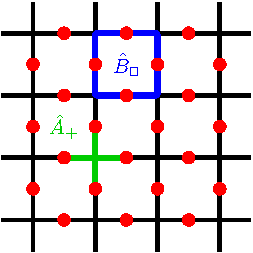
\includegraphics[scale=1]{figures/tikz/toric_code/toric_code_general/toric_code_general.pdf}
	\caption{The Toric Code model is defined on the square lattice with spin-1/2 degrees of freedom living on the edges. the star and plaquette operators \eqref{eq:star_operator} and \eqref{eq:plaquette_operator} act on the four spins arranged in a star or plaquette shape respectively.}
	\label{fig:toric_code_star_and_plaquette_operators}
\end{figure}


\section{Representing the Toric Code Ground State with YB-isoTPS}
\label{sec:representing_the_toric_code_gs_with_YB_isoTPS}
\begin{figure}
	\centering
	\subcaptionbox{\label{fig:toric_code_doubling_dof}}
	{%
		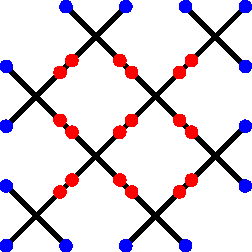
\includegraphics[scale=1]{figures/tikz/toric_code/peps_representation/peps_representation_a.pdf}
	}
	\quad
	\subcaptionbox{\label{fig:toric_code_PEPS_representation_tensor_definitions}}
	{%
		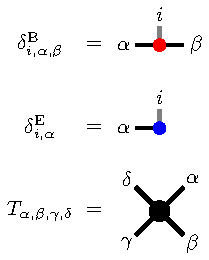
\includegraphics[scale=1]{figures/tikz/toric_code/peps_representation/peps_representation_b.pdf}
	}
	\quad
	\subcaptionbox{\label{fig:toric_code_PEPS_representation}}
	{%
		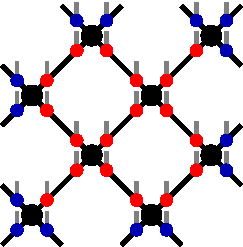
\includegraphics[scale=1]{figures/tikz/toric_code/peps_representation/peps_representation_c.pdf}
	}
	\caption{(a) To represent the Toric Code ground state as a PEPS we start by doubling the local degrees of freedom on each edge in the bulk. Bulk spins are denoted in red, while boundary spins are coloured blue. (b) Tensor diagrams of the tensors $\delta^\text{B}$, $\delta^\text{E}$ and $T$ introduced in the text. (b) The PEPS representation of the Toric Code ground state before contracting the tensors at each vertex, made up from the tensors (b).}
	\label{fig:toric_code_doubling_dof_and_PEPS_representation}
\end{figure}
\begin{figure}
	\centering
	\savebox{\largestimage}{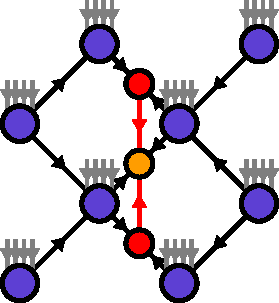
\includegraphics[scale=1]{figures/tikz/toric_code/YB_isoTPS_representation/YB_isoTPS_representation_a.pdf}}
	\subcaptionbox{\label{fig:toric_code_YB_isoTPS_representation}}
	{%
		\usebox{\largestimage}
	}
	\quad\quad\quad
	\subcaptionbox{\label{fig:toric_code_YB_isoTPS_representation_tensor_definitions}}
	{%
		\raisebox{\dimexpr.5\ht\largestimage-.5\height}
		{%
			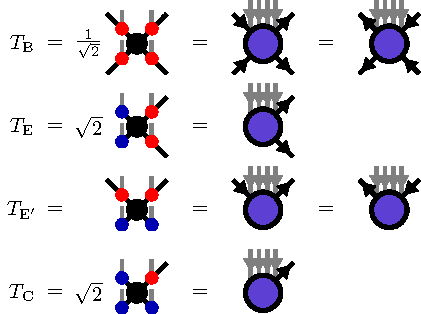
\includegraphics[scale=1]{figures/tikz/toric_code/YB_isoTPS_representation/YB_isoTPS_representation_b.pdf}
		}
	}
	\caption{The PEPS in figure \protect\figref{fig:toric_code_PEPS_representation} can be transformed to the disoTPS (a) by normalizing the tensors as shown in (b). Note that the tensors $T_\text{E}^\prime$ at the top and bottom edges of the lattice need a different normalization than the tensors $T_\text{E}$ at the left and right edges.}
	\label{fig:toric_code_YB_isoTPS}
\end{figure}
We will now derive the disoTPS corresponding to the Toric Code ground state on a square lattice with open boundary condition. We choose rough boundary conditions \cite{cite:models_for_gapped_boundaries_and_domain_walls}, fixing all boundary spins to the state $\left(\ket{\uparrow} + \ket{\downarrow}\right)/\sqrt{2}$. As shown in \cite{cite:isometric_tensor_network_representation_of_string_net_liquids}, the Toric Code ground state can be represented exactly as a PEPS with bond dimension $D = 2$. One can construct such a PEPS easily by first doubling the Hilbert space on each edge as $\ket{s_i} \rightarrow \ket{s_i}\otimes\ket{s_i}$, which we show in Figure \figref{fig:toric_code_doubling_dof}. In the PEPS representation the physical degrees of freedom on each edge in the bulk are then carried by two identical tensors $\delta^\text{B}\in\mathbb{R}^{2\times2\times2}$,
\begin{equation}
	\delta^\text{B}{i,\alpha,\beta} = \begin{cases}
		1 &\text{if }i=\alpha=\beta\\
		0 &\text{else}
	\end{cases},
\end{equation}
as shown in Figure \figref{fig:toric_code_PEPS_representation_tensor_definitions}. The boundary spins are represented by tensors $\delta_E\in\mathbb{R}^{2\times2}$,
\begin{equation}
	\delta^\text{E}{i,\alpha} = \begin{cases}
		1 &\text{if }i=\alpha\\
		0 &\text{else}
	\end{cases}.
\end{equation}
We proceed by associating each vertex with the spins on the four connected edges and connect the corresponding tensors $\delta^\text{B}$ and $\delta^\text{E}$ with a tensor $T\in\mathbb{R}^{2\times2\times2\times2}$ that is placed on each vertex,
\begin{equation}
	T_{i,j,k,l} = \begin{cases}
		1 & \text{if } \left(i+j+k+l\right)\mod2 = 0 \\
		0 & \text{else}
	\end{cases}.
\end{equation}
This tensor ensures that all states with an odd number of down spins around a vertex have an amplitude of zero, satisfying condition \eqref{eq:toric_code_A_operator_condition}. \par
We arrive at the PEPS in Figure \figref{fig:toric_code_PEPS_representation}. Each basis state satisfying condition \eqref{eq:toric_code_A_operator_condition} results in the same amplitude when contracting the PEPS, while basis states violating the condition vanish. Thus, the PEPS represents the ground state of the Toric Code. \par
We now want to transform the PEPS into a disoTPS. This can be easily done by choosing the correct normalization for the vertex tensors, which transforms them into isometries as shown in Figure \figref{fig:toric_code_YB_isoTPS_representation_tensor_definitions}. Note that different normalizations need to be chosen for tensors at the corners, edges, and in the bulk. For each vertex tensor we can choose the isometry direction to point to the left or to the right respectively, allowing us to place the orthogonality hypersurface anywhere in the lattice. As a last step, the tensors of the orthogonality hypersurface must be specified. The two spins that are connected to a tensor $W$ of the orthogonality hypersurface must be in the same local state, since they were created by doubling the local degree of freedom. This constraint can be enforced by setting $W\in\mathbb{R}^{2\times1\times2\times1}$ to
\begin{equation}
	W_{\alpha,\nu,\beta,\mu} = \frac{\delta_{\alpha,\beta}}{\sqrt{2}}
\end{equation} 
with dummy indices $\nu, \mu$ of bond dimension $1$. Trivially, the tensors $W$ fulfil the isometry condition. We can again choose the direction of isometry to point either up or down for every $W$-tensor, allowing us to place the orthogonality center freely along the orthogonality hypersurface.\par
We have thus found an exact disoTPS representation of the Toric Code ground state with $D = 2$ and $\chi= 1$, similar to the construction done in \cite{cite:isometric_tensor_network_representation_of_string_net_liquids} for isoTPS. The final network is depicted in Figure \figref{fig:toric_code_YB_isoTPS_representation}. We test the different algorithms for the YB move on the Toric Code ground state on a $5\times5$ lattice. All algorithms are able to move the orthogonality surface exactly up to computational accuracy. This however only works well if a good initialization is chosen for the disentangling unitary. We choose an initialization based on an SVD, see \cite{cite:isometric_tensor_network_states_in_two_dimensions, cite:efficient_simulation_of_dynamics_in_two_dimensional_quantum_spin_systems} or our implementation \cite{cite:github_YB_isoTPS}.
	
	\chapter{Transverse Field Ising Model: Ground State Search and Time Evolution}
	The Transverse Field Ising (TFI) Model is a well-studied spin lattice model that is often used to benchmark numerical methods. We introduce the TFI model in Section \ref{sec:TFI_model}. We then proceed by benchmarking YB-isoTPS methods on the model. We first perform ground state searches using imaginary time evolution in Section \ref{sec:TFI_ground_state_search}. We benchmark the different proposed algorithms for the YB move and compare the first and second order TEBD algorithms. We further show numerical evidence that YB-isoTPS are able to capture area law entanglement. Lastly we perform a ground state search on the honeycomb lattice, showing that YB-isoTPS can be easily generalized to different lattice types. In Section \ref{sec:TFI_time_evolution} we perform a global quench and compute real time evolution. We observe that YB-isoTPS struggles with the rapid entanglement growth and discuss some ideas for overcoming the problem. \par
We compare the results obtained with YB-isoTPS to reference DMRG simulations using the tenpy library \cite{cite:tenpy}. The DMRG simulations are performed by "snaking" an MPS through the 2D lattice as shown in Figure \figref{fig:tenpy_snaking}. The disadvantage of this method is that sites that are close to each other in the lattice can be far apart in the MPS. Because of the close proximity of these sites we expect entanglement to build up between them. This entanglement cannot be captured well by the MPS because of its finite bond dimension, which is only able to capture entanglement locally in the MPS. We thus expect DMRG to break down for large systems. However, because of the low computational complexity of DMRG, one can scale the bond dimension to large values. For the lattice sizes we looked at this still allows for accurate results.
\begin{figure}
	\centering
	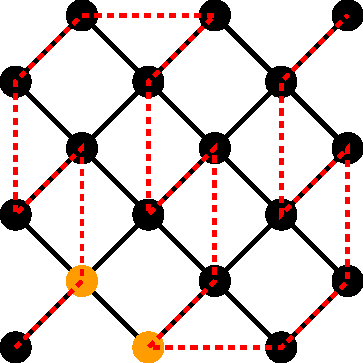
\includegraphics[scale=0.6]{figures/tikz/TFI/dmrg_snaking/dmrg_snaking.pdf}
	\caption{An MPS can be put on a 2D square lattice by "snaking" it through the lattice. The two sites marked in orange are nearest neighbour sites in the lattice, but are far apart in the MPS. Thus, entanglement between the two sites is hard to represent, requiring large bond dimensions.}
	\label{fig:tenpy_snaking}
\end{figure}

\section{The Transverse Field Ising Model}
\label{sec:TFI_model}
The Transverse Field Ising (TFI) model is a well-studied spin lattice model that is described by the Hamiltonian
\begin{equation}
	\label{eq:TFI_Hamiltonian}
	\hat{H}_\text{TFI} = -J\sum_{\langle i,j\rangle} \hat{\sigma}^x_i \hat{\sigma}^x_j - g\sum_{i} \hat{\sigma}^z_i,
\end{equation}
where $\langle i,j\rangle$ denotes pairs of nearest neighbours and $\hat{\sigma}^x_i, \hat{\sigma}^z_i$ are the Pauli matrices. The model is widely used for benchmarking numerical methods. Here we will only discuss the TFI model on a two-dimensional lattice, which can be mapped to a classical Ising model on a three-dimensional lattice \cite{cite:from_d_dimensional_quantum_to_dp1_dimensional_classical}. We will further restrict ourselves to the ferromagnetic case $J > 0$ and to zero temperature. In the limit of vanishing transverse field $g \rightarrow 0$ the model reduces to a classical 2D Ising model. The ground state is degenerate with all spins pointing either up or down in the $S^x$ direction. The associated phase is the classically disordered phase \cite{cite:critical_behavior_of_the_two_dim_ising_model_in_transverse_field, cite:quantum_ising_phases_and_transitions_in_transverse_ising_models}, or ferromagnetic phase. Taking the other limit, $g \gg J$, reduces the model to non-interacting spins in an external field. The ground state is unique with all spins pointing in $S^z$ direction. The corresponding phase is called the paramagnetic phase. There exists a quantum phase transition at a critical transverse field $g = g_\text{C}$ from the ferromagnetic to the paramagnetic phase. Blöte and Deng computed the value of the critical field for the TFI model on the square lattice as $g \approx 3.04438$ using Quantum Monte Carlo methods \cite{cite:cluster_monte_carlo_simulation_of_TFI}. \par
In the following we benchmark disoTPS methods on the TFI model. We first perform ground state searches using imaginary time evolution in section \ref{sec:TFI_ground_state_search}. We benchmark the different proposed algorithms for the YB move and compare the first and second order TEBD algorithms. We further show numerical evidence that disoTPS are able to capture area law entanglement. Lastly we perform a ground state search on the honeycomb lattice, showing that disoTPS is easily generalized to different lattice types. In seciont \ref{sec:TFI_time_evolution} we perform a global quench and compute real time evolution. We observe that disoTPS struggles with the rapid entanglement growth and discuss some ideas for overcoming the problem. \par
We compare the results obtained with disoTPS to reference DMRG simulations using the tenpy library \cite{cite:tenpy}. The DMRG simulations are performed by "snaking" an MPS through the 2D lattice as shown in figure \figref{fig:tenpy_snaking}. The disadvantage of this method is that sites that are close to each other in the lattice can be far apart in the MPS. Because of the close proximity of these sites we expect entanglement to build up between them. This entanglement cannot be captured well by the MPS because of its finite bond dimension, which is only able to capture entanglement locally in the MPS. We thus expect DMRG to break down for large systems. However, because of the low computational complexity of DMRG, one can scale the bond dimension to large values. For the lattice sizes we looked at this still allows for accurate results.
\begin{figure}
\centering
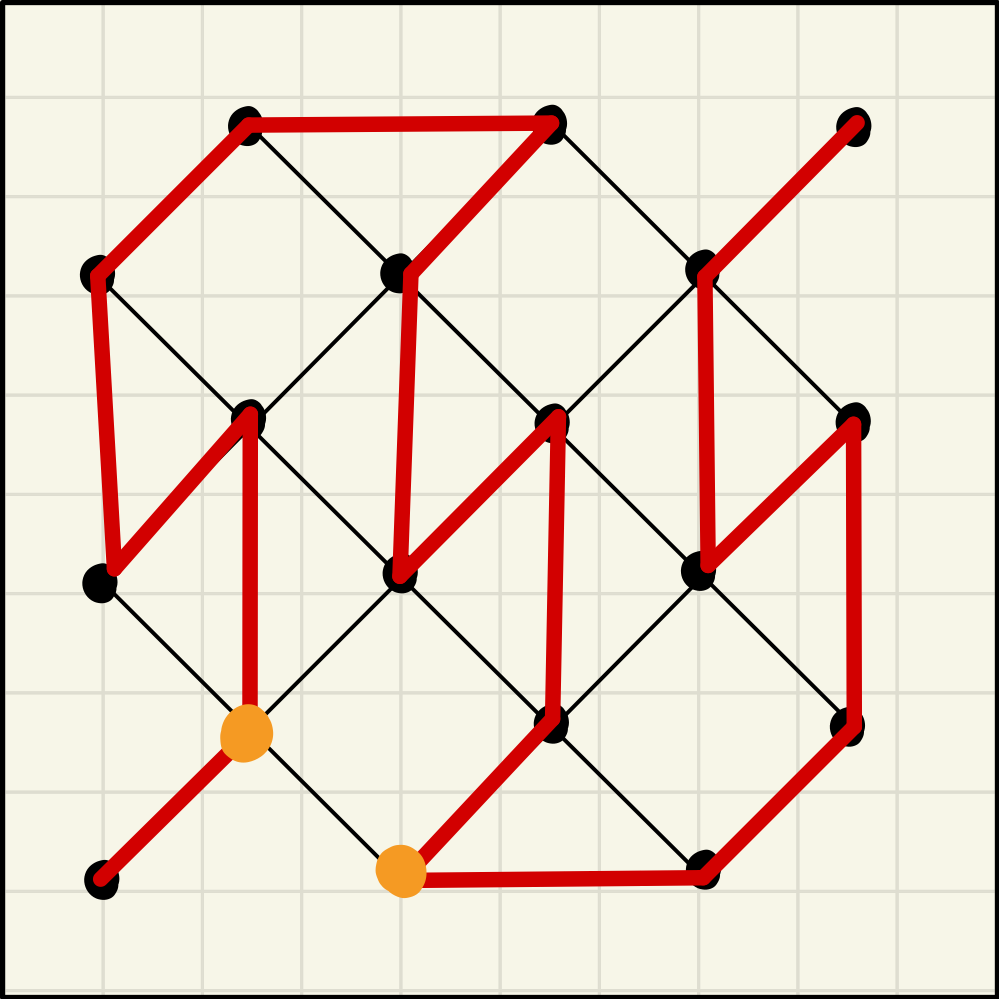
\includegraphics[width=0.4\textwidth]{figures/TFI/tenpy_snaking.jpeg}
\caption{An MPS can be put on a 2D square lattice by "snaking" it through the lattice. The two sites marked in orange are nearest neighbour sites in the lattice, but are far apart in the MPS. Thus, entanglement between the two sites is hard to represent, requiring large bond dimensions.}
\label{fig:tenpy_snaking}
\end{figure}


\section{Ground State Search}
\label{sec:TFI_ground_state_search}
\begin{figure}
	\centering
	\begin{minipage}{1.0\textwidth}
		\centering
		\begin{tikzpicture}[scale=1, trim axis left, trim axis right]
			\begin{axis}[ylabel={$\Delta E / E_\text{exact}$}, grid=both, grid style={gray!20}, every axis plot/.append style={very thick}, scale only axis, height=\gsEnergyVsDtauFigureHeight, width=\gsEnergyVsDtauFigureWidth, xmode=log, ymode=log, ymin=1e-6, ymax=1e-1, legend style={nodes={scale=\legendscale, transform shape, font=\small}}, legend pos=south west, title={\footnotesize\textbf{SVD}}, xticklabels={}, legend cell align={left}]
				%	
				\addplot[color = 3blue1, mark=*]
				table[x=dtau, y=delta_E_D_max_2, col sep=space]{figures/plots/TFI/gs_energy_vs_dtau/data/gs_energy_vs_dtau_square_svd.txt};
				\addlegendentry{$D = 2$}
				%	
				\addplot[color = 3blue2, mark=*]
				table[x=dtau, y=delta_E_D_max_4, col sep=space]{figures/plots/TFI/gs_energy_vs_dtau/data/gs_energy_vs_dtau_square_svd.txt};
				\addlegendentry{$D = 4$}
				%	
				\addplot[color = 3blue3, mark=*]
				table[x=dtau, y=delta_E_D_max_6, col sep=space]{figures/plots/TFI/gs_energy_vs_dtau/data/gs_energy_vs_dtau_square_svd.txt};
				\addlegendentry{$D = 6$}
			\end{axis}%
		\end{tikzpicture}%
		\,\,
		\begin{tikzpicture}[scale=1, trim axis left, trim axis right]
			\begin{axis}[grid=both, grid style={gray!20}, every axis plot/.append style={very thick}, scale only axis, height=\gsEnergyVsDtauFigureHeight, width=\gsEnergyVsDtauFigureWidth, xmode=log, ymode=log, ymin=1e-6, ymax=1e-1, yticklabels={}, title={\footnotesize\textbf{SVD + init}}, xticklabels={}]
				%	
				\addplot[color = 3blue1, mark=*]
				table[x=dtau, y=delta_E_D_max_2, col sep=space]{figures/plots/TFI/gs_energy_vs_dtau/data/gs_energy_vs_dtau_square_svd_init_polar.txt};
				%\addlegendentry{$D = 2$}
				%	
				\addplot[color = 3blue2, mark=*]
				table[x=dtau, y=delta_E_D_max_4, col sep=space]{figures/plots/TFI/gs_energy_vs_dtau/data/gs_energy_vs_dtau_square_svd_init_polar.txt};
				%\addlegendentry{$D = 4$}
				%	
				\addplot[color = 3blue3, mark=*]
				table[x=dtau, y=delta_E_D_max_6, col sep=space]{figures/plots/TFI/gs_energy_vs_dtau/data/gs_energy_vs_dtau_square_svd_init_polar.txt};
				%\addlegendentry{$D = 6$}
			\end{axis}%
		\end{tikzpicture}%
		\,\,
		\begin{tikzpicture}[scale=1, trim axis left, trim axis right]
			\begin{axis}[grid=both, grid style={gray!20}, every axis plot/.append style={very thick}, scale only axis, height=\gsEnergyVsDtauFigureHeight, width=\gsEnergyVsDtauFigureWidth, xmode=log, ymode=log, ymin=1e-6, ymax=1e-1, yticklabels={}, title={\footnotesize\textbf{EV trunc}}, xticklabels={}]
				%	
				\addplot[color = 3blue1, mark=*]
				table[x=dtau, y=delta_E_D_max_2, col sep=space]{figures/plots/TFI/gs_energy_vs_dtau/data/gs_energy_vs_dtau_square_iterate_polar.txt};
				%\addlegendentry{$D = 2$}
				%	
				\addplot[color = 3blue2, mark=*]
				table[x=dtau, y=delta_E_D_max_4, col sep=space]{figures/plots/TFI/gs_energy_vs_dtau/data/gs_energy_vs_dtau_square_iterate_polar.txt};
				%\addlegendentry{$D = 4$}
				%	
				\addplot[color = 3blue3, mark=*]
				table[x=dtau, y=delta_E_D_max_6, col sep=space]{figures/plots/TFI/gs_energy_vs_dtau/data/gs_energy_vs_dtau_square_iterate_polar.txt};
				%\addlegendentry{$D = 6$}
			\end{axis}%
		\end{tikzpicture}%
		\,\,
		\begin{tikzpicture}[scale=1, trim axis left, trim axis right]
			\begin{axis}[grid=both, grid style={gray!20}, every axis plot/.append style={very thick}, scale only axis, height=\gsEnergyVsDtauFigureHeight, width=\gsEnergyVsDtauFigureWidth, xmode=log, ymode=log, ymin=1e-6, ymax=1e-1, yticklabels={}, title={\footnotesize\textbf{EV Rényi-2}}, xticklabels={}]
				%	
				\addplot[color = 3blue1, mark=*]
				table[x=dtau, y=delta_E_D_max_2, col sep=space]{figures/plots/TFI/gs_energy_vs_dtau/data/gs_energy_vs_dtau_square_svd_disent_renyi_2.0_power_iteration.txt};
				%\addlegendentry{$D = 2$}
				%	
				\addplot[color = 3blue2, mark=*]
				table[x=dtau, y=delta_E_D_max_4, col sep=space]{figures/plots/TFI/gs_energy_vs_dtau/data/gs_energy_vs_dtau_square_svd_disent_renyi_2.0_power_iteration.txt};
				%\addlegendentry{$D = 4$}
				%	
				\addplot[color = 3blue3, mark=*]
				table[x=dtau, y=delta_E_D_max_6, col sep=space]{figures/plots/TFI/gs_energy_vs_dtau/data/gs_energy_vs_dtau_square_svd_disent_renyi_2.0_power_iteration.txt};
				%\addlegendentry{$D = 6$}
			\end{axis}%
		\end{tikzpicture}%
	\end{minipage}
	\begin{minipage}{1.0\textwidth}
		\centering%
		% ====================================================================================
		% 2nd line
		% ====================================================================================
		\begin{tikzpicture}[scale=1, trim axis left, trim axis right]
			\begin{axis}[ylabel={$\Delta E / E_\text{exact}$}, grid=both, grid style={gray!20}, every axis plot/.append style={very thick}, scale only axis, height=\gsEnergyVsDtauFigureHeight, width=\gsEnergyVsDtauFigureWidth, xmode=log, ymode=log, ymin=1e-6, ymax=1e-1, title={\footnotesize\textbf{CG trunc}}, xticklabels={}]
				%	
				\addplot[color = 3blue1, mark=*]
				table[x=dtau, y=delta_E_D_max_2, col sep=space]{figures/plots/TFI/gs_energy_vs_dtau/data/gs_energy_vs_dtau_square_svd_disent_trunc_error_cg.txt};
				%\addlegendentry{$D = 2$}
				%	
				\addplot[color = 3blue2, mark=*]
				table[x=dtau, y=delta_E_D_max_4, col sep=space]{figures/plots/TFI/gs_energy_vs_dtau/data/gs_energy_vs_dtau_square_svd_disent_trunc_error_cg.txt};
				%\addlegendentry{$D = 4$}
				%	
				\addplot[color = 3blue3, mark=*]
				table[x=dtau, y=delta_E_D_max_6, col sep=space]{figures/plots/TFI/gs_energy_vs_dtau/data/gs_energy_vs_dtau_square_svd_disent_trunc_error_cg.txt};
				%\addlegendentry{$D = 6$}
			\end{axis}%
		\end{tikzpicture}%
		\,\,
		\begin{tikzpicture}[scale=1, trim axis left, trim axis right]
			\begin{axis}[grid=both, grid style={gray!20}, every axis plot/.append style={very thick}, scale only axis, height=\gsEnergyVsDtauFigureHeight, width=\gsEnergyVsDtauFigureWidth, xmode=log, ymode=log, ymin=1e-6, ymax=1e-1, yticklabels={}, title={\footnotesize\textbf{approx CG trunc}}, xticklabels={}]
				%	
				\addplot[color = 3blue1, mark=*]
				table[x=dtau, y=delta_E_D_max_2, col sep=space]{figures/plots/TFI/gs_energy_vs_dtau/data/gs_energy_vs_dtau_square_svd_disent_trunc_error_approx_cg.txt};
				%\addlegendentry{$D = 2$}
				%	
				\addplot[color = 3blue2, mark=*]
				table[x=dtau, y=delta_E_D_max_4, col sep=space]{figures/plots/TFI/gs_energy_vs_dtau/data/gs_energy_vs_dtau_square_svd_disent_trunc_error_approx_cg.txt};
				%\addlegendentry{$D = 4$}
				%	
				\addplot[color = 3blue3, mark=*]
				table[x=dtau, y=delta_E_D_max_6, col sep=space]{figures/plots/TFI/gs_energy_vs_dtau/data/gs_energy_vs_dtau_square_svd_disent_trunc_error_approx_cg.txt};
				%\addlegendentry{$D = 6$}
			\end{axis}%
		\end{tikzpicture}%
		\,\,
		\begin{tikzpicture}[scale=1, trim axis left, trim axis right]
			\begin{axis}[grid=both, grid style={gray!20}, every axis plot/.append style={very thick}, scale only axis, height=\gsEnergyVsDtauFigureHeight, width=\gsEnergyVsDtauFigureWidth, xmode=log, ymode=log, ymin=1e-6, ymax=1e-1, yticklabels={}, title={\footnotesize\textbf{TRM trunc}}, xticklabels={}]
				%	
				\addplot[color = 3blue1, mark=*]
				table[x=dtau, y=delta_E_D_max_2, col sep=space]{figures/plots/TFI/gs_energy_vs_dtau/data/gs_energy_vs_dtau_square_svd_disent_trunc_error_trm.txt};
				%\addlegendentry{$D = 2$}
				%	
				\addplot[color = 3blue2, mark=*]
				table[x=dtau, y=delta_E_D_max_4, col sep=space]{figures/plots/TFI/gs_energy_vs_dtau/data/gs_energy_vs_dtau_square_svd_disent_trunc_error_trm.txt};
				%\addlegendentry{$D = 4$}
				%	
				\addplot[color = 3blue3, mark=*]
				table[x=dtau, y=delta_E_D_max_6, col sep=space]{figures/plots/TFI/gs_energy_vs_dtau/data/gs_energy_vs_dtau_square_svd_disent_trunc_error_trm.txt};
				%\addlegendentry{$D = 6$}
			\end{axis}%
		\end{tikzpicture}%
		\,\,
		\begin{tikzpicture}[scale=1, trim axis left, trim axis right]
			\begin{axis}[grid=both, grid style={gray!20}, every axis plot/.append style={very thick}, scale only axis, height=\gsEnergyVsDtauFigureHeight, width=\gsEnergyVsDtauFigureWidth, xmode=log, ymode=log, ymin=1e-6, ymax=1e-1, yticklabels={}, title={\footnotesize\textbf{approx TRM trunc}}, xticklabels={}]
				%	
				\addplot[color = 3blue1, mark=*]
				table[x=dtau, y=delta_E_D_max_2, col sep=space]{figures/plots/TFI/gs_energy_vs_dtau/data/gs_energy_vs_dtau_square_svd_disent_trunc_error_approx_trm.txt};
				%\addlegendentry{$D = 2$}
				%	
				\addplot[color = 3blue2, mark=*]
				table[x=dtau, y=delta_E_D_max_4, col sep=space]{figures/plots/TFI/gs_energy_vs_dtau/data/gs_energy_vs_dtau_square_svd_disent_trunc_error_approx_trm.txt};
				%\addlegendentry{$D = 4$}
				%	
				\addplot[color = 3blue3, mark=*]
				table[x=dtau, y=delta_E_D_max_6, col sep=space]{figures/plots/TFI/gs_energy_vs_dtau/data/gs_energy_vs_dtau_square_svd_disent_trunc_error_approx_trm.txt};
				%\addlegendentry{$D = 6$}
			\end{axis}%
		\end{tikzpicture}%
	\end{minipage}
	\begin{minipage}{1.0\textwidth}
		\centering%
		% ====================================================================================
		% 3rd line
		% ====================================================================================
		\begin{tikzpicture}[scale=1, trim axis left, trim axis right]
			\begin{axis}[xlabel=$\Delta\tau$, ylabel={$\Delta E / E_\text{exact}$}, grid=both, grid style={gray!20}, every axis plot/.append style={very thick}, scale only axis, height=\gsEnergyVsDtauFigureHeight, width=\gsEnergyVsDtauFigureWidth, xmode=log, ymode=log, ymin=1e-6, ymax=1e-1, title={\footnotesize\textbf{CG Rényi-0.5}}]
				%	
				\addplot[color = 3blue1, mark=*]
				table[x=dtau, y=delta_E_D_max_2, col sep=space]{figures/plots/TFI/gs_energy_vs_dtau/data/gs_energy_vs_dtau_square_svd_disent_renyi_0.5_cg.txt};
				%\addlegendentry{$D = 2$}
				%	
				\addplot[color = 3blue2, mark=*]
				table[x=dtau, y=delta_E_D_max_4, col sep=space]{figures/plots/TFI/gs_energy_vs_dtau/data/gs_energy_vs_dtau_square_svd_disent_renyi_0.5_cg.txt};
				%\addlegendentry{$D = 4$}
				%	
				\addplot[color = 3blue3, mark=*]
				table[x=dtau, y=delta_E_D_max_6, col sep=space]{figures/plots/TFI/gs_energy_vs_dtau/data/gs_energy_vs_dtau_square_svd_disent_renyi_0.5_cg.txt};
				%\addlegendentry{$D = 6$}
			\end{axis}%
		\end{tikzpicture}%
		\,\,
		\begin{tikzpicture}[scale=1, trim axis left, trim axis right]
			\begin{axis}[xlabel=$\Delta\tau$, grid=both, grid style={gray!20}, every axis plot/.append style={very thick}, scale only axis, height=\gsEnergyVsDtauFigureHeight, width=\gsEnergyVsDtauFigureWidth, xmode=log, ymode=log, ymin=1e-6, ymax=1e-1, yticklabels={}, title={\footnotesize\textbf{appr.\,CG\,Rényi-0.5}}]
				%	
				\addplot[color = 3blue1, mark=*]
				table[x=dtau, y=delta_E_D_max_2, col sep=space]{figures/plots/TFI/gs_energy_vs_dtau/data/gs_energy_vs_dtau_square_svd_disent_renyi_0.5_approx_cg.txt};
				%\addlegendentry{$D = 2$}
				%	
				\addplot[color = 3blue2, mark=*]
				table[x=dtau, y=delta_E_D_max_4, col sep=space]{figures/plots/TFI/gs_energy_vs_dtau/data/gs_energy_vs_dtau_square_svd_disent_renyi_0.5_approx_cg.txt};
				%\addlegendentry{$D = 4$}
				%	
				\addplot[color = 3blue3, mark=*]
				table[x=dtau, y=delta_E_D_max_6, col sep=space]{figures/plots/TFI/gs_energy_vs_dtau/data/gs_energy_vs_dtau_square_svd_disent_renyi_0.5_approx_cg.txt};
				%\addlegendentry{$D = 6$}
			\end{axis}%
		\end{tikzpicture}%
		\,\,
		\begin{tikzpicture}[scale=1, trim axis left, trim axis right]
			\begin{axis}[xlabel=$\Delta\tau$, grid=both, grid style={gray!20}, every axis plot/.append style={very thick}, scale only axis, height=\gsEnergyVsDtauFigureHeight, width=\gsEnergyVsDtauFigureWidth, xmode=log, ymode=log, ymin=1e-6, ymax=1e-1, yticklabels={}, title={\footnotesize\textbf{TRM\,Rényi-0.5}}]
				%	
				\addplot[color = 3blue1, mark=*]
				table[x=dtau, y=delta_E_D_max_2, col sep=space]{figures/plots/TFI/gs_energy_vs_dtau/data/gs_energy_vs_dtau_square_svd_disent_renyi_0.5_trm.txt};
				%\addlegendentry{$D = 2$}
				%	
				\addplot[color = 3blue2, mark=*]
				table[x=dtau, y=delta_E_D_max_4, col sep=space]{figures/plots/TFI/gs_energy_vs_dtau/data/gs_energy_vs_dtau_square_svd_disent_renyi_0.5_trm.txt};
				%\addlegendentry{$D = 4$}
				%	
				\addplot[color = 3blue3, mark=*]
				table[x=dtau, y=delta_E_D_max_6, col sep=space]{figures/plots/TFI/gs_energy_vs_dtau/data/gs_energy_vs_dtau_square_svd_disent_renyi_0.5_trm.txt};
				%\addlegendentry{$D = 6$}
			\end{axis}%
		\end{tikzpicture}%
		\,\,
		\begin{tikzpicture}[scale=1, trim axis left, trim axis right]
			\begin{axis}[xlabel=$\Delta\tau$, grid=both, grid style={gray!20}, every axis plot/.append style={very thick}, scale only axis, height=\gsEnergyVsDtauFigureHeight, width=\gsEnergyVsDtauFigureWidth, xmode=log, ymode=log, ymin=1e-6, ymax=1e-1, yticklabels={}, title={\footnotesize\textbf{appr.\,TRM\,Rényi-0.5}}]
				%	
				\addplot[color = 3blue1, mark=*]
				table[x=dtau, y=delta_E_D_max_2, col sep=space]{figures/plots/TFI/gs_energy_vs_dtau/data/gs_energy_vs_dtau_square_svd_disent_renyi_0.5_approx_trm.txt};
				%\addlegendentry{$D = 2$}
				%	
				\addplot[color = 3blue2, mark=*]
				table[x=dtau, y=delta_E_D_max_4, col sep=space]{figures/plots/TFI/gs_energy_vs_dtau/data/gs_energy_vs_dtau_square_svd_disent_renyi_0.5_approx_trm.txt};
				%\addlegendentry{$D = 4$}
				%	
				\addplot[color = 3blue3, mark=*]
				table[x=dtau, y=delta_E_D_max_6, col sep=space]{figures/plots/TFI/gs_energy_vs_dtau/data/gs_energy_vs_dtau_square_svd_disent_renyi_0.5_approx_trm.txt};
				%\addlegendentry{$D = 6$}
			\end{axis}%
		\end{tikzpicture}%
	\end{minipage}
	\caption{We benchmark the different implemented methods for the YB move on the TFI model on a $4\times4$ square lattice. The transverse field is set to $g = 3.5$. We compute the ground state energy with imaginary TEBD for different time step sizes $\Delta\tau$. First row: SVD splitting without disentangling, SVD splitting with a disentangling unitary initialized with an SVD as in \cite{cite:isometric_tensor_network_states_in_two_dimensions, cite:efficient_simulation_of_dynamics_in_two_dimensional_quantum_spin_systems}, Evenbly-Vidal minimization of the truncation error, and Evenbly-Vidal minimization of the Rényi-2 entropy. Second row: Disentangling with Riemannian optimization of the truncation error. Third row: Disentangling with Riemannian optimization of the  Rényi-1/2 entropy. All iterative methods were run for a maximum of $N_\text{iter} = 100$ iterations per YB move. The bond dimension of the orthogonality hypersurface was set to $\chi = 6\cdot D$.}
	\label{fig:tfi_gs_energy_vs_dtau_different_methods}
\end{figure}
\begin{figure}
	\centering
	\begin{minipage}{1.0\textwidth}
		\centering
		\begin{tikzpicture}[scale=1, trim axis left, trim axis right]
			\begin{axis}[xlabel=$\text{d}\tau$, ylabel={$\Delta E / E_\text{exact}$}, grid=both, grid style={gray!20}, every axis plot/.append style={very thick}, scale only axis, height=\gsEnergyVsDtauFigureHeight, width=\gsEnergyVsDtauFigureWidth, xmode=log, ymode=log, ymin=1e-6, ymax=1e-1, title={$N_\text{iters} = 1$}]
				%	
				\addplot[color = 3blue1, mark=*]
				table[x=dtau, y=delta_E_D_max_2, col sep=space]{figures/plots/TFI/gs_energy_vs_dtau/data/gs_energy_vs_dtau_square_svd_disent_renyi_0.5_approx_trm_N_iters_1.txt};
				%\addlegendentry{$D = 2$}
				%	
				\addplot[color = 3blue2, mark=*]
				table[x=dtau, y=delta_E_D_max_4, col sep=space]{figures/plots/TFI/gs_energy_vs_dtau/data/gs_energy_vs_dtau_square_svd_disent_renyi_0.5_approx_trm_N_iters_1.txt};
				%\addlegendentry{$D = 4$}
				%	
				\addplot[color = 3blue3, mark=*]
				table[x=dtau, y=delta_E_D_max_6, col sep=space]{figures/plots/TFI/gs_energy_vs_dtau/data/gs_energy_vs_dtau_square_svd_disent_renyi_0.5_approx_trm_N_iters_1.txt};
				%\addlegendentry{$D = 6$}
			\end{axis}%
		\end{tikzpicture}%
		\,\,
		\begin{tikzpicture}[scale=1, trim axis left, trim axis right]
			\begin{axis}[xlabel=$\text{d}\tau$, grid=both, grid style={gray!20}, every axis plot/.append style={very thick}, scale only axis, height=\gsEnergyVsDtauFigureHeight, width=\gsEnergyVsDtauFigureWidth, xmode=log, ymode=log, ymin=1e-6, ymax=1e-1, yticklabels={}, title={$N_\text{iters} = 10$}]
				%	
				\addplot[color = 3blue1, mark=*]
				table[x=dtau, y=delta_E_D_max_2, col sep=space]{figures/plots/TFI/gs_energy_vs_dtau/data/gs_energy_vs_dtau_square_svd_disent_renyi_0.5_approx_trm_N_iters_10.txt};
				%\addlegendentry{$D = 2$}
				%	
				\addplot[color = 3blue2, mark=*]
				table[x=dtau, y=delta_E_D_max_4, col sep=space]{figures/plots/TFI/gs_energy_vs_dtau/data/gs_energy_vs_dtau_square_svd_disent_renyi_0.5_approx_trm_N_iters_10.txt};
				%\addlegendentry{$D = 4$}
				%	
				\addplot[color = 3blue3, mark=*]
				table[x=dtau, y=delta_E_D_max_6, col sep=space]{figures/plots/TFI/gs_energy_vs_dtau/data/gs_energy_vs_dtau_square_svd_disent_renyi_0.5_approx_trm_N_iters_10.txt};
				%\addlegendentry{$D = 6$}
			\end{axis}%
		\end{tikzpicture}%
		\,\,
		\begin{tikzpicture}[scale=1, trim axis left, trim axis right]
			\begin{axis}[xlabel=$\text{d}\tau$, grid=both, grid style={gray!20}, every axis plot/.append style={very thick}, scale only axis, height=\gsEnergyVsDtauFigureHeight, width=\gsEnergyVsDtauFigureWidth, xmode=log, ymode=log, ymin=1e-6, ymax=1e-1, yticklabels={}, title={$N_\text{iters} = 50$}]
				%	
				\addplot[color = 3blue1, mark=*]
				table[x=dtau, y=delta_E_D_max_2, col sep=space]{figures/plots/TFI/gs_energy_vs_dtau/data/gs_energy_vs_dtau_square_svd_disent_renyi_0.5_approx_trm_N_iters_50.txt};
				%\addlegendentry{$D = 2$}
				%	
				\addplot[color = 3blue2, mark=*]
				table[x=dtau, y=delta_E_D_max_4, col sep=space]{figures/plots/TFI/gs_energy_vs_dtau/data/gs_energy_vs_dtau_square_svd_disent_renyi_0.5_approx_trm_N_iters_50.txt};
				%\addlegendentry{$D = 4$}
				%	
				\addplot[color = 3blue3, mark=*]
				table[x=dtau, y=delta_E_D_max_6, col sep=space]{figures/plots/TFI/gs_energy_vs_dtau/data/gs_energy_vs_dtau_square_svd_disent_renyi_0.5_approx_trm_N_iters_50.txt};
				%\addlegendentry{$D = 6$}
			\end{axis}%
		\end{tikzpicture}%
		\,\,
		\begin{tikzpicture}[scale=1, trim axis left, trim axis right]
			\begin{axis}[xlabel=$\text{d}\tau$, grid=both, grid style={gray!20}, every axis plot/.append style={very thick}, scale only axis, height=\gsEnergyVsDtauFigureHeight, width=\gsEnergyVsDtauFigureWidth, xmode=log, ymode=log, ymin=1e-6, ymax=1e-1, yticklabels={}, title={$N_\text{iters} = 200$}, legend style={nodes={scale=\legendscale, transform shape}}, legend pos=north west]
				%	
				\addplot[color = 3blue1, mark=*]
				table[x=dtau, y=delta_E_D_max_2, col sep=space]{figures/plots/TFI/gs_energy_vs_dtau/data/gs_energy_vs_dtau_square_svd_disent_renyi_0.5_approx_trm_N_iters_200.txt};
				\addlegendentry{$D = 2$}
				%	
				\addplot[color = 3blue2, mark=*]
				table[x=dtau, y=delta_E_D_max_4, col sep=space]{figures/plots/TFI/gs_energy_vs_dtau/data/gs_energy_vs_dtau_square_svd_disent_renyi_0.5_approx_trm_N_iters_200.txt};
				\addlegendentry{$D = 4$}
				%	
				\addplot[color = 3blue3, mark=*]
				table[x=dtau, y=delta_E_D_max_6, col sep=space]{figures/plots/TFI/gs_energy_vs_dtau/data/gs_energy_vs_dtau_square_svd_disent_renyi_0.5_approx_trm_N_iters_200.txt};
				\addlegendentry{$D = 6$}
			\end{axis}%
		\end{tikzpicture}%
	\end{minipage}
	\caption{In this figure we test how many iterations of Riemannian optimization are necessary for the approximate TRM algorithm minimizing the Rényi-$0.5$ entropy to converge. As a model we use the TFI model on a $4\times4$ suare lattice with a transverse field of $g = 3.5$. The bond dimension of the orthogonality hypersurface is set to $\chi=6\cdot D$. We compute the ground state energy with imaginary TEBD for different time step sizes $\text{d}\tau$.}
	\label{fig:tfi_gs_energy_vs_dtau_different_N_iters}
\end{figure}
\begin{figure}
	\centering
	\begin{tikzpicture}[scale=1, trim axis left, trim axis right]
		\begin{axis}[xlabel=$\text{d}\tau$, ylabel={$\Delta E / E_\text{exact}$}, grid=both, grid style={gray!20}, every axis plot/.append style={very thick}, scale only axis, height=\gsEnergyVsDtauFigureHeight, width=\gsEnergyVsDtauFigureWidth, xmode=log, ymode=log, ymin=1e-6, ymax=1e-1, title={TEBD1}]
			%	
			\addplot[color = 3blue1, mark=*]
			table[x=dtau, y=delta_E_D_max_2, col sep=space]{figures/plots/TFI/gs_energy_vs_dtau/data/gs_energy_vs_dtau_square_svd_disent_renyi_0.5_approx_trm_tebd1.txt};
			%\addlegendentry{$D = 2$}
			%	
			\addplot[color = 3blue2, mark=*]
			table[x=dtau, y=delta_E_D_max_4, col sep=space]{figures/plots/TFI/gs_energy_vs_dtau/data/gs_energy_vs_dtau_square_svd_disent_renyi_0.5_approx_trm_tebd1.txt};
			%\addlegendentry{$D = 4$}
			%	
			\addplot[color = 3blue3, mark=*]
			table[x=dtau, y=delta_E_D_max_6, col sep=space]{figures/plots/TFI/gs_energy_vs_dtau/data/gs_energy_vs_dtau_square_svd_disent_renyi_0.5_approx_trm_tebd1.txt};
			%\addlegendentry{$D = 6$}
		\end{axis}%
	\end{tikzpicture}%
	\,\,
	\begin{tikzpicture}[scale=1, trim axis left, trim axis right]
		\begin{axis}[xlabel=$\text{d}\tau$, grid=both, grid style={gray!20}, every axis plot/.append style={very thick}, scale only axis, height=\gsEnergyVsDtauFigureHeight, width=\gsEnergyVsDtauFigureWidth, xmode=log, ymode=log, ymin=1e-6, ymax=1e-1, yticklabels={}, title={TEBD2}, legend style={nodes={scale=\legendscale, transform shape}}]
			%	
			\addplot[color = 3blue1, mark=*]
			table[x=dtau, y=delta_E_D_max_2, col sep=space]{figures/plots/TFI/gs_energy_vs_dtau/data/gs_energy_vs_dtau_square_svd_disent_renyi_0.5_approx_trm_tebd2.txt};
			\addlegendentry{$D = 2$}
			%	
			\addplot[color = 3blue2, mark=*]
			table[x=dtau, y=delta_E_D_max_4, col sep=space]{figures/plots/TFI/gs_energy_vs_dtau/data/gs_energy_vs_dtau_square_svd_disent_renyi_0.5_approx_trm_tebd2.txt};
			\addlegendentry{$D = 4$}
			%	
			\addplot[color = 3blue3, mark=*]
			table[x=dtau, y=delta_E_D_max_6, col sep=space]{figures/plots/TFI/gs_energy_vs_dtau/data/gs_energy_vs_dtau_square_svd_disent_renyi_0.5_approx_trm_tebd2.txt};
			\addlegendentry{$D = 6$}
		\end{axis}%
	\end{tikzpicture}%
	\caption{\todo{Caption}}
	\label{fig:tfi_gs_energy_vs_dtau_TEBD1_vs_TEBD2}
\end{figure}
\begin{figure}
	\centering
	\begin{minipage}{1.0\textwidth}
		\centering
		\begin{tikzpicture}[scale=1, trim axis left, trim axis right]
			\begin{axis}[xlabel=$\Delta\tau$, ylabel={$\Delta E / E_\text{exact}$}, grid=both, grid style={gray!20}, every axis plot/.append style={very thick}, scale only axis, height=\gsEnergyVsDtauFigureHeight, width=\gsEnergyVsDtauFigureWidth, xmode=log, ymode=log, ymin=1e-6, ymax=1e-1, title={$D_\text{horizontal} = D$}]
				%	
				\addplot[color = 3blue1, mark=*]
				table[x=dtau, y=delta_E_D_max_2, col sep=space]{figures/plots/TFI/gs_energy_vs_dtau/data/gs_energy_vs_dtau_honeycomb_svd_disent_renyi_0.5_approx_trm_D_horizontal_equal_D.txt};
				%\addlegendentry{$D = 2$}
				%	
				\addplot[color = 3blue2, mark=*]
				table[x=dtau, y=delta_E_D_max_4, col sep=space]{figures/plots/TFI/gs_energy_vs_dtau/data/gs_energy_vs_dtau_honeycomb_svd_disent_renyi_0.5_approx_trm_D_horizontal_equal_D.txt};
				%\addlegendentry{$D = 4$}
				%	
				\addplot[color = 3blue3, mark=*]
				table[x=dtau, y=delta_E_D_max_6, col sep=space]{figures/plots/TFI/gs_energy_vs_dtau/data/gs_energy_vs_dtau_honeycomb_svd_disent_renyi_0.5_approx_trm_D_horizontal_equal_D.txt};
				%\addlegendentry{$D = 6$}
			\end{axis}%
		\end{tikzpicture}%
		\,\,
		\begin{tikzpicture}[scale=1, trim axis left, trim axis right]
			\begin{axis}[xlabel=$\Delta\tau$, grid=both, grid style={gray!20}, every axis plot/.append style={very thick}, scale only axis, height=\gsEnergyVsDtauFigureHeight, width=\gsEnergyVsDtauFigureWidth, xmode=log, ymode=log, ymin=1e-6, ymax=1e-1, yticklabels={}, title={$D_\text{horizontal} = D^2$}, legend style={nodes={scale=\legendscale, transform shape, font=\small}}]
				%	
				\addplot[color = 3blue1, mark=*]
				table[x=dtau, y=delta_E_D_max_2, col sep=space]{figures/plots/TFI/gs_energy_vs_dtau/data/gs_energy_vs_dtau_honeycomb_svd_disent_renyi_0.5_approx_trm_D_horizontal_equal_D_squared.txt};
				\addlegendentry{$D = 2$}
				%	
				\addplot[color = 3blue2, mark=*]
				table[x=dtau, y=delta_E_D_max_4, col sep=space]{figures/plots/TFI/gs_energy_vs_dtau/data/gs_energy_vs_dtau_honeycomb_svd_disent_renyi_0.5_approx_trm_D_horizontal_equal_D_squared.txt};
				\addlegendentry{$D = 4$}
				%	
				\addplot[color = 3blue3, mark=*]
				table[x=dtau, y=delta_E_D_max_6, col sep=space]{figures/plots/TFI/gs_energy_vs_dtau/data/gs_energy_vs_dtau_honeycomb_svd_disent_renyi_0.5_approx_trm_D_horizontal_equal_D_squared.txt};
				\addlegendentry{$D = 6$}
			\end{axis}%
		\end{tikzpicture}%
		\quad\quad
		\raisebox{15pt}
		{%
			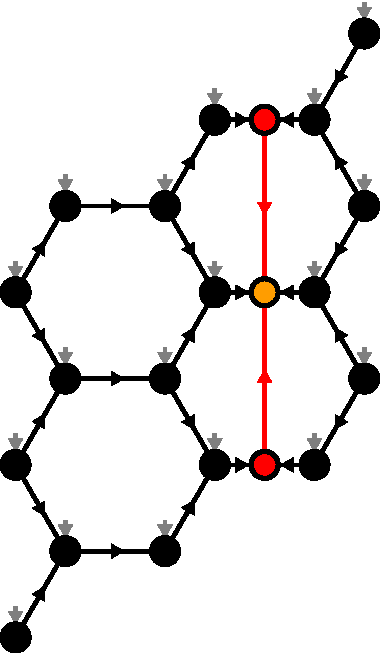
\includegraphics[scale=0.5]{figures/tikz/TFI/hexagonal_lattice/hexagonal_lattice_structure.pdf}
		}
	\end{minipage}
	\caption{In this figure we show imaginary TEBD results using disoTPS on the honeycomb lattice. We used two different values for the horizontal bond dimension, $D_\text{horizontal} = D$ and $D_\text{horizontal} = D^2$. The bond dimension along the orthogonality hypersurface was chosen as $\chi = 6\cdot D$. For the YB move we used the approximate Rényi-$0.5$ disentangler with a maximum of $N_\text{iter} = 100$ iterations per YB move. The model is the TFI model on a $4\times 4$ honeycomb lattice at a transverse field of $g = 3.5$. On the right we show the disoTPS structure of a $3\times 3$ honeycomb lattice as comparison.}
	\label{fig:tfi_gs_energy_vs_dtau_honeycomb}
\end{figure}
%\usetikzlibrary{backgrounds} % DEBUG
%background rectangle/.style={fill=olive!45}, show background rectangle
\begin{figure}
	\centering
	\begin{minipage}{1.0\textwidth}
		\hspace{280pt}
		\begin{tikzpicture}[scale=1, trim axis left, trim axis right]
			\begin{axis}[xlabel=$L$, ylabel={$E/N$}, grid=both, grid style={gray!20}, every axis plot/.append style={very thick}, scale only axis, height=\singleFigureHeight, width=\singleFigureWidth, ymin=-3.655, ymax=-3.565, legend style={at={(0.985,0.9)}, anchor=north east, font=\small, nodes={scale=\legendscale, transform shape}, label={[font=\small]above:{MPS DMRG}}}, legend columns=2, xmin=1, xmax=21, legend cell align={left}]
				%	
				\addplot[color = 7blue1]
				table[x=L, y=energy_density_tenpy_chi_16, col sep=space]{figures/plots/TFI/gs_search/data/gs_search_energy_density_vs_system_size.txt};
				\addlegendentry{$\chi = 16$}
				%
				\addplot[color = 7blue2]
				table[x=L, y=energy_density_tenpy_chi_32, col sep=space]{figures/plots/TFI/gs_search/data/gs_search_energy_density_vs_system_size.txt};
				\addlegendentry{$\chi = 32$}
				%
				\addplot[color = 7blue3]
				table[x=L, y=energy_density_tenpy_chi_64, col sep=space]{figures/plots/TFI/gs_search/data/gs_search_energy_density_vs_system_size.txt};
				\addlegendentry{$\chi = 64$}
				%
				\addplot[color = 7blue4]
				table[x=L, y=energy_density_tenpy_chi_128, col sep=space]{figures/plots/TFI/gs_search/data/gs_search_energy_density_vs_system_size.txt};
				\addlegendentry{$\chi = 128$}
				%
				\addplot[color = 7blue5]
				table[x=L, y=energy_density_tenpy_chi_256, col sep=space]{figures/plots/TFI/gs_search/data/gs_search_energy_density_vs_system_size.txt};
				\addlegendentry{$\chi = 256$}
				%
				\addplot[color = 7blue6]
				table[x=L, y=energy_density_tenpy_chi_512, col sep=space]{figures/plots/TFI/gs_search/data/gs_search_energy_density_vs_system_size.txt};
				\addlegendentry{$\chi = 512$}
				%
				\addplot[color = 7blue7]
				table[x=L, y=energy_density_tenpy_chi_1024, col sep=space]{figures/plots/TFI/gs_search/data/gs_search_energy_density_vs_system_size.txt};
				\addlegendentry{$\chi = 1024$}
				%
				\addplot[color = black]
				table[x=L, y=energy_density_tenpy_extrapolated, col sep=space]{figures/plots/TFI/gs_search/data/gs_search_energy_density_vs_system_size.txt};
				\addlegendentry{$\chi \rightarrow \infty$}
				%
			\end{axis}
			\begin{axis}[every axis plot/.append style={thick}, scale only axis, height=\singleFigureHeight, width=\singleFigureWidth, ymin=-3.655, ymax=-3.565, legend style={at={(0.42,0.9)}, anchor=north east, font=\small, nodes={scale=\legendscale, transform shape}, label={[font=\small]above:{YB-isoTPS}}}, legend columns=1, xmin=1, xmax=21, clip mode=individual, legend cell align={left}, yticklabels=\empty]
				%
				\addplot[color = 4red1, mark=*]
				table[x=L, y=energy_density_isoTPS_D_2, col sep=space]{figures/plots/TFI/gs_search/data/gs_search_energy_density_vs_system_size.txt};
				\addlegendentry{$D = 2$}
				%
				\addplot[color = 4red2, mark=*]
				table[x=L, y=energy_density_isoTPS_D_3, col sep=space]{figures/plots/TFI/gs_search/data/gs_search_energy_density_vs_system_size.txt};
				\addlegendentry{$D = 3$}
				%
				\addplot[color = 4red3, mark=*]
				table[x=L, y=energy_density_isoTPS_D_4, col sep=space]{figures/plots/TFI/gs_search/data/gs_search_energy_density_vs_system_size.txt};
				\addlegendentry{$D = 4$}
				%
				\addplot[color = 4red4, mark=*]
				table[x=L, y=energy_density_isoTPS_D_5, col sep=space]{figures/plots/TFI/gs_search/data/gs_search_energy_density_vs_system_size.txt};
				\addlegendentry{$D = 5$}
				%
				\draw[thick, black] (axis cs:16,-3.65) -- (axis cs:20,-3.65) -- (axis cs:20,-3.64) -- (axis cs:16,-3.64) -- (axis cs:16,-3.65);
				\draw[thick, black, dashed] (axis cs:20,-3.65) -- (\singleFigureWidth+20pt, \singleFigureHeight/2-\insetFigureHeight/2);
				\draw[thick, black, dashed] (axis cs:20,-3.64) -- (\singleFigureWidth+20pt, \singleFigureHeight/2+\insetFigureHeight/2);
			\end{axis}%
			\begin{axis}[xshift={\singleFigureWidth+20pt}, yshift={\singleFigureHeight/2-\insetFigureHeight/2}, grid=both, grid style={gray!20}, every axis plot/.append style={very thick}, scale only axis, height=\insetFigureHeight, width=\insetFigureWidth, ymin=-3.65, ymax=-3.64, xmin=16, xmax=20, clip marker paths=true, xtick={17,18,19}, ytick=\empty, xlabel=$L$]
				%	
				\addplot[color = 7blue1]
				table[x=L, y=energy_density_tenpy_chi_16, col sep=space]{figures/plots/TFI/gs_search/data/gs_search_energy_density_vs_system_size.txt};
				%\addlegendentry{$\chi = 16$}
				%
				\addplot[color = 7blue2]
				table[x=L, y=energy_density_tenpy_chi_32, col sep=space]{figures/plots/TFI/gs_search/data/gs_search_energy_density_vs_system_size.txt};
				%\addlegendentry{$\chi = 32$}
				%
				\addplot[color = 7blue3]
				table[x=L, y=energy_density_tenpy_chi_64, col sep=space]{figures/plots/TFI/gs_search/data/gs_search_energy_density_vs_system_size.txt};
				%\addlegendentry{$\chi = 64$}
				%
				\addplot[color = 7blue4]
				table[x=L, y=energy_density_tenpy_chi_128, col sep=space]{figures/plots/TFI/gs_search/data/gs_search_energy_density_vs_system_size.txt};
				%\addlegendentry{$\chi = 128$}
				%
				\addplot[color = 7blue5]
				table[x=L, y=energy_density_tenpy_chi_256, col sep=space]{figures/plots/TFI/gs_search/data/gs_search_energy_density_vs_system_size.txt};
				%\addlegendentry{$\chi = 256$}
				%
				\addplot[color = 7blue6]
				table[x=L, y=energy_density_tenpy_chi_512, col sep=space]{figures/plots/TFI/gs_search/data/gs_search_energy_density_vs_system_size.txt};
				%\addlegendentry{$\chi = 512$}
				%
				\addplot[color = 7blue7]
				table[x=L, y=energy_density_tenpy_chi_1024, col sep=space]{figures/plots/TFI/gs_search/data/gs_search_energy_density_vs_system_size.txt};
				%\addlegendentry{$\chi = 1024$}
				%
				\addplot[color = black]
				table[x=L, y=energy_density_tenpy_extrapolated, col sep=space]{figures/plots/TFI/gs_search/data/gs_search_energy_density_vs_system_size.txt};
				%\addlegendentry{$\chi \rightarrow \infty$}
				%
				%
				\addplot[color = 4red1, mark=*]
				table[x=L, y=energy_density_isoTPS_D_2, col sep=space]{figures/plots/TFI/gs_search/data/gs_search_energy_density_vs_system_size.txt};
				%\addlegendentry{$D = 2$}
				%
				\addplot[color = 4red2, mark=*]
				table[x=L, y=energy_density_isoTPS_D_3, col sep=space]{figures/plots/TFI/gs_search/data/gs_search_energy_density_vs_system_size.txt};
				%\addlegendentry{$D = 3$}
				%
				\addplot[color = 4red3, mark=*]
				table[x=L, y=energy_density_isoTPS_D_4, col sep=space]{figures/plots/TFI/gs_search/data/gs_search_energy_density_vs_system_size.txt};
				%\addlegendentry{$D = 4$}
				%
				\addplot[color = 4red4, mark=*]
				table[x=L, y=energy_density_isoTPS_D_5, col sep=space]{figures/plots/TFI/gs_search/data/gs_search_energy_density_vs_system_size.txt};
				%\addlegendentry{$D = 4$}
				%
			\end{axis}
		\end{tikzpicture}%
	\end{minipage}
	\caption{In this figure we plot the energy density $E/N$ of the TFI model against the linear system size $L$. The system is put on a diagonal $L\times L$ square lattice consisting of $N = 2L^2$ spins, at a transverse field $g = 3.5$. DMRG results are extrapolated to infinite bond dimension $\chi\rightarrow\infty$. The YB-isoTPS results were achieved with imaginary TEBD. For the YB move we used the approximate TRM Rényi-$0.5$ disentangler, which was run for a maximum of $N_\text{iter} = 100$ iterations per YB move. The maximum bond dimension of the orthogonality hypersurface was set to $\chi=6\cdot D$.}
	\label{fig:YB_isoTPS_gs_search_larger_systems}
\end{figure}
\begin{figure}
	\centering
	\hspace{260pt}
	\begin{tikzpicture}[scale=1, trim axis left, trim axis right]
		\centering
		\begin{axis}[xlabel=$L$, ylabel={$E/N$}, grid=both, grid style={gray!20}, every axis plot/.append style={very thick}, scale only axis, height=\singleFigureHeight, width=\singleFigureWidth, legend style={at={(0.985,0.02)}, anchor=south east, font=\small, nodes={scale=\legendscale, transform shape}, label={[font=\small]above:{MPS DMRG}}}, legend columns=2, xmin=1, xmax=21, legend cell align={left}, ymode=log, ymin=1e-6, ymax=1e-2]
			%	
			\addplot[color = 7blue1]
			table[x=L, y=error_tenpy_chi_16, col sep=space]{figures/plots/TFI/gs_search/data/gs_search_relative_energy_error_compared_to_extrapolated_DMRG.txt};
			\addlegendentry{$\chi = 16$}
			%
			\addplot[color = 7blue2]
			table[x=L, y=error_tenpy_chi_32, col sep=space]{figures/plots/TFI/gs_search/data/gs_search_relative_energy_error_compared_to_extrapolated_DMRG.txt};
			\addlegendentry{$\chi = 32$}
			%
			\addplot[color = 7blue3]
			table[x=L, y=error_tenpy_chi_64, col sep=space]{figures/plots/TFI/gs_search/data/gs_search_relative_energy_error_compared_to_extrapolated_DMRG.txt};
			\addlegendentry{$\chi = 64$}
			%
			\addplot[color = 7blue4]
			table[x=L, y=error_tenpy_chi_128, col sep=space]{figures/plots/TFI/gs_search/data/gs_search_relative_energy_error_compared_to_extrapolated_DMRG.txt};
			\addlegendentry{$\chi = 128$}
			%
			\addplot[color = 7blue5]
			table[x=L, y=error_tenpy_chi_256, col sep=space]{figures/plots/TFI/gs_search/data/gs_search_relative_energy_error_compared_to_extrapolated_DMRG.txt};
			\addlegendentry{$\chi = 256$}
			%
			\addplot[color = 7blue6]
			table[x=L, y=error_tenpy_chi_512, col sep=space]{figures/plots/TFI/gs_search/data/gs_search_relative_energy_error_compared_to_extrapolated_DMRG.txt};
			\addlegendentry{$\chi = 512$}
			%
			\addplot[color = 7blue7]
			table[x=L, y=error_tenpy_chi_1024, col sep=space]{figures/plots/TFI/gs_search/data/gs_search_relative_energy_error_compared_to_extrapolated_DMRG.txt};
			\addlegendentry{$\chi = 1024$}
			%
		\end{axis}
		\begin{axis}[every axis plot/.append style={thick}, scale only axis, height=\singleFigureHeight, width=\singleFigureWidth, legend style={at={(0.42,0.02)}, anchor=south east, font=\small, nodes={scale=\legendscale, transform shape}, label={[font=\small]above:{disoTPS}}}, legend columns=1, xmin=1, xmax=21, clip mode=individual, legend cell align={left}, ymode=log, ymin=1e-6, ymax=1e-2, yticklabels=\empty]
			%
			\addplot[color = 3red1, mark=*]
			table[x=L, y=error_isoTPS_D_2, col sep=space]{figures/plots/TFI/gs_search/data/gs_search_relative_energy_error_compared_to_extrapolated_DMRG.txt};
			\addlegendentry{$D = 2$}
			%
			\addplot[color = 3red2, mark=*]
			table[x=L, y=error_isoTPS_D_3, col sep=space]{figures/plots/TFI/gs_search/data/gs_search_relative_energy_error_compared_to_extrapolated_DMRG.txt};
			\addlegendentry{$D = 3$}
			%
			\addplot[color = 3red3, mark=*]
			table[x=L, y=error_isoTPS_D_4, col sep=space]{figures/plots/TFI/gs_search/data/gs_search_relative_energy_error_compared_to_extrapolated_DMRG.txt};
			\addlegendentry{$D = 4$}
			%
		\end{axis}%
	\end{tikzpicture}%
	\caption{\todo{Caption}}
	\label{fig:disoTPS_gs_search_larger_systems_log}
\end{figure}

\section{Time Evolution after a Global Quench}
\label{sec:TFI_time_evolution}
%\usetikzlibrary{backgrounds} % DEBUG
%background rectangle/.style={fill=olive!45}, show background rectangle
\begin{figure}
	\centering
	\begin{minipage}{1.0\textwidth}
		\centering
		\begin{tikzpicture}[scale=1, trim axis left, trim axis right]
			\begin{axis}[xlabel=$t$, ylabel={$\langle\hat{\sigma}_z\rangle$}, grid=both, grid style={gray!20}, every axis plot/.append style={very thick}, scale only axis, height=\singleFigureHeight, width=\singleFigureWidth, legend style={at={(1.2715,0.9)}, anchor=north west, font=\small, nodes={scale=\legendscale, transform shape}, label={[font=\small]above:{MPS DMRG}}}, legend columns=1, legend cell align={left}, xmin=-0.05, xmax=1.05, ymin=0.78, ymax=1.02]
				%
				\addplot[color = 7blue1]
				table[x=t_tenpy, y=sz_chi_16, col sep=space]{figures/plots/TFI/global_quench/data/global_quench_g_critical_tenpy.txt};
				\addlegendentry{$\chi = 16$}
				%
				\addplot[color = 7blue2]
				table[x=t_tenpy, y=sz_chi_32, col sep=space]{figures/plots/TFI/global_quench/data/global_quench_g_critical_tenpy.txt};
				\addlegendentry{$\chi = 32$}
				%
				\addplot[color = 7blue3]
				table[x=t_tenpy, y=sz_chi_64, col sep=space]{figures/plots/TFI/global_quench/data/global_quench_g_critical_tenpy.txt};
				\addlegendentry{$\chi = 64$}
				%
				\addplot[color = 7blue4]
				table[x=t_tenpy, y=sz_chi_128, col sep=space]{figures/plots/TFI/global_quench/data/global_quench_g_critical_tenpy.txt};
				\addlegendentry{$\chi = 128$}
				%
				\addplot[color = 7blue5]
				table[x=t_tenpy, y=sz_chi_256, col sep=space]{figures/plots/TFI/global_quench/data/global_quench_g_critical_tenpy.txt};
				\addlegendentry{$\chi = 256$}
				%
				\addplot[color = 7blue6]
				table[x=t_tenpy, y=sz_chi_512, col sep=space]{figures/plots/TFI/global_quench/data/global_quench_g_critical_tenpy.txt};
				\addlegendentry{$\chi = 512$}
				%
				\addplot[color = 7blue7]
				table[x=t_tenpy, y=sz_chi_1024, col sep=space]{figures/plots/TFI/global_quench/data/global_quench_g_critical_tenpy.txt};
				\addlegendentry{$\chi = 1024$}
				%
			\end{axis}
			\begin{axis}[every axis plot/.append style={thick}, scale only axis, height=\singleFigureHeight, width=\singleFigureWidth, legend style={at={(1.015,0.9)}, anchor=north west, font=\small, nodes={scale=\legendscale, transform shape}, label={[font=\small]above:{disoTPS}}}, legend columns=1, clip mode=individual, legend cell align={left}, yticklabels=\empty, xmin=-0.05, xmax=1.05, ymin=0.78, ymax=1.02]
				%
				\addplot[color = 5red1]
				table[x=t_disoTPS, y=sz_disoTPS_D_2, col sep=space]{figures/plots/TFI/global_quench/data/global_quench_g_critical_disoTPS.txt};
				\addlegendentry{$D = 2$}
				%
				\addplot[color = 5red2]
				table[x=t_disoTPS, y=sz_disoTPS_D_3, col sep=space]{figures/plots/TFI/global_quench/data/global_quench_g_critical_disoTPS.txt};
				\addlegendentry{$D = 3$}
				%
				\addplot[color = 5red3]
				table[x=t_disoTPS, y=sz_disoTPS_D_4, col sep=space]{figures/plots/TFI/global_quench/data/global_quench_g_critical_disoTPS.txt};
				\addlegendentry{$D = 4$}
				%
				\addplot[color = 5red4]
				table[x=t_disoTPS, y=sz_disoTPS_D_5, col sep=space]{figures/plots/TFI/global_quench/data/global_quench_g_critical_disoTPS.txt};
				\addlegendentry{$D = 5$}
				%
				\addplot[color = 5red5]
				table[x=t_disoTPS, y=sz_disoTPS_D_6, col sep=space]{figures/plots/TFI/global_quench/data/global_quench_g_critical_disoTPS.txt};
				\addlegendentry{$D = 6$}
				%
			\end{axis}%
		\end{tikzpicture}%
	\end{minipage}
	\caption{In this figure we show the time evolution of the $\langle\hat{\sigma}_z\rangle$ expectation value of a spin in the middle of the $8\times8$ diagonal square lattice, containing in total $N = 128$ spins. As a model we use the TFI model at critical field $g_\text{C}$. We compute the time evolution once with DMRG on a MPS and once with disoTPS with the parameters given in the text. We observe good agreement up to times of $t\approx 0.2$, when the two disoTPS results diverge from the DMRG reference simulation.}
	\label{fig:disoTPS_time_evolution_g_critical}
\end{figure}
As a second experiment we study the capabilities of disoTPS to perform real-time evolution. For this we perform a global quench by initializing the disoTPS to a product state, which we then evolve in time, measuring local expectation values. We start with an all-up-state $|\Psi\rangle = |\uparrow\rangle\otimes\cdots\otimes|\uparrow\rangle$ on the square lattice and evolve with the Hamiltonian of the TFI model at critical transverse field $g \approx 3.04438$. At the critical field the entanglement is expected to grow very quickly, making this a hard problem. For the disoTPS we choose bond dimensions of $D\in\left\{2, 3, 4, 5, 6\right\}$, $\chi = 6\cdot D$ and a step size of $\Delta t = 0.02$. We evolve up to time $t = 1.0$, requiring 50 full TEBD iterations. For the YB-move we used approximate TRM disentangling optimizing the Rényi $\alpha = 0.5$ entropy for a maximum number of $N_\text{iter}^\text{YB} = 100$ iterations. For the application of the TEBD bond operators we used a maximum of $N_\text{iters}^\text{bond-op} = 100$ iterations. For a comparison we used the time evolution algorithm from \cite{cite:time_evolving_a_mps_with_long_range_interactions} defined on MPS, which is able to perform time evolution in the presence of long range interactions and is implemented in tenpy \cite{cite:tenpy}. For this reference simulation we used bond dimensions ranging from $\chi = 16$ to $\chi= 1024$ and a time step of $\Delta t = 0.01$. We show the results in figure \figref{fig:disoTPS_time_evolution_g_critical}. We observe that disoTPS is in good agreement with the reference simulation up to a time of $t\approx0.2$, at which the expectation value diverges. This happens at earlier times for smaller bond dimensions $D$. We expect that this fast divergence is due to the accumulated error of the YB move. One could improve the method by applying a per-column variational optimization as done in isoTPS \cite{cite:isometric_tensor_network_states_in_two_dimensions, cite:efficient_simulation_of_dynamics_in_two_dimensional_quantum_spin_systems}, which was found to be essential for real-time evolution \cite{cite:efficient_simulation_of_dynamics_in_two_dimensional_quantum_spin_systems}, or by improving the YB move. \par
%\usetikzlibrary{backgrounds} % DEBUG
%background rectangle/.style={fill=olive!45}, show background rectangle
\begin{figure}
	\centering
	\begin{minipage}[t]{1.0\textwidth}
		\hspace{20pt}
		\begin{tikzpicture}[scale=1, trim axis left, trim axis right]
			\begin{axis}[xlabel=$t$, ylabel=$\langle\hat{\sigma}_z\rangle$, grid=both, grid style={gray!20}, every axis plot/.append style={very thick}, scale only axis, height=\globalQuenchLargeFieldFigureHeight, width=\globalQuenchLargeFieldFigureWidth, xmin=-0.05, xmax=1.05, ymin=-1.1, ymax=1.1, legend style={nodes={scale=\legendscale, transform shape, font=\small}}, legend pos=south east]
				%	
				\addplot[color = 5blue1]
				table[x=t_tenpy, y=sz_chi_16, col sep=space]{figures/plots/TFI/global_quench/data/global_quench_g_6.0_tenpy_site_index_4_4_0.txt};
				\addlegendentry{$\chi= 16$}
				%	
				\addplot[color = 5blue2]
				table[x=t_tenpy, y=sz_chi_32, col sep=space]{figures/plots/TFI/global_quench/data/global_quench_g_6.0_tenpy_site_index_4_4_0.txt};
				\addlegendentry{$\chi= 32$}
				%	
				\addplot[color = 5blue3]
				table[x=t_tenpy, y=sz_chi_64, col sep=space]{figures/plots/TFI/global_quench/data/global_quench_g_6.0_tenpy_site_index_4_4_0.txt};
				\addlegendentry{$\chi= 64$}
				%	
				\addplot[color = 5blue4]
				table[x=t_tenpy, y=sz_chi_128, col sep=space]{figures/plots/TFI/global_quench/data/global_quench_g_6.0_tenpy_site_index_4_4_0.txt};
				\addlegendentry{$\chi= 128$}
				%	
				\addplot[color = 5blue5]
				table[x=t_tenpy, y=sz_chi_256, col sep=space]{figures/plots/TFI/global_quench/data/global_quench_g_6.0_tenpy_site_index_4_4_0.txt};
				\addlegendentry{$\chi= 256$}
				%
			\end{axis}%
			\begin{axis}[scale only axis, height=\globalQuenchLargeFieldFigureHeight, width=\globalQuenchLargeFieldFigureWidth, every axis plot/.append style={very thick}, xmin=-0.05, xmax=1.05, ymin=-1.1, ymax=1.1, legend style={nodes={scale=\legendscale, transform shape, font=\small}}, legend pos=north west]
				%	
				\addplot[color = 3red1]
				table[x=t_disoTPS, y=sz_disoTPS_D_2, col sep=space]{figures/plots/TFI/global_quench/data/global_quench_g_6.0_disoTPS_site_index_4_4_0.txt};
				\addlegendentry{$D = 2$}
				%	
				\addplot[color = 3red2]
				table[x=t_disoTPS, y=sz_disoTPS_D_4, col sep=space]{figures/plots/TFI/global_quench/data/global_quench_g_6.0_disoTPS_site_index_4_4_0.txt};
				\addlegendentry{$D = 4$}
				%	
				\addplot[color = 3red3]
				table[x=t_disoTPS, y=sz_disoTPS_D_6, col sep=space]{figures/plots/TFI/global_quench/data/global_quench_g_6.0_disoTPS_site_index_4_4_0.txt};
				\addlegendentry{$D = 6$}
				%
			\end{axis}%
		\end{tikzpicture}%
		\quad
		\raisebox{34.2pt}
		{%
			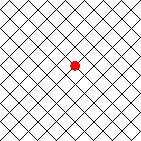
\includegraphics[scale=1.1]{figures/tikz/TFI/site_indices/site_index_a.pdf}
		}
	\end{minipage}	
	\par\medskip
	\begin{minipage}{1.0\textwidth}
		\hspace{20pt}
		\begin{tikzpicture}[scale=1, trim axis left, trim axis right]
			\begin{axis}[xlabel=$t$, ylabel=$\langle\hat{\sigma}_z\rangle$, grid=both, grid style={gray!20}, every axis plot/.append style={very thick}, scale only axis, height=\globalQuenchLargeFieldFigureHeight, width=\globalQuenchLargeFieldFigureWidth, xmin=-0.05, xmax=1.05, ymin=0.5, ymax=1.1]
				%	
				\addplot[color = 5blue1]
				table[x=t_tenpy, y=sz_chi_16, col sep=space]{figures/plots/TFI/global_quench/data/global_quench_g_6.0_tenpy_site_index_4_4_1.txt};
				%\addlegendentry{$\chi= 16$}
				%	
				\addplot[color = 5blue2]
				table[x=t_tenpy, y=sz_chi_32, col sep=space]{figures/plots/TFI/global_quench/data/global_quench_g_6.0_tenpy_site_index_4_4_1.txt};
				%\addlegendentry{$\chi= 32$}
				%	
				\addplot[color = 5blue3]
				table[x=t_tenpy, y=sz_chi_64, col sep=space]{figures/plots/TFI/global_quench/data/global_quench_g_6.0_tenpy_site_index_4_4_1.txt};
				%\addlegendentry{$\chi= 64$}
				%	
				\addplot[color = 5blue4]
				table[x=t_tenpy, y=sz_chi_128, col sep=space]{figures/plots/TFI/global_quench/data/global_quench_g_6.0_tenpy_site_index_4_4_1.txt};
				%\addlegendentry{$\chi= 128$}
				%	
				\addplot[color = 5blue5]
				table[x=t_tenpy, y=sz_chi_256, col sep=space]{figures/plots/TFI/global_quench/data/global_quench_g_6.0_tenpy_site_index_4_4_1.txt};
				%\addlegendentry{$\chi= 256$}
				%
			\end{axis}%
			\begin{axis}[scale only axis, height=\globalQuenchLargeFieldFigureHeight, width=\globalQuenchLargeFieldFigureWidth, every axis plot/.append style={very thick}, xmin=-0.05, xmax=1.05, ymin=0.5, ymax=1.1]
				%	
				\addplot[color = 3red1]
				table[x=t_disoTPS, y=sz_disoTPS_D_2, col sep=space]{figures/plots/TFI/global_quench/data/global_quench_g_6.0_disoTPS_site_index_4_4_1.txt};
				%\addlegendentry{$D = 2$}
				%	
				\addplot[color = 3red2]
				table[x=t_disoTPS, y=sz_disoTPS_D_4, col sep=space]{figures/plots/TFI/global_quench/data/global_quench_g_6.0_disoTPS_site_index_4_4_1.txt};
				%\addlegendentry{$D = 4$}
				%	
				\addplot[color = 3red3]
				table[x=t_disoTPS, y=sz_disoTPS_D_6, col sep=space]{figures/plots/TFI/global_quench/data/global_quench_g_6.0_disoTPS_site_index_4_4_1.txt};
				%\addlegendentry{$D = 5$}
				%
			\end{axis}%
		\end{tikzpicture}%
		\quad
		\raisebox{34.2pt}
		{%
			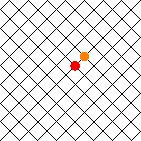
\includegraphics[scale=1.1]{figures/tikz/TFI/site_indices/site_index_b.pdf}
		}
	\end{minipage}
	\par\medskip
	\begin{minipage}{1.0\textwidth}
		\hspace{20pt}
		\begin{tikzpicture}[scale=1, trim axis left, trim axis right]
			\begin{axis}[xlabel=$t$, ylabel=$\langle\hat{\sigma}_z\rangle$, grid=both, grid style={gray!20}, every axis plot/.append style={very thick}, scale only axis, height=\globalQuenchLargeFieldFigureHeight, width=\globalQuenchLargeFieldFigureWidth, xmin=-0.05, xmax=1.05, ymin=0.9, ymax=1.05]
				%	
				\addplot[color = 5blue1]
				table[x=t_tenpy, y=sz_chi_16, col sep=space]{figures/plots/TFI/global_quench/data/global_quench_g_6.0_tenpy_site_index_5_5_0.txt};
				%\addlegendentry{$\chi= 16$}
				%	
				\addplot[color = 5blue2]
				table[x=t_tenpy, y=sz_chi_32, col sep=space]{figures/plots/TFI/global_quench/data/global_quench_g_6.0_tenpy_site_index_5_5_0.txt};
				%\addlegendentry{$\chi= 32$}
				%	
				\addplot[color = 5blue3]
				table[x=t_tenpy, y=sz_chi_64, col sep=space]{figures/plots/TFI/global_quench/data/global_quench_g_6.0_tenpy_site_index_5_5_0.txt};
				%\addlegendentry{$\chi= 64$}
				%	
				\addplot[color = 5blue4]
				table[x=t_tenpy, y=sz_chi_128, col sep=space]{figures/plots/TFI/global_quench/data/global_quench_g_6.0_tenpy_site_index_5_5_0.txt};
				%\addlegendentry{$\chi= 128$}
				%	
				\addplot[color = 5blue5]
				table[x=t_tenpy, y=sz_chi_256, col sep=space]{figures/plots/TFI/global_quench/data/global_quench_g_6.0_tenpy_site_index_5_5_0.txt};
				%\addlegendentry{$\chi= 256$}
				%
			\end{axis}%
			\begin{axis}[scale only axis, height=\globalQuenchLargeFieldFigureHeight, width=\globalQuenchLargeFieldFigureWidth, every axis plot/.append style={very thick}, xmin=-0.05, xmax=1.05, ymin=0.9, ymax=1.05]
				%	
				\addplot[color = 3red1]
				table[x=t_disoTPS, y=sz_disoTPS_D_2, col sep=space]{figures/plots/TFI/global_quench/data/global_quench_g_6.0_disoTPS_site_index_5_5_0.txt};
				%\addlegendentry{$D = 2$}
				%	
				\addplot[color = 3red2]
				table[x=t_disoTPS, y=sz_disoTPS_D_4, col sep=space]{figures/plots/TFI/global_quench/data/global_quench_g_6.0_disoTPS_site_index_5_5_0.txt};
				%\addlegendentry{$D = 4$}
				%	
				\addplot[color = 3red3]
				table[x=t_disoTPS, y=sz_disoTPS_D_6, col sep=space]{figures/plots/TFI/global_quench/data/global_quench_g_6.0_disoTPS_site_index_5_5_0.txt};
				%\addlegendentry{$D = 5$}
				%
			\end{axis}%
		\end{tikzpicture}%
		\quad
		\raisebox{34.2pt}
		{%
			\includegraphics[scale=1.1]{figures/tikz/TFI/site_indices/site_index_c.pdf}
		}
	\end{minipage}
	\caption{In this figure we show the time evolution of the $\langle\hat{\sigma}_z\rangle$ expectation value of a spin in the middle of the lattice and its neighbouring spins. The position of the spins is visualized in the lattice next to the plots. As a model we use the TFI model in the paramagnetic phase with a transverse field of $g = 6$, put on an $8\times8$ diagonal square lattice containing in total $N = 128$ spins. We compute the time evolution once with DMRG on a MPS and once with disoTPS with the parameters given in the text.}
	\label{fig:disoTPS_time_evolution_g_6}
\end{figure}
Finally, we want to test the time evolution in a less challenging regime, for which we used the TFI model at a transverse field of $g = 6$, which is well in the paramagnetic phase. In this regime, entanglement is expected to build up much slower than when simulating at the critical field. We again initialize an all-up-state $|\Psi\rangle = |\uparrow\rangle\otimes\cdots\otimes|\uparrow\rangle$ on the $8\times8$ square lattice but additionally flip a spin in the center. We then compute the time evolution of the $\langle\hat{\sigma}_z\rangle$ expectation value of the flipped center spin and neighbouring spins. The results are shown in figure \figref{fig:disoTPS_time_evolution_g_6}. Note that the DMRG reference simulation converges for much lower bond dimensions $\chi$ compared to figure \figref{fig:disoTPS_time_evolution_g_critical}. We also observe much better agreement of disoTPS TEBD and MPS DMRG.
	
	\appendix
	\addtocontents{toc}{\protect\setcounter{tocdepth}{0}}% This turns off sections
	
	\chapter{Optimization Problems for isometric Tensor Networks}
	\label{app:optimization_problems_for_isometric_tensor_networks}
	When discussing algorithms on isometric tensor networks, one often needs to find optimal tensors extremizing a given cost function $f$. In the most general case, $f$ is a function
\begin{equation}
	\label{eq:general_optimization_problem_of_isometric_tensor_networks_cost_function_multiple_input_tensors}
	f:\mathbb{C}^{m_1\times n_1}\times \dots \times \mathbb{C}^{m_K\times n_K} \to \mathbb{R},
\end{equation}
mapping $K$ tensors $T_1,\dots,T_K$ to a scalar cost value. Here, the tensors have already been reshaped into matrices, grouping together legs with incoming arrows and legs with outgoing arrows respectively. The tensors must satisfy certain constraints. If a tensor $T_i$ posesses both legs with incoming arrows and legs with outgoing arrows, it must satisfy the isometry constraint $T_i^\dagger T_i = \id$, where without loss of generalization we assumed $n_i \ge m_i$. If instead the tensor $T_j$ posesses only legs with incoming arrows (and thus is an orthogonality center), it is constrained to be normalized to one, $\lVert T_j\rVert_\text{F} = 1$. To summarize, we want to solve the optimization problem
\begin{equation}
	\label{eq:general_optimization_problem_of_isometric_tensor_networks_multiple_input_tensors}
	T_1^\text{opt}, \dots, T_K^\text{opt} = \underset{T_1,\dots T_K}{\text{argmax}}f\left(T_1, \dots T_K\right)
\end{equation}
under the constraints
\begin{equation}
	\label{eq:general_optimization_problem_of_isometric_tensor_networks_isometry_constraint}
	T_i^\dagger T_i = \id
\end{equation}
for isometries $T_i$ and
\begin{equation}
	\label{eq:general_optimization_problem_of_isometric_tensor_networks_ortho_center_constraint}
	\lVert T_j\rVert_\text{F} = 1
\end{equation}
for the orthogonality center $T_j$. \par
In the following, we will discuss several approaches for solving optimization problem \eqref{eq:general_optimization_problem_of_isometric_tensor_networks_multiple_input_tensors}. We will first assume that the input of the cost function is a single tensor $T$. If the cost function is linear, the problem is known as the \textit{orthogonal Procrustes problem} and we discuss its closed form solution in section \ref{sec:orthogonal_procrustes_problem}. Non-linear cost functions can be optimized by using the Evenbly-Vidal algorithm, see section \ref{sec:evenbly_vidal_algorithm}. Finally, we will discuss how cost functions of multiple tensors can be optimized in section \ref{sec:cost_functions_of_multiple_tensors}. \par
A different, more involved approach to solving the optimization problem is given by Riemannian optimization, which we discuss in appendix \ref{app:riemannian_optimization_of_isometries}.

\section{The orthogonal Procrustes problem}
\label{sec:orthogonal_procrustes_problem}
If the cost function is linear, it can be written as
\begin{equation}
	f(T) = \sum_{i=1}^{m}\sum_{j=1}^{n}\left[\alpha_{i,j}\Re\left(T_{i,j}\right) + \beta_{i,j} \Im\left(T_{i,j}\right)\right]
\end{equation}
with parameters $\alpha_{i,j}, \beta_{i,j} \in \mathbb{R}$. Introducing the \textit{environment tensor} $E\in\mathbb{C}^{m\times n}$ as $E_{i,j} = \alpha_i + \i \beta_j$ we can write the cost function as
\begin{equation}
	f(T) = \sum_{i=1}^{m}\sum_{j=1}^{n} \Re\left(E_{i,j}^*T_{i,j}\right) = \Re\Tr\left(E^\dagger T\right) = \Re\Tr\left(T^\dagger E\right).
\end{equation}
Maximizing $f(T)$ under the isometry constraint $T^\dagger T = \id$ is known as the orthogonal Procrustes problem and permits the closed form solution
\begin{equation}
	\label{eq:orthogonal_procrustes_problem_closed_form_solution}
	T^\text{opt} = \underset{T^\dagger T = \id}{\argmax} \Re\Tr\left(T^\dagger E\right) = UV^\dagger,
\end{equation}
where the matrices $U$ and $V$ are computed using an SVD $E = USV^\dagger$. To prove this result we insert the SVD into the cost function as
\begin{equation}
	\begin{split}
	f(T) &= \Re\Tr\left(ET^\dagger\right) = \Re\Tr\left(USV^\dagger T^\dagger\right) = \Re\Tr\left[\left(U\sqrt{S}\right)\left(\sqrt{S}V^\dagger T^\dagger\right)\right] \\
	&= \Re\left\langle\sqrt{S}U^\dagger,\sqrt{S}V^\dagger T^\dagger\right\rangle_\text{F}.
	\end{split}
\end{equation}
We next use the fact that the Frobenius inner product satisfies the Cauchy-Schwarz inequality to obtain the upper bound
\begin{equation}
	\begin{split}
		f(T) &= \Re\left\langle\sqrt{S}U^\dagger,\sqrt{S}V^\dagger T^\dagger\right\rangle_\text{F} \le \left\lVert\sqrt{S}U^\dagger\right\rVert_\text{F}\left\lVert\sqrt{S}V^\dagger T^\dagger\right\rVert_\text{F} \\
		&= \sqrt{\Tr\left(USU^\dagger\right)\Tr\left(TVSV^\dagger T^\dagger\right)} = \Tr\left(S\right),
	\end{split}
\end{equation}
where in the last step we used $U^\dagger U = \id$, $V^\dagger V = \id$, $T^\dagger T = \id$ and the cyclic property of the trace. This upper bound is reached by the solution
\begin{equation}
	F\left(T^\text{opt}\right) = \Re\Tr\left(USV^\dagger VU^\dagger\right) = \Tr\left(S\right),
\end{equation}
proving \eqref{eq:orthogonal_procrustes_problem_closed_form_solution}. \par
If the tensor $T$ must not satisfy the isometry condition but must be normalized to one, the closed form solution can be found as
\begin{equation}
	\label{eq:orthogonal_procrustes_problem_simple_case_closed_form_solution}
	T^\text{opt} = \underset{\left\lVert T\right\rVert = 1}{\argmax} \Re\Tr\left(T^\dagger E\right) = E/\left\lVert E\right\rVert.
\end{equation}
We arrive at this solution through a aimilar argument as before. First, we obtain an upper bound
\begin{equation}
	f(T) = \Re\Tr\left(T^\dagger E\right) = \Re\left\langle T, E\right\rangle_\text{F} \le \left\lVert T\right\rVert\left\lVert E\right\rVert = \left\lVert E\right\rVert
\end{equation}
using the Cauchy-Schwarz inequality and the normalization constraint $\left\lVert T\right\rVert = 1$. We proceed by showing that the upper bound is reached by $T^\text{opt}$,
\begin{equation}
	f(T^\text{opt}) = \Re\Tr\left(EE^\dagger/\left\lVert E\right\rVert\right) = \left\lVert E \right\rVert,
\end{equation}
proving \eqref{eq:orthogonal_procrustes_problem_simple_case_closed_form_solution}.

\section{The Evenbly-Vidal algorithm}
\label{sec:evenbly_vidal_algorithm}
In general the cost function $f(T)$ is not linear. For example, a non-linear cost function is encountered in the disentangling procedure when optimizing a MERA wave function \cite{}. It was proposed by Evenbly and Vidal \cite{} to linearize the cost function and to update the tensor $T$ iteratively using the closed form solutions from section \ref{sec:orthogonal_procrustes_problem}. Let us assume that the cost function $f(T)$ can be written as the contraction of a tensor network, where in general the tensor $T$ may appear multiple times. We contract all tensors except one of the tensors $T$ into an environment tensor $E_T \in\mathbb{C}^{n\times n}$ and the cost function becomes
\begin{equation}
	f(T)=\Re\Tr\left(E_TT\right).
\end{equation}
We now keep the environment $E_T$ fixed, trating it as if it were independant of $T$, and updating $T$ with the closed form solutions \eqref{eq:orthogonal_procrustes_problem_closed_form_solution} or \eqref{eq:orthogonal_procrustes_problem_simple_case_closed_form_solution}. This is repeated until $T$ is converged. If and how fast $T$ converges depends on the details of the cost fucntion, but connvergence cannot be guaranteed for arbitrary cost functions. This procedure is discussed in more detail and for general cost functions in appendix \ref{app:}\par
One can also use Riemannian optimization for the optimization of general non-linear cost functions of isometries. This method is more powerful but also more involved and is discussed in appendix \ref{app:riemannian_optimization_of_isometries}.

\section{Cost functions of multiple tensors}
\label{sec:cost_functions_of_multiple_tensors}
cost functions of multiple tensors $T_1, \dots T_K$ can be optimized iteratively via an algorithm similar to the Evenbly-Vidal algorithm. The idea is to optimize one tensor atr a time, keeping all other tensors fixed. To optimize the tensor $T_i$, we again contract all other tensors into an environment tensor $E$. If the environment tensor is independent of $T_i$ (i.e. if the cost function is linear in $T_i$), we can update the tensor with the closed form solutions of section \ref{sec:orthogonal_procrustes_problem}. Such an update is locally optimal in the sense that it maximizes $f(T_1, \dots, T_K)$ for fixed tensors $T_j$, $j\neq i$. If the environment tensor is dependant of $T_i$, we need to use the Evenbly-Vidal algorithm (see section \ref{sec:evenbly_vidal_algorithm}) or Riemannian optimization (see appendix \ref{app:riemannian_optimization_of_isometries}). If the cost function is linear in all tensors $T_1, \dots, T_K$ and bounded $f(T_1, \dots, T_K) \le c\in\mathbb{R}$, this algorithm is guaranteed to converge, since each local update is optimal and thus the cost function can never decrease. \par
An alternative approach for optimizing a cost function of multiple tensors is given by Riemannian optimization over product manifolds \cite{cite:riemannian_optimization_isometric_tensor_networks}, which we discuss briefly in appendix \ref{} \todo{Where do we discuss this?}
	
	\chapter{Riemannian Optimization of Isometries}
	\label{app:riemannian_optimization_of_isometries}
	In this appendix we provide a brief introduction to the problem of optimizing a cost function on the constrained set of isometric matrices. This problem can be solved by performing Riemannian Optimization on the matrix manifold of isometric matrices, which is called the Stiefel manifold. For a more in-depth introduction to the topic we recommend the excellent book \cite{cite:optimization_on_matrix_manifolds}. A discussion of Riemannian optimization of complex matrix manifolds in the context of quantum physics and isometric tensor networks can be found at \cite{cite:riemannian_geometry_automatic_differentiation_quantum_physics, cite:riemannian_optimization_isometric_tensor_networks}. An implementation of Riemannian Optimization on the real Stiefel manifold and other matrix manifolds in python is given in \cite{cite:pymanopt}. Some parts of this implementation were also used in our implementation.

\section{The complex Stiefel manifold}
\label{sec:the_complex_stiefel_manifold}
We define the \textit{complex Stiefel manifold} $\Stiefel$ with $n \ge p$ as the set of all isometric $n\times p$ matrices:
\begin{equation}
	\label{eq:Stiefel_manifold_definition}
	\Stiefel \coloneqq \left\{X\in\mathbb{C}^{n\times p}: X^\dagger X = \id\right\}.
\end{equation}
In particular, for $n = p$, the complex Stiefel manifold reduces to the set of unitary matrices $U(n)$. One can show, similar to \cite{cite:optimization_on_matrix_manifolds}, that the complex Stiefel manifold is naturally an embedded submanifold of the Euclidian vector space $\mathbb{C}^{n\times p} \cong \mathbb{R}^{2np}$ of general complex $n\times p$ matrices. \par
Tangent vectors on manifolds generalize the notion of directional derivatives. A mathematical definition of tangent vectors and tangent spaces of manifolds is given in \cite{cite:optimization_on_matrix_manifolds}. The set of all tangent vectors to a point $X\in\Stiefel$ is called the \textit{tangent space} $T_X \Stiefel$, which is given by \cite{cite:optimization_on_matrix_manifolds, cite:riemannian_optimization_isometric_tensor_networks}
\begin{equation}
	\label{eq:Stiefel_manifold_tangent_space}
	T_X \Stiefel = \left\{Z\in\mathbb{C}^{n\times p}:X^\dagger Z + Z^\dagger X = 0\right\}.
\end{equation}
An arbitrary element $\xi \in \mathbb{C}^{n\times p}$ from the embedding space $\mathbb{C}^{n\times p}$ can be projected to the tangent space $T_X \Stiefel$ by \cite{cite:optimization_on_matrix_manifolds, cite:riemannian_optimization_isometric_tensor_networks}
\begin{equation}
	\label{eq:Stiefel_manifold_project_to_tangent_space}
	P_X\xi = \xi - \frac{1}{2}X\left(X^\dagger\xi + \xi^\dagger X\right).
\end{equation}
Additionally, we will also need to define a notion of length that we can apply to tangent vectors. This can be done in the form of an \textit{inner product} on tangent spaces, called the \textit{Riemannian metric}. A natural metric for the tangent space $T_X \Stiefel$ of the Stiefel manifold is the Euclidean metric of the embedding space $\mathbb{C}^{n\times p}$, which is given by the real part of the Frobenius inner product:
\begin{equation}
	\label{eq:Stiefel_manifold_riemannian_metric}
	g_W: T_X \Stiefel \times T_X \Stiefel \to \mathbb{R}, \quad g_X(\xi_1, \xi_2) = \Re\Tr\left(\xi_1^\dagger\xi_2\right).
\end{equation}
Equipped with a Riemannian metric the Stiefel manifold becomes a Riemannian submanifold of $\mathbb{C}^{n\times p}$. \par
With these definition, we can now formulate the optimization problem as the problem of finding the isometry $W_\text{opt} \in \Stiefel$ that minimizes the cost function
\begin{equation}
	\label{eq:Optimization_cost_function_definition}
	f: \Stiefel \to \mathbb{R}, \quad X \mapsto f(X).
\end{equation}

\section{Gradients, retractions, and vector transport}
\label{sec:gradients_retractions_vector_transport}
First order optimization algorihms like Gradient Descent and Conjugate Gradients use the gradient of the cost function to update the search direction at each iteration. In the case of the Stiefel manifold and the cost function \eqref{eq:Optimization_cost_function_definition}, we first define the matrix of partial derivatives $D \in \mathbb{C}^{n\times p}$ of $f$ at $X\in\Stiefel$ by
\begin{equation}
	\label{eq:Optimization_partial_derivative}
	D_{ij} \coloneqq \left.\frac{\partial f}{\partial \Re\left(X_{ij}\right)}\right|_{X} + \iu \left.\frac{\partial f}{\partial \Im\left(X_{ij}\right)}\right|_{X}.
\end{equation}
With this definition, the directional derivative $\text{D}f(X)[Z]$ at $X\in\Stiefel$ in direction $Z\in\mathbb{C}^{n\times p}$ is simply given by an inner product of $D$ with the direction $Z$, using the Riemannian metric \eqref{eq:Stiefel_manifold_riemannian_metric}:
\begin{equation}
	\label{eq:riemannian_optimization_directional_derivative_partial_derivatives}
	\begin{split}
		g_X(D, Z) &= \Re\Tr\left(D^\dagger Z\right) = \Re\sum_{ij} D_{ij}^*Z_{ij} \\
		&= \sum_{ij} \left(\left.\frac{\partial f}{\partial \Re\left(X_{ij}\right)}\right|_{X}\Re Z_{ij} + \left.\frac{\partial f}{\partial \Im\left(X_{ij}\right)}\right|_{X} \Im Z_{ij}\right) \\
		&\eqqcolon \text{D}f(X)[Z].
	\end{split}
\end{equation}
With this we can now define the gradient $\nabla f(X)$ of $f$ at $X\in\Stiefel$ as the projection of the partial derivative matrix \eqref{eq:Optimization_partial_derivative} to the tangent space \cite{cite:optimization_on_matrix_manifolds, cite:riemannian_optimization_isometric_tensor_networks}:
\begin{equation}
	\label{eq:riemannian_optimization_gradient_of_cost_function}
	\nabla f(X) \coloneqq P_X D = D - \frac{1}{2}X\left(X^\dagger D + D^\dagger X\right),
\end{equation}
where we used the projection \eqref{eq:Stiefel_manifold_project_to_tangent_space}.

\section{Conjugate Gradients}
\label{sec:conjugate_gradients}
The \textit{Conjugate Gradients} (CG) algorithm \cite{cite:introduction_to_CG_without_pain, cite:a_survey_of_nonlinear_CG_methods, cite:algorithm_CG_DESCENT_a_CG_method_with_guaranteed_descent} was initially introduced as an iterative method for solving large systems of linear equations of the form $Ax = b$ with a known vector $b$, a known, square, positive-definite matrix $A$, and an unknown vector $x$. It is however found that the method also works well on non-linear problems, often outperforming simple Gradient Descent. We will only discuss non-linear GD, for a introduction to linear GD see \cite{cite:introduction_to_CG_without_pain}. The main idea of CG is to compute an accumulated search direction $\xi_{k}$ from the gradients at previous iterates as
\begin{equation}
	\xi_k = -\nabla f(X_{k}) + \beta_{k} \xi_{k-1}.
\end{equation}
There has been a lot of research on determining good algorithms for computing the parameter $\beta_{k}$. Two popular choices are the \textit{Fletcher-Reeves formula} \cite{cite:optimization_on_matrix_manifolds}
\begin{equation}
	\beta_{k}^\text{FR}\frac{\langle\nabla f(x_{k}), \nabla f(x_{k})\rangle}{\langle\nabla f(x_{k-1}), \nabla f(x_{k-1})\rangle}
\end{equation}
and the \textit{Polak-Ribiere formula} \cite{cite:optimization_on_matrix_manifolds}
\begin{equation}
	\beta_{k}^\text{PR}\frac{\langle\nabla f(x_{k}), \nabla f(x_{k})-\nabla f(x_{k-1})\rangle}{\langle\nabla f(x_{k-1}), \nabla f(x_{k-1})\rangle},
\end{equation}
where $\langle\cdot,\cdot\rangle$ denotes the inner product of the vector space. After the search direction is computed, the next iterate is computed as $x_{k+1} = x_k + \alpha_k \xi_k$, where $\alpha_k$ is determined using a suitable line-search procedure, e.g. Armijo line search \cite{cite:optimization_on_matrix_manifolds}. The initial search direction is simply the direction of steepest descent, $\xi_0 = -\nabla f(x_0)$. \par
On Riemannian manifolds, the inner product $\langle\cdot,\cdot\rangle$ is replaced by the Riemannian metric. Additionally, a retraction must be used for updating the iterates, $x_{k+1} = R_{\xi_k}(\alpha_k)$. Finally, a suitable vector transport $T_{k-1\rightarrow k}$ must be used for computing $\beta_k$, if the formula requires gradients or search direction from previous iterates. For an in-depth explanation of how CG on the Stiefel manifold can be implemented, see \cite{cite:optimization_on_matrix_manifolds, cite:a_riemannian_CG_method_for_optimization_on_the_Stifel_manifold, cite:riemannian_optimization_isometric_tensor_networks}. \par
In our implementation we additionally used Powell's restart strategy \cite{cite:on_the_use_of_powells_restart_strategy, cite:a_survey_of_nonlinear_CG_methods, cite:pymanopt}, which can significantly inprove the efficiency of CG.

\section{Trust Region Method}
\label{sec:trust_region_method}
\textit{Trust-region methods} (TRM) are a class of second order optimization techniques that are known for their desirable global convergence properties with a local superlinear rate of convergence \cite{cite:optimization_on_matrix_manifolds, cite:trust_region_methods_on_riemannian_manifolds}. The main idea of the TRM is to locally approximate the cost function $f$ by a quadratic model
\begin{equation}
	m_{X_k}(\nu) = f(X_k) + \langle \nabla f(X_k), \nu\rangle + \frac{1}{2}\langle \text{Hess}f(x_k)[\eta], \eta\rangle,
\end{equation}
in a \textit{trust-region} $\langle\eta,\eta\rangle \le \Delta_k^2$ of radius $\Delta_k$ around the current iterate $X_k$. To define this model, one must compute the Hessian vector-product $\text{Hess}f(X_k)[\eta]$ or an approximation thereof. On Riemannian submanifolds of Euclidean vector spaces, the Hessian can be computed by projecting the directional derivative $\text{D}(\nabla f(X_k))\left[\nu\right]$ of the gradient $\nabla f(X_k)$ from the embedding space to the tangent space of $X_k$ \cite{cite:optimization_on_matrix_manifolds}. Since the Stiefel manifold is such a Riemannian submanifold, it holds
\begin{equation}
	\label{eq:hessian_vector_product}
	\text{Hess}f(X_k)[\eta] = P_{X_k} \text{D}(\nabla f(X_k))\left[\nu\right]
\end{equation}
with the projection \eqref{eq:Stiefel_manifold_project_to_tangent_space}. Optimizing the cost function on the quadratic model inside the trust-region is called the \textit{trust-region subproblem} and can be solved via \textit{truncated CG}, which converges quickly on the quadratic model \cite{cite:optimization_on_matrix_manifolds}. The solution of the trust-region subproblem is a vector $\eta_\text{opt}$. The proposed next iterate is then given by moving in the direction $\eta_\text{opt}$ as $X_{k+1} = R_{\eta_\text{opt}}(1)$. To decide if the next iterate is accepted or not, we proceed to compute the quotient
\begin{equation}
	\rho_k \coloneqq \frac{f(X_k) - f(R_{\eta_\text{opt}}(1))}{m_{X_k}(0) - m_{X_k}(\eta_\text{opt})}.
\end{equation}
The quotient $\rho$ is a measure of how well the cost function is represented by the model $m_{X_k}$. If $\rho$ is to small, the model is very inaccurate. In this case the proposed update step must be rejected and the trust-region radius $\Delta_k$ must be reduced. If $\rho_k$ is close to one, the model is a good approximation of the cost function, and thus the update step can be accepted and the trust-region radius increased. If $\rho_k \gg 1$, the model is inaccurate, but the iteration still produces a significant decrease in the cost. One possible strategy in this situation is to accept the update and to increase the trust-region radius, hoping that this behaviour will remain in the following iterations, decreasing the cost further. This finally concludes one iteration of the TRM. For more details on the TRM on Riemannian manifolds, see \cite{cite:optimization_on_matrix_manifolds, cite:trust_region_methods_on_riemannian_manifolds, cite:pymanopt}.
	
	\chapter{Initialization of the Disentangling Unitary}
	
	\chapter{Computing the Gradient and Hessian of the Disentangling Cost Functions}
	\label{app:computation_of_gradient_and_hvp_for_riemannian_optimization}
	In this appendix we compute the Riemannian gradients and Hessian-vector products for the cost functions \eqref{eq:YB_move_disent_cost_function_truncation_error} and \eqref{eq:renyi_entropy}. For this it is first necessary to derive the derivative of the complex-valued singular value decomposition (SVD), which we show in Section \ref{sec:derivative_of_SVD}. The derivation is similar to \cite{cite:differentiating_the_svd}. We then proceed by deriving the gradients in section \ref{sec:renyi_trunc_gradients} and the hessian-vector products in section \ref{sec:renyi_trunc_hvps}.
\section{Derivative of the SVD}
\label{sec:derivative_of_SVD}
Let $A\in\mathbb{C}^{m\times n}$ of rank $k \le \min(m,n)$. The SVD of $A$ is defined as $A = USV^\dagger$, with $U\in\mathbb{C}^{m\times k}$, $S\in\mathbb{R}^{k\times k}$ diagonal, $V\in\mathbb{C}^{n\times k}$ and
\begin{equation}
	\label{eq:derivative_svd_eq_1}
	 U^\dagger U = V^\dagger V = \id_k.
\end{equation}
In this definition we already truncated singular values $s_j = 0$, such that $S$ has only non-zero entries on the diagonal. Let $\text{d}A\in\mathbb{C}^{m\times n}$ be an infinitesimal change of $A$. We are interested in the infinitesimal changes $\text{d}U$, $\text{d}S$ and $\text{d}V$ that are obtained when performing the SVD $(A+\text{dA}) = (U + \text{d}U)(S + \text{d}S)(V + \text{d}V)^\dagger$. Up to first order we obtain
\begin{equation}
	\label{eq:derivative_svd_eq_2}
	\text{d}A = \text{d}USV^\dagger + U\text{d}SV^\dagger + US\text{d}V^\dagger.
\end{equation}
Differentiating Equation \eqref{eq:derivative_svd_eq_1} yields $\text{d}U^\dagger U + U^\dagger\text{d}U = 0$ and $\text{d}V^\dagger V + V^\dagger\text{d}V = 0$. It follows that $\text{d}\Omega_U \coloneqq U^\dagger\text{d}U$ and $\text{d}\Omega_V \coloneqq V^\dagger\text{d}V$ are $k\times k$ anti-hermitian matrices. \par
One can always find matrices $U_\perp\in\mathbb{C}^{m\times(m-k)}$ and $V_\perp\in\mathbb{C}^{n\times(n-k)}$ such that $\left[U\,U_\perp\right]$ and $\left[V V_\perp\right]$ are unitary and it holds $U^\dagger U_\perp = 0$ and $V^\dagger V_\perp = 0$. This procedure is called unitary completion and can for example be computed by using the Gram-Schmidt algorithm. The notation $\left[U\,U_\perp\right]$ means stacking the columns of $U$ and $U_\perp$ to form a $m\times m$ matrix. We may now expand $\text{d}U$ as
\begin{equation}
	\label{eq:dOmega_U_definition}
	\text{d}U = U\text{d}\Omega_U + U_\perp\text{d}K_U
\end{equation}
and $\text{d}V$ as
\begin{equation}
	\label{eq:dOmega_V_definition}
	\text{d}V = V\text{d}\Omega_V + V_\perp\text{d}K_V,
\end{equation}
with $\text{d}K_U\in\mathbb{C}^{(m-k)\times k}$ and $\text{d}K_V\in\mathbb{C}^{(n-k)\times k}$ yet to be determined. We proceed by left-multiplying \eqref{eq:derivative_svd_eq_2} by $U^\dagger$ and right-multiplying by $V$ to obtain
\begin{equation}
	\label{eq:svd_derivative_P_definition}
	\begin{split}
		\text{d}P \coloneqq U^\dagger\text{d}AV &= U^\dagger\text{d}US + \text{d}S + S\text{d}V^\dagger V \\
		&= \text{d}\Omega_U S + \text{d}S + S\text{d}\Omega_V^\dagger.
	\end{split}
\end{equation}
Since $\text{d}\Omega_U$ and $\text{d}\Omega_V$ are anti-hermitian, there diagonal elements are purely imaginary. However, $\text{d}S$ is a diagonal matrix with purely real entries. Thus it is immediately clear that
\begin{equation}
	\label{eq:dS_final}
	\text{d}S = \id_k \circ \Re\left[\text{d}P\right],
\end{equation}
with the \textit{Hadamard product} $(A\circ B)_{i,j} = A_{i,j}\cdot B_{i,j}$. It further follows
\begin{equation}
	\label{eq:derivative_svd_eq_3}
	\text{d}\Omega_US - S\text{d}\Omega_V = \id_k\circ i\Im\left[\text{d}P\right] + \bar{\id}_k\circ\text{d}P.
\end{equation}
Here, the notation $\bar{\id}_k$ means a $k\times k$ matrix with zeros on the diagonal and ones everywhere else. Taking the complex conjugate of \eqref{eq:derivative_svd_eq_3} yields \begin{equation}
	\label{eq:derivative_svd_eq_4}
	-S\text{d}\Omega_U + \text{d}\Omega_V S = -\id_k\circ i\Im\left[\text{d}P\right] + \bar{\id}_k\circ\text{d}P^\dagger.
\end{equation}
To proceed we right-multiply \eqref{eq:derivative_svd_eq_3} by $S$, left-multiply \eqref{eq:derivative_svd_eq_4} by $S$ and add the two equations together, yielding
\begin{equation}
	\label{eq:equation_for_solving_dOmega_U}
	\text{d}\Omega_U S^2 - S^2 \text{d}\Omega_U = \bar{\id}_k\circ S\text{d}P + \bar{\id}_k\circ \text{d}P^\dagger S = \bar{\id}_k\circ\left[\text{d}PS+S\text{d}P^\dagger\right],
\end{equation}
where we used the fact that $D(A\circ B) = DA\circ B = A\circ DB$ and $(A\circ B)D = AD\circ B = A\circ BD$ for diagonal matrices $D$. We now want to solve Equation \eqref{eq:equation_for_solving_dOmega_U} for $\text{d}\Omega_U$. The solution is given by
\begin{equation}
	\label{eq:derivative_svd_eq_5}
	\text{d}\Omega_U = F\circ\left[\text{d}PS+S\text{d}P^\dagger\right]
\end{equation}
with 
\begin{equation}
	\label{eq:svd_derivative_F_definition}
	F_{i,j} \coloneqq \begin{cases}
		\frac{1}{d_j^2-d_i^2} &i \neq j\\
		0 &i = j
	\end{cases},
\end{equation}
which can be easily checked by inserting. We can obtain a similar equation for $\text{d}\Omega_V$ by left-multiplying \eqref{eq:derivative_svd_eq_3} by $S$ and right-multiplying \eqref{eq:derivative_svd_eq_4} by $S$ before adding the two equations. The resulting equation is solved by
\begin{equation}
	\label{eq:derivative_svd_eq_6}
	\text{d}\Omega_V = F\circ\left[S\text{d}P+\text{d}P^\dagger S\right].
\end{equation}
Equations \eqref{eq:derivative_svd_eq_5} and \eqref{eq:derivative_svd_eq_6} do not fix the diagonals of $\text{d}\Omega_U$ and $\text{d}\Omega_V$. We can determine these remaining free parameters by looking at the diagonal elements of equation \eqref{eq:derivative_svd_eq_3}:
\begin{equation}
	\begin{split}
		&\id_k\circ\left[\text{d}\Omega_US-S\text{d}\Omega_V\right] = \id\circ i\Im\left[\text{d}P\right] \\
		\Rightarrow \quad &\id_k\circ\left[\text{d}\Omega_U-\text{d}\Omega_V\right] = \id_k\circ i\Im\left[\text{d}P\right]S^{-1}.
	\end{split}
\end{equation}
We can solve this equation by setting
\begin{equation}
	\begin{split}
		\text{d}\Omega_U &= F\circ\left[\text{d}PS + S\text{d}P^\dagger\right] + \id_k\circ\text{d}D,\\
		\text{d}\Omega_V &= F\circ\left[S\text{d}P + \text{d}P^\dagger S\right] - \id_k\circ\text{d}D,
	\end{split}
\end{equation}
with
\begin{equation}
	\text{d}D \coloneqq \frac{i}{2}\Im\left[\text{d}P\right]S^{-1}.
\end{equation}
It remains to find $\text{d}K_U$ and $\text{d}K_V$. We can compute $\text{d}K_U$ by left-multiplying \eqref{eq:derivative_svd_eq_2} by $U_\perp^\dagger$ and right-multiplying by $VS^{-1}$, yielding
\begin{equation}
	\label{eq:derivative_svd_eq_7}
	\text{d}K_U = U_\perp^\dagger \text{d}AVS^{-1}.
\end{equation}
Similarly, we can left-multiply \eqref{eq:derivative_svd_eq_2}$^\dagger$ by $V_\perp^\dagger$ and right-multiplying by $US^{-1}$ to obtain
\begin{equation}
	\label{eq:derivative_svd_eq_8}
	\text{d}K_V = V_\perp^\dagger\text{d}A^\dagger US^{-1}.
\end{equation}
Putting everything together, we obtain
\begin{equation}
	\label{eq:final_solution_svd_derivative}
	\begin{split}
		\text{d}U &= U\left(F\circ\left[\text{d}PS+S\text{d}P^\dagger\right] + \id_k\circ\text{d}D\right) + \left(\id_m-UU^\dagger\right)\text{d}AVS^{-1}. \\
		\text{dS} &= \id_k\circ\Re\left[\text{d}P\right]. \\
		\text{d}V &= V\left(F\circ\left[S\text{d}P+\text{d}P^\dagger S\right] - \id_k\circ\text{d}D\right) + \left(\id_n-VV^\dagger\right)\text{d}AUS^{-1},
	\end{split}
\end{equation}
with $\text{d}P$ defined in Equation \eqref{eq:svd_derivative_P_definition} and $F$ defined in Equation \eqref{eq:svd_derivative_F_definition}. To arrive at the final expressions for $\text{d}U$ and $\text{dV}$ we used the fact that $M_U \coloneqq \left[U\,U_\perp\right]$ and $M_V \coloneqq \left[V V_\perp\right]$ are unitary and thus $M_UM_U^\dagger = UU^\dagger + U_\perp U_\perp^\dagger = \id_m$ and similarly $VV^\dagger + V_\perp V_\perp^\dagger = \id_n$ to eliminate $U_\perp U_\perp^\dagger$ and $V_\perp V_\perp^\dagger$. \par
There is one small subtlety left to discuss. The SVD is not unique, but has a gauge degree of freedom: A diagonal matrix of complex phases $\Lambda_{j,j} = e^{i\theta_j}$ can be inserted as $A = USV^\dagger = U^\prime S V^{\prime\dagger} = (U\Lambda)S(V\Lambda)^\dagger$. This means that the exact values of $\text{d}U$ and $\text{d}V$ are ill-defined and it is only possible to compute derivatives of functions that are gauge-invariant, i.e. functions where $\Lambda$ is cancelled with its adjoint.
%
%
\section{Gradients}
%
%
\label{sec:renyi_trunc_gradients}
We now compute Riemannian gradients for the two cost functions discussed in Section \ref{sec:YB_move_svd_disentangle}, namely the truncation error
\begin{equation}
	\label{eq:appendix_trunc_error_cost_function}
	f_\text{trunc}\left(U,\theta\right) = \sqrt{\sum_{\mu = \chi+1}^{\chi D^2}S_\mu^2} = \sqrt{1 - \sum_{\mu = 1}^{\chi}S_\mu^2}
\end{equation}
and the Rényi-entropy
\begin{equation}
	\label{eq:appendix_renyi_cost_function}
	f_\text{Rényi}\left(U,\theta,\alpha\right) = \frac{1}{1-\alpha}\log\Tr\left(\rho^\alpha\right) = \frac{1}{1-\alpha}\log\left(\sum_{\mu=1}^{\chi D^2}S_\mu^{2\alpha}\right).
\end{equation}
The singular values stem from the SVD $U\theta$ = $XSY$ as shown in figure \figref{fig:disentangling_theta_definition}. We first compute the derivative of a single singular value $S_\mu$ with respect to $U$. Using the product rule for matrices \cite{cite:the_matrix_cook_book} and the derivative of the SVD \eqref{eq:final_solution_svd_derivative}, we obtain
\begin{center}
	\includegraphics[scale=1]{figures/tikz/gradient_and_hvp/derivative_of_s_mu/derivative_of_s_mu.pdf}
\end{center}
We can then use this result to compute the derivative of the truncation error as
\begin{equation}
	\frac{\text{d}}{\text{d}U}f_\text{trunc}(U,\theta) = -\frac{1}{f_\text{trunc}(U,\theta)}\sum_\mu S_\mu \frac{\text{d}S_\mu}{\text{d}U}
\end{equation}
and the derivative of the Rényi-entropy as
\begin{equation}
	\frac{\text{d}}{\text{d}U}f_\text{Rényi}(U,\theta,\alpha) = \frac{2\alpha}{1-\alpha}\frac{1}{\sum_\mu S_\mu^{2\alpha}} \sum_\mu S_\mu^{2\alpha-1}\frac{\text{d}S_\mu}{\text{d}U}.
\end{equation}
As a last step, the derivatives must be projected back to the tangent space of $U$, see Equation \eqref{eq:riemannian_optimization_gradient_of_cost_function}. We obtain
\begin{equation}
	\left(\nabla f_\text{trunc}\left(U,\theta\right)\right)_{i,j,k,l} = \frac{1}{2f_\text{trunc}\left(U,\theta\right)}\xi^\text{trunc}_{i,j,k,l}
\end{equation}
and
\begin{equation}
	\left(\nabla f_\text{Rényi}\left(U,\theta,\alpha\right)\right)_{i,j,k,l} = \frac{\alpha}{1-\alpha}\frac{1}{\sum_\mu S_\mu^{2\alpha}}\xi^\text{Rényi}_{i,j,k,l}
\end{equation}
respectively, with
\begin{center}
	\includegraphics[scale=1]{figures/tikz/gradient_and_hvp/xi_definition/xi_definition.pdf}
\end{center}
where $\tilde{S} = S$ for $\xi^\text{trunc}$ and $\tilde{S} = S^{2\alpha-1}$ for $\xi^\text{Rényi}$.
%
%
\section{Hessian-Vector Products}
\label{sec:renyi_trunc_hvps}
%
%
In this section we compute the Hessian-vector product of $\nabla f$ and $\Delta U$. We start by first calculating the directional derivative of the gradient in direction $\Delta U$
\begin{equation}
	\text{D}\left(\nabla f\right)\left[\Delta U\right],
\end{equation}
which we subsequently need to project to the tangent space of $U$. For matrix multiplication it holds\cite{cite:the_matrix_cook_book}
\begin{equation}
	\text{D}\left(AB\right)\left[\Delta A\right] = \Delta AB.
\end{equation}
Directional derivatives of $X$, $U$ and $Y$ can be obtained with equation \eqref{eq:final_solution_svd_derivative} by setting $\text{d}A = \Delta U\theta$. The final result are the directional derivatives
\begin{multline}
	\big((\text{D}(\nabla f_\text{trunc})[\Delta U]\big)_{i,j,k,l} = \\
	-\frac{1}{2f_\text{trunc}(U, \theta)} \cdot \left\{\frac{1}{f_\text{trunc}(U,\theta)^2}\sum_{\mu=1}^{\chi}S_\mu\big(\text{D}S_\mu[\Delta U]\big)\xi_{i,j,k,l} + G^\text{trunc}_{i,j,k,l}\right\}
\end{multline}
and
\begin{multline}	
	\big(\text{D}(\nabla f_\text{Rényi})[\Delta U]\big)_{i,j,k,l} = \\
	\frac{\alpha}{1-\alpha} \left\{\frac{2\alpha}{\left(\sum_\mu S_\mu^{2\alpha}\right)^2}\sum_\mu S_\mu^{2\alpha-1}\text{d}S_\mu\xi_{i,j,k,l} + \frac{1}{\sum_\mu S_\mu^{2\alpha}}G^\text{Renyi}_{i,j,k,l}\right\}
\end{multline}
with the definition of $G^\text{trunc}$ and $G^\text{Rényi}$ given in tensor diagram notation in Figure \figref{fig:G_definition}. Finally, The derivatives must be projected to the tangent space of $U$, see Equation \eqref{eq:riemannian_optimization_gradient_of_cost_function}.
\begin{figure}
	\centering
	\includegraphics[scale=0.9]{figures/tikz/gradient_and_hvp/G_definition/G_definition.pdf}
	\caption{In this figure we give the definition for $G^\text{trunc}$ and $G^\text{Rényi}$ in tensor diagram notation. For $G^\text{trunc}$ we set  $\tilde{S} = S$ and for $G^\text{Rényi}$ we set  $\tilde{S} = S^{2\alpha-1}$. The definition of $\text{d}(X\tilde{S}Y)$ is given in figure \protect\figref{fig:dXSY_definition}}
	\label{fig:G_definition}
\end{figure}
\begin{figure}
	\centering
	\subcaptionbox{\label{fig:dXSY_definition_trunc}}
	{%
		\includegraphics[scale=1]{figures/tikz/gradient_and_hvp/dXSY_definition/dXSY_definition_a.pdf}
	}
	\par\bigskip
	\subcaptionbox{\label{fig:dXSY_definition_rewnyi}}
	{%
		\includegraphics[scale=1]{figures/tikz/gradient_and_hvp/dXSY_definition/dXSY_definition_b.pdf}
	}
	\caption{The definitions for (a) $\text{d}(XSY^\dagger)$ and (b) $\text{d}(XS^{2\alpha-1}Y^\dagger)$ are given in tensor diagram notation. In (b), we use $S_\mu^\prime \coloneqq (2\alpha-1)S_\mu^{2\alpha-2}\text{d}S_\mu$.}
	\label{fig:dXSY_definition}
\end{figure}
	
	
	\backmatter
	\printbibliography
	
\end{document}